% =====================================================================
%  KELP — Numerical Methods and Implementation: A Reference Manual
%
%  Build:   make            (pins the TeX Live 2025 path; runs latexmk)
%           make -C manual
%  Single chapter while drafting: uncomment \includeonly below.
% =====================================================================
\documentclass[11pt,oneside]{book}
% =====================================================================
%  preamble.tex — shared packages, page geometry, code listings,
%  bibliography and cross-referencing for the KELP manual.
%  pdfLaTeX toolchain (TeX Live 2025).
% =====================================================================

% --- fonts / encoding ---
\usepackage[T1]{fontenc}
\usepackage[utf8]{inputenc}
\usepackage{lmodern}
\usepackage{microtype}
\usepackage{textcomp}

% --- page geometry ---
\usepackage[a4paper,margin=2.6cm,headheight=14pt]{geometry}

% --- mathematics ---
\usepackage{amsmath}
\usepackage{amssymb}
\usepackage{mathtools}
\usepackage{bm}
\usepackage{siunitx}
\sisetup{detect-all=true}

% --- tables / figures ---
\usepackage{graphicx}
\graphicspath{{figs/}}
\usepackage{booktabs}
\usepackage{array}
\usepackage{tabularx}
\usepackage{longtable}
\usepackage{multirow}
\usepackage{enumitem}
\usepackage{caption}
\captionsetup{font=small,labelfont=bf}

% --- colour ---
\usepackage{xcolor}
\definecolor{codebg}{rgb}{0.965,0.965,0.965}
\definecolor{codekw}{rgb}{0.13,0.29,0.53}
\definecolor{codecomment}{rgb}{0.30,0.50,0.30}
\definecolor{codestr}{rgb}{0.64,0.08,0.08}
\definecolor{lagblue}{rgb}{0.10,0.30,0.55}
\definecolor{lagnode}{rgb}{0.10,0.30,0.55}
\definecolor{lagelem}{rgb}{0.70,0.35,0.05}
\definecolor{kelp}{rgb}{0.78,0.10,0.10}
\definecolor{laggreen}{rgb}{0.15,0.45,0.25}

% --- diagrams ---
\usepackage{tikz}
\usetikzlibrary{calc,positioning,arrows.meta,decorations.pathmorphing,%
  decorations.markings,shapes.geometric,backgrounds,fit,patterns,angles,quotes}
\usepackage{pgfplots}
\pgfplotsset{compat=1.17}
% =====================================================================
%  style/tikz-styles.tex — reusable TikZ styles for the schematics.
%  Convention used throughout the schematics:
%    * mesh NODE          -> filled blue circle
%    * element CENTRE     -> filled orange square
%    * vertical INTERFACE -> grey horizontal rule / open marker
%    * the DRIFTER        -> red five-pointed star
% =====================================================================
\tikzset{
  meshnode/.style     ={circle,fill=lagnode,draw=lagnode,inner sep=0pt,minimum size=4pt},
  meshnodeopen/.style ={circle,draw=lagnode,fill=white,line width=0.7pt,inner sep=0pt,minimum size=4.5pt},
  elemcentre/.style   ={rectangle,fill=lagelem,draw=lagelem,inner sep=0pt,minimum size=4pt},
  interfacept/.style  ={circle,draw=gray!70,fill=white,inner sep=0pt,minimum size=3.5pt},
  drifter/.style      ={star,star points=5,star point ratio=2.3,fill=kelp,draw=kelp!60!black,inner sep=0pt,minimum size=8pt},
  meshedge/.style     ={draw=gray!65,line width=0.7pt},
  meshface/.style     ={draw=gray!65,line width=0.7pt,fill=lagblue!5},
  hilface/.style      ={draw=lagblue,line width=1.0pt,fill=lagblue!12},
  weightlbl/.style    ={font=\small\itshape,text=black},
  nodelbl/.style      ={font=\footnotesize,text=lagnode!75!black},
  elemlbl/.style      ={font=\footnotesize,text=lagelem!70!black},
  interface/.style    ={draw=gray!55,line width=0.6pt},
  velarrow/.style     ={-{Stealth[length=4pt]},line width=0.8pt,draw=lagblue},
  % pipeline / flowchart
  flowbox/.style      ={rectangle,rounded corners=2pt,draw=lagblue,fill=lagblue!8,
                        align=center,inner sep=4pt,minimum height=8mm,text width=44mm,font=\small},
  sidebox/.style      ={rectangle,rounded corners=2pt,draw=lagelem,fill=lagelem!8,
                        align=left,inner sep=5pt,text width=50mm,font=\footnotesize},
  flowarrow/.style    ={-{Stealth[length=5pt]},line width=1pt,draw=lagblue},
  looparrow/.style    ={-{Stealth[length=5pt]},line width=1pt,draw=lagblue!55,dashed},
  % particle-status state machine
  statebox/.style     ={rectangle,rounded corners=3pt,draw=black,align=center,
                        inner sep=4pt,minimum width=24mm,minimum height=8mm,font=\small},
  trans/.style        ={-{Stealth[length=5pt]},line width=0.9pt},
}


% --- code listings (dependency-free: no shell-escape / Pygments) ---
\usepackage{listings}
\lstdefinestyle{py}{%
  language=Python,
  basicstyle=\ttfamily\small,
  backgroundcolor=\color{codebg},
  keywordstyle=\color{codekw}\bfseries,
  commentstyle=\color{codecomment}\itshape,
  stringstyle=\color{codestr},
  numbers=left,numberstyle=\tiny\color{gray!70},
  breaklines=true,showstringspaces=false,
  frame=single,rulecolor=\color{gray!40},columns=fullflexible,
  aboveskip=1.0em,belowskip=0.6em,
}
\lstdefinelanguage{yaml}{%
  keywords={true,false,null},
  keywordstyle=\color{codekw},
  comment=[l]{\#},commentstyle=\color{codecomment}\itshape,
  morestring=[b]",morestring=[b]',stringstyle=\color{codestr},
  basicstyle=\ttfamily\small,showstringspaces=false,
}
\lstdefinestyle{cfg}{%
  language=yaml,backgroundcolor=\color{codebg},frame=single,
  rulecolor=\color{gray!40},basicstyle=\ttfamily\small,breaklines=true,
  aboveskip=1.0em,belowskip=0.6em,
}
\lstset{style=py}

% --- bibliography (author-year) ---
\usepackage[round,authoryear]{natbib}

% --- hyperlinks (load late) then cleveref ---
\usepackage[colorlinks=true,linkcolor=lagblue,citecolor=laggreen,%
  urlcolor=lagblue,breaklinks=true]{hyperref}
\usepackage[capitalise,noabbrev]{cleveref}

% --- index ---
\usepackage{makeidx}

% running heads
\usepackage{fancyhdr}
\pagestyle{fancy}
\fancyhf{}
\fancyhead[L]{\small\leftmark}
\fancyhead[R]{\small\thepage}
\renewcommand{\headrulewidth}{0.4pt}

% =====================================================================
%  notation.tex — shared mathematical and code-reference macros.
%  Symbol conventions (see also the front matter and Appendix B):
%    position  x = (lambda, phi, z)   longitude, latitude, depth (down +)
%    velocity  u = (u, v, W)           W = vertical velocity (down +)
%    w_i                                barycentric / interpolation weight
%    alpha                              interpolation fraction (time or depth)
%    s_fb = +-1                         integration direction (time_dir)
% =====================================================================

% ---- calculus ----
\newcommand{\dd}{\mathrm{d}}
\newcommand{\dt}{\Delta t}
\newcommand{\pd}[2]{\frac{\partial #1}{\partial #2}}

% ---- position & velocity ----
\newcommand{\pos}{\mathbf{x}}
\newcommand{\velvec}{\mathbf{u}}
\newcommand{\lonx}{\lambda}
\newcommand{\latx}{\phi}
\newcommand{\depx}{z}
\newcommand{\Wvel}{W}
\newcommand{\tdir}{s_{\mathrm{fb}}}

% ---- spherical metric (metres per degree) ----
\newcommand{\Mlat}{M_{\latx}}            % metres per degree latitude (111120)
\newcommand{\zzero}{z_{0}}               % metres per degree longitude = cos(phi) Mlat

% ---- interpolation ----
\newcommand{\bwt}[1]{w_{#1}}             % barycentric weight i
\newcommand{\interpfrac}{\alpha}

% ---- code references (typeset, not hyperlinked) ----
\newcommand{\code}[1]{\texttt{\small #1}}      % inline code token
\newcommand{\conf}[1]{\texttt{\small #1}}       % YAML config key
\newcommand{\fn}[1]{\texttt{\small #1}}         % function / symbol name
\newcommand{\srcfile}[1]{\texttt{\small #1}}    % source file path

% A left-bar "Source." callout that ties prose to the implementation.
\newcommand{\codeanchor}[1]{%
  \par\smallskip\noindent
  {\color{lagblue}\rule[-0.15em]{2.5pt}{1.05em}}\hspace{0.6em}%
  \begin{minipage}[t]{0.93\linewidth}\small\textbf{Source.}\enspace #1\end{minipage}%
  \par\smallskip}

% A "Code vs. documentation" note, marking where the engine's documentation
% diverges from the source. The manual follows the source.
\newcommand{\codenote}[1]{%
  \par\smallskip\noindent
  {\color{lagelem}\rule[-0.15em]{2.5pt}{1.05em}}\hspace{0.6em}%
  \begin{minipage}[t]{0.93\linewidth}\small\textit{Code vs.\ documentation.}\enspace #1\end{minipage}%
  \par\smallskip}

\makeindex

% \includeonly{chapters/02-architecture}   % fast single-chapter rebuilds

\begin{document}
\frontmatter
\begin{titlepage}
\centering
\vspace*{3cm}
{\Huge\bfseries \textsf{KELP}\par}
\vspace{0.6cm}
{\LARGE Numerical Methods and Implementation\par}
\vspace{0.3cm}
{\large A Reference Manual\par}
\vspace{1.4cm}
{\large Lagrangian particle tracking on the unstructured meshes\\[2pt]
of the FESOM family (FESOM2 and FESOM-C)\par}
\vfill
{\large\itshape Engine reference --- numerics and source linkage\par}
\vspace{0.4cm}
\vfill
\end{titlepage}

\chapter*{Abstract}
\addcontentsline{toc}{chapter}{Abstract}

We document \textsf{KELP}, a Lagrangian particle-tracking engine that
integrates the trajectories of passive particles through the velocity fields of
unstructured-mesh ocean circulation models, with primary support for the FESOM
family --- FESOM2, on purely triangular meshes, and FESOM-C, on mixed
triangular--quadrilateral meshes --- and with readers for ocean fields remapped to the HEALPix grid and
for structured NEMO grids.
This manual is a numerical and implementation reference: for each component of
the engine we state the governing equations, give the discrete formulae exactly
as implemented, illustrate the underlying geometry with schematics, and cite the
location of the corresponding Python source. We treat the engine as the object of
study rather than any particular application; the FESOM2 \emph{core2} global mesh recurs only as a
concrete example.

The material is organized along the path a single time step travels through the
solver: locating a particle on the unstructured mesh, with a proof that the nearest node found is the
nearest; interpolating the velocity in space (horizontally by barycentric or least-squares schemes,
vertically between depth interfaces or along sigma surfaces) and in time (by linear or monotone
piecewise-cubic reconstruction); advancing the position with an explicit or adaptive Runge--Kutta
scheme; and applying boundary conditions. Stochastic diffusion, the particle lifecycle, the
forcing reader, trajectory output, the configuration surface, verification, and
computational cost --- measured across thread layouts, mesh sizes, particle counts and node counts ---
are each treated in turn, and a final part describes the agent skills through which experiments are set
up, run and analysed. We point to the engine's
physics-validation tests --- the analytic-flow benchmarks, the vertical streamfunction
(continuity) conservation tests, the reversibility round-trip, and the checks against real model
output --- by name, as evidence that the
numerics behave as specified, without reproducing their internals.

\tableofcontents
\listoffigures
\chapter*{How to use this manual}
\addcontentsline{toc}{chapter}{How to use this manual}

This manual is designed for selective, non-linear reading: a reader with a
specific question should be able to turn directly to the relevant chapter without
reading the preceding material. To that end we adopt a consistent internal
structure and several navigation aids.

\paragraph{Chapter structure.} Each chapter opens with a short statement of what
the component does and where it sits in the per-step pipeline
(\cref{ch:arch}). It then develops the governing equations and the discrete
formulae as implemented, accompanied by a schematic that shows which mesh
entities (nodes, element centres, vertical interfaces) supply values and how they
are combined. Each substantive claim about the implementation is followed by a
\textbf{Source} callout naming the file and the function or line range that
realizes it, so that the manual and the code can be read side by side.

\paragraph{Finding a topic.} Three routes are provided. The table of contents
lists every section. \Cref{app:codemap} is a source-code map: it lists, per
subsystem, the authoritative source symbols and the manual section that explains
them, so a reader starting from the code can find the corresponding text. The
index collects symbols, configuration keys, and function names.

\paragraph{Conventions and symbols.} The sign and unit conventions used
throughout (positive-downward depth, the integration-direction factor, the
spherical metric, the distinction between fields stored at nodes, at element
centres, and at vertical interfaces) are stated once in the front matter section
that follows, and the complete symbol list is given in \cref{app:notation}.

\paragraph{Worked configuration.} Where a concrete size clarifies a choice, we refer to the FESOM2
\emph{core2} global mesh; the ready configurations shipped with the engine cover two-dimensional global runs,
a three-dimensional regional run, a structured-grid run and HEALPix runs. The examples illustrate the engine;
they are not the subject of this document.

\paragraph{Setting up a run.} A reader who wants to run an experiment rather than study the numerics can start
from \cref{ch:skills}, which describes how a described experiment becomes seeds, a configuration and a run
command, and how the output is turned into statistics and figures; \cref{app:config} lists every configuration
key.

\chapter*{Notation and conventions}
\addcontentsline{toc}{chapter}{Notation and conventions}

We collect here the conventions that recur throughout the manual. The complete
symbol list is given in \cref{app:notation}.

\paragraph{Position and velocity.} A particle position is the triple
$\pos=(\lonx,\latx,\depx)$ of longitude, latitude (both in degrees), and depth.
The model velocity is $\velvec=(u,v,\Wvel)$, with horizontal components $u,v$ in
metres per second and vertical component $\Wvel$ in metres per second.

\paragraph{Depth and vertical velocity are positive downward.} Depth $\depx$
increases from $0$ at the surface to the sea floor, and the vertical velocity
$\Wvel$ is positive for downwelling. Consequently the vertical position update
$\depx \mathrel{+}= \Wvel\,\dt$ deepens a particle in downwelling, so that sinking
is followed with the correct sign.

\paragraph{Integration direction.} The factor $\tdir\in\{+1,-1\}$ (the
configuration key \conf{time\_dir}) selects forward ($+1$) or backward ($-1$)
integration. The time step $\dt$ is always a positive quantity; the direction
enters by multiplying the interpolated velocity, so that backward integration is
a sign reversal of the sampled velocity rather than a separate code path
(\cref{ch:arch,ch:integration}).

\paragraph{The spherical metric.} Velocities in metres per second are converted to
angular increments in degrees by the local metric. With
$\Mlat=\SI{111120}{\metre\per\degree}$ the (constant) metres per degree of
latitude and $\zzero=\cos(\latx)\,\Mlat$ the metres per degree of longitude,
the horizontal update reads $\lonx \mathrel{+}= \dt\,u/\zzero$ and
$\latx \mathrel{+}= \dt\,v/\Mlat$. The value of $\Mlat$ follows the nautical-mile
convention ($1852\times 60$), the value used by Parcels; the original Fortran tracker used
\SI{111300}{\metre\per\degree}, so the two differ by \num{0.16}\,\% in every displacement
(\cref{ch:validation}). Diffusive kicks are the exception: they move along great circles
(\cref{sec:diff-sphere}).

\paragraph{The FESOM family.} \textsf{KELP} targets the unstructured-mesh ocean
models of the FESOM family: \emph{FESOM2}, whose meshes are purely triangular and
whose vertical coordinate is a set of fixed depth levels (z-levels); its finite-element predecessor
\emph{FESOM~1.4}, on the same kind of mesh and levels, whose fields live on the levels at the nodes; and
\emph{FESOM-C}, whose meshes are \emph{mixed} --- each element being a triangle or a
quadrilateral --- and whose vertical coordinate is terrain-following (sigma). The
engine additionally reads ocean fields remapped to the HEALPix grid and structured NEMO grids, which it
represents as meshes of quadrilaterals (with a few triangles). Accordingly, throughout this manual an \emph{element} is a
triangle or a quadrilateral, and a ``FESOM mesh'' means a mesh of any of these models;
statements that hold for only one of them name it explicitly. Sizes quoted as examples are those of the
FESOM2 \emph{core2} (triangular, z-level) mesh.

\paragraph{Where fields live.} On a FESOM mesh, scalar fields and node-layout
velocities are defined at the element \emph{vertices} (nodes); element-layout
velocities are defined at element \emph{centroids} (elements); and the vertical
velocity and other interface quantities are defined at the \emph{vertical
interfaces} that bound the depth layers, the three-dimensional horizontal velocity at the layer centres
(FESOM~1.4: on the levels, with the vertical velocity). The distinction governs which
interpolation stencil applies and is made explicit in every schematic.

\paragraph{Typographic conventions.} Source files, functions, and configuration
keys are set in a monospaced font: a configuration key such as \conf{uv\_interp},
a function such as \fn{run\_tracking}, a file such as
\srcfile{numerics/interpolate.py}. A \textbf{Source} callout ties a passage of
prose to the implementation that realizes it.


\mainmatter
\part{Foundations}
\chapter{Introduction}\label{ch:intro}

\textsf{KELP} is a Lagrangian particle-tracking engine for the velocity
fields produced by unstructured-mesh ocean circulation models, with first-class
support for the FESOM family: the Finite-volumE Sea ice--Ocean Model in its second
version \citep[FESOM2;][]{danilov2017fesom2}, on purely triangular meshes, and its
coastal relative FESOM-C, on mixed triangular--quadrilateral meshes. It also reads ocean fields
remapped to the HEALPix grid and, in a first two-dimensional version, structured NEMO grids. Given a time sequence of stored model
velocity snapshots and a set of release positions, it integrates the trajectories
of passive particles either forward or backward in time, optionally in three
dimensions and optionally subject to a stochastic eddy-diffusion term. This manual
documents the numerical methods that the engine implements and links each method
to the Python source that realizes it.

\section{The Lagrangian transport problem}\label{sec:intro-lagrangian}

In the Lagrangian description of transport one follows individual fluid parcels
along their paths, in contrast to the Eulerian description, which records the flow
at fixed locations. A passive particle carried by a velocity field
$\velvec(\pos,t)$ obeys the ordinary differential equation
\begin{equation}\label{eq:lagrangian-ode}
  \frac{\dd \pos}{\dd t} = \velvec\!\bigl(\pos(t),\,t\bigr),
  \qquad \pos(t_0)=\pos_0 ,
\end{equation}
where the position $\pos=(\lonx,\latx,\depx)$ collects longitude, latitude and
depth, and the velocity $\velvec=(u,v,\Wvel)$ collects the two horizontal
components and the vertical component. We adopt throughout the convention that
depth $\depx$ and vertical velocity $\Wvel$ are positive downward, so that a
positive $\Wvel$ deepens a particle. The particle is passive: it does not modify
the flow, and \cref{eq:lagrangian-ode} is integrated as a one-way coupling from
the stored model fields to the trajectory.

Solving \cref{eq:lagrangian-ode} numerically poses two distinct subproblems.
First, the right-hand side must be evaluated at the particle position $\pos(t)$,
which in general falls between the mesh vertices at which the model stores its
fields and between the discrete times at which snapshots are available; this
requires interpolation in space and in time. Second, the differential equation
must be advanced from one time level to the next with a controlled truncation
error; this requires a time-integration scheme. The spatial-interpolation
subproblem is the subject of \cref{ch:hvel,ch:vertical,ch:sampling}, the
temporal-reconstruction subproblem of \cref{ch:temporal}, and the
time-integration subproblem of \cref{ch:integration}. When the stochastic term is included, a
backward run integrates the adjoint process --- the advection reversed, the diffusion not --- so that
backward integration remains a well-posed random walk (\cref{ch:diffusion}). The remaining chapters treat
the supporting machinery: locating a particle on the mesh (\cref{ch:localization}),
the stochastic-diffusion extension of \cref{eq:lagrangian-ode}
(\cref{ch:diffusion}), the treatment of domain boundaries and the sea floor
(\cref{ch:lifecycle}), and the reading, writing, configuration and verification of
the whole (\crefrange{ch:input}{ch:performance}); a final part describes the agent skills through which
runs are set up and analysed (\cref{ch:skills}).

For a broad survey of Lagrangian ocean analysis --- its applications, its
numerical pitfalls, and the conventions adopted in the field --- we refer the
reader to \citet{vansebille2018lagrangian}; the present manual is concerned
specifically with how \textsf{KELP} solves \cref{eq:lagrangian-ode} on an
unstructured mesh.

\section{Unstructured-mesh ocean models and the FESOM family}\label{sec:intro-fesom2}

FESOM2 discretizes the ocean horizontally on an unstructured triangular mesh and
vertically on a set of fixed depth levels \citep{danilov2017fesom2}; its coastal
relative FESOM-C uses a \emph{mixed} mesh, in which an element may be a triangle or
a quadrilateral, together with a terrain-following vertical coordinate.
\textsf{KELP} supports both, and represents the other sources on the same kind of mesh: a HEALPix
product becomes either a mesh whose nodes are the pixel centres (quadrilaterals, with triangles at the
eight points where only three pixels meet) or a mesh whose elements are the pixels themselves, and a
structured NEMO grid becomes a mesh of quadrilaterals (\cref{ch:mesh}). We therefore treat an element as
a triangle or a quadrilateral throughout. The unstructured
horizontal mesh permits the spatial resolution to vary smoothly across the domain
--- fine where the dynamics demand it, coarse elsewhere --- but it removes the
regular row-and-column addressing of a latitude--longitude grid. As a result,
identifying the element that contains a given particle position is itself a
search problem rather than an arithmetic indexing operation; we treat it in
\cref{ch:localization}.

A second feature of the unstructured mesh bears directly on interpolation: the
model stores different quantities at different geometric locations. The two
horizontal velocity components may be defined either at the element vertices
(``node-layout'' fields, such as the FESOM2 variables \conf{unod} and
\conf{vnod}, the HEALPix pixel-centre mesh and the NEMO grids) or at the element centroids
(``element-layout'' fields, such as the FESOM2 variables \conf{u} and \conf{v} and the FESOM-C
velocities). The
vertical velocity and other interface quantities are defined at the vertical
interfaces that bound the depth layers, while scalar fields such as temperature
and salinity are defined at the nodes. Each storage location calls for a
different interpolation stencil, a distinction that recurs throughout
\crefrange{ch:hvel}{ch:sampling} and that we render explicitly in every schematic.

The engine ships with ready configurations that make these choices concrete: global two-dimensional
runs on node velocities, a regional three-dimensional run with vertical velocity and sampled temperature
and salinity, a structured-grid run and HEALPix runs. Where this manual quotes a size it is usually that of
the FESOM2 \emph{core2} global mesh (\num{126858} nodes, 48 vertical interfaces reaching to about
\SI{6250}{\metre}). The object of this document is the engine, not any experiment run with it.

\section{Scope and purpose}\label{sec:intro-scope}

This manual is a numerical and implementation reference. For each component we
state the governing equations, give the discrete formulae exactly as implemented
(including the sign conventions, the clamping rules, and the degenerate-case
fallbacks that a working code must contain), illustrate the geometry of the
computation with a schematic, and cite the source location. We do not report
scientific results, and we do not attempt to assess the physical realism of any
particular simulation; our goal is to characterize what the engine computes and
how, not to interpret the trajectories it produces.

The engine is accompanied by an extensive automated test suite of about \num{2500} tests. The large majority of these guard low-level invariants --- array
shapes, configuration parsing, byte-for-byte reproducibility --- and are not
individually informative. A small number, by contrast, verify the numerical
physics against independent references: convergence under step refinement in
time-dependent eddy flows, conservation of a
vertical streamfunction under continuity-consistent flow, reversibility of
the integrator under time reversal (to within a small tolerance), and agreement with closed-form analytic flows.
We discuss these by name in \cref{ch:validation} as evidence that the numerics
behave as specified, without reproducing their internals.

\section{How this manual is organized}\label{sec:intro-org}

The chapters follow the order in which the engine processes a single integration
step, so that reading the manual front to back traces one time step through the
solver. \Cref{ch:arch} gives the overall architecture --- the data structures and
the per-step pipeline --- and serves as the map to which the later chapters
refer. The pairs and groups that follow treat, in turn, the mesh and particle
localization; spatial interpolation of velocity and of scalars; time integration
and temporal reconstruction; stochastic diffusion and the particle lifecycle; and
finally the data, configuration, validation and performance layers. A last part, ``Working with
KELP'', describes the agent skills that turn a described experiment into a run and its output into
figures and statistics (\cref{ch:skills}). The appendices provide an exhaustive configuration-key reference, the symbol list,
the source-code map, and a glossary. Readers seeking a particular topic should
consult the front-matter guide ``How to use this manual'' or the source-code map
in \cref{app:codemap}.

\section{Conventions}\label{sec:intro-conv}

We summarize the principal conventions here and state them in full in the
front-matter section ``Notation and conventions''. Depth and vertical velocity are
positive downward. Angles are in degrees and velocities in SI units unless stated
otherwise. The integration direction is carried by the factor $\tdir=\pm1$, with
the time step $\dt$ kept positive. The spherical metric converts advective velocities to
angular increments through $\zzero=\cos(\latx)\,\Mlat$ and
$\Mlat=\SI{111120}{\metre\per\degree}$; diffusive kicks move along great circles instead
(\cref{sec:diff-sphere}). Model files that store the vertical velocity positive upward are converted when
they are read (\cref{sec:vert-wsign}). Fields are identified throughout as living
at nodes, at element centres, or at vertical interfaces. The complete symbol list
is given in \cref{app:notation}.

\chapter{Solver Architecture and the Per-Step Pipeline}\label{ch:arch}

This chapter provides the map to which the remainder of the manual refers. We
describe how the continuous problem of \cref{eq:lagrangian-ode} is reduced to a
discrete pipeline, the principal data structures that the pipeline operates on,
the one-time assembly that precedes the time loop, and the ordered sequence of
operations performed at each step. Later chapters expand individual stages of this
pipeline; here we are concerned only with their arrangement.

\section{From the continuous equation to a discrete pipeline}\label{sec:arch-pipeline}

The engine advances \cref{eq:lagrangian-ode} by an explicit time-stepping scheme:
time is divided into steps of length $\dt$, and at each step the velocity is
sampled along the path and used to displace the particle. Evaluating the velocity
at the particle position decomposes into a fixed sequence of operations that is
the same at every step and for every scheme. The particle must first be
\emph{located} on the unstructured mesh --- the nearest node and the containing
element must be identified --- because the interpolation stencils are expressed
in terms of mesh entities. The velocity is then \emph{interpolated in space}, from
the surrounding nodes or element centres to the particle position, and
\emph{reconstructed in time}, from the bracketing stored snapshots to the substep
time required by the integrator. The integrator \emph{advances} the position, and
finally the \emph{boundary conditions} are applied: a particle that has left the
domain is flagged and its step undone, while a particle that has reached the
surface or the sea floor is clamped. The result is recorded at a prescribed
cadence.

This decomposition --- locate, interpolate in space, reconstruct in time,
integrate, apply boundary conditions, record --- is realized directly in the
source and is depicted in \cref{fig:pipeline}. The chapters of
\crefrange{ch:mesh}{ch:lifecycle} correspond one-to-one to its stages.

\section{Principal data structures}\label{sec:arch-data}

Three objects carry the state of a run. The \fn{Mesh} holds the static geometry:
the node coordinates, the element connectivity, the per-node sea-floor depth, the
vertical interfaces, the frame and radius, and the search structures and adjacency tables built once and
cached on it. The \fn{VelocityField} holds the model fields for a single
time level, already shaped according to where they live (at nodes, at element
centres, or at interfaces) and tagged with their layout. The \fn{ParticleState}
holds the evolving per-particle quantities: position, status, the cached nearest
node, the most recently evaluated velocity, and --- when the run uses them --- the failure reason, the
release step and the carried element. \Cref{tab:datastructures}
summarizes their principal members; the chapters indicated develop each in detail.

\begin{table}[t]
\centering
\caption{The three principal data structures and their principal members. Shapes
are given for $N$ nodes, $E$ elements, $K$ vertical interfaces (hence $K-1$
layers), and $P$ particles.}
\label{tab:datastructures}
\small
\begin{tabularx}{\linewidth}{@{}l l X@{}}
\toprule
Structure & Member & Meaning \\
\midrule
\fn{Mesh}
  & \code{nodes\_lon/lat} & node coordinates, degrees ($N$); see \cref{ch:mesh} \\
  & \code{elem\_nodes}    & element connectivity $(E,3)$ or $(E,4)$, $-1$-padded \\
  & \code{elem\_center\_lon/lat} & element centroids ($E$) \\
  & \code{depth}          & per-node sea-floor depth, positive down ($N$) \\
  & \code{sigma}         & vertical interfaces ($K$): depths on z-level meshes, $\sigma$ values on sigma meshes \\
  & \code{vertical\_coord} & \code{zlevel} or \code{sigma} \\
  & \code{node\_to\_elems} & node$\rightarrow$element adjacency; see \cref{ch:localization} \\
  & \code{rotation\_angles} & frame of the coordinates, or \code{None}; see \cref{ch:frame} \\
  & (cached)              & grid hash and node table, element neighbours, areas, coastal flags \\
\midrule
\fn{VelocityField}
  & \code{u}, \code{v}    & horizontal velocity; node $(N)$/$(K{-}1,N)$ or element $(E)$/$(K{-}1,E)$ \\
  & \code{w}              & vertical velocity at interfaces $(K,N)$, or \code{None} (2-D) \\
  & \code{eta}            & sea-surface height ($N$) \\
  & \code{uv\_layout}     & \code{"node"} or \code{"element"}; selects the stencil \\
  & \code{scalars}        & sampled fields (e.g.\ temperature, salinity) \\
  & \code{kh\_*}, \code{az} & horizontal and vertical diffusivities, when used \\
\midrule
\fn{ParticleState}
  & \code{lon}, \code{lat}, \code{z} & position ($P$) \\
  & \code{status}         & lifecycle state; see \cref{ch:lifecycle} \\
  & \code{nearest\_node}  & cached localization result ($P$) \\
  & \code{u}, \code{v}, \code{w} & last evaluated velocity ($P$) \\
  & \code{failure\_reason}, \code{release\_step}, \code{elem} & optional: cause of death, release step, carried element \\
\bottomrule
\end{tabularx}
\end{table}

\codeanchor{The data structures are defined in \srcfile{core/mesh.py} (\fn{Mesh}),
\srcfile{core/io.py} (\fn{VelocityField}) and \srcfile{core/particles.py}
(\fn{ParticleState}).}

\section{Run assembly}\label{sec:arch-assembly}

Before the time loop begins, a single assembly phase prepares the run, in this order. The reader
appropriate to the mesh type is selected and the mesh is loaded (\cref{ch:mesh}); the exact-anchor guard is
set and the grid-hash cell is chosen --- pinned, measured or the reader's (\cref{sec:loc-cell}) --- and in three
dimensions the vertical interfaces are trimmed to \conf{max\_levels}. The forcing is opened lazily, so that
snapshots are read from disk only as they are needed, and the release positions are read. The time axis is
resolved: the interval between stored snapshots is detected, the step is set, and for time-averaged forcing
each timestamp is shifted from the end of its averaging window to its midpoint (\cref{ch:input}). Only then is
the release schedule built, since release steps are offsets divided by the step; it pre-allocates the full
particle array and freezes not-yet-released particles (\cref{ch:lifecycle}). The seeds are rotated into the
computational frame (\cref{ch:frame}). A set of probes then checks, before any output file exists, the
combinations that would fail later --- the sampled fields, the velocity layout against the interpolation scheme,
the diffusion, beaching, periodic and adaptive-scheme settings --- so that a misconfigured run fails in
seconds; a few remain for the first step (spatially varying diffusion in three dimensions, the adaptive
scheme on a pixel mesh with the exact guard off). For each realization the output writer is opened with its provenance attributes (\cref{ch:output}),
the shared snapshot cache is attached when configured (\cref{sec:input-shared}), and the time loop runs.

\codeanchor{The assembly order is implemented in \fn{run\_tracking}
(\srcfile{tracking.py}); the time loop in \fn{run\_single\_realization}
(\srcfile{tracking.py}).}

\section{The per-step loop}\label{sec:arch-loop}

\begin{figure}[t]
\centering
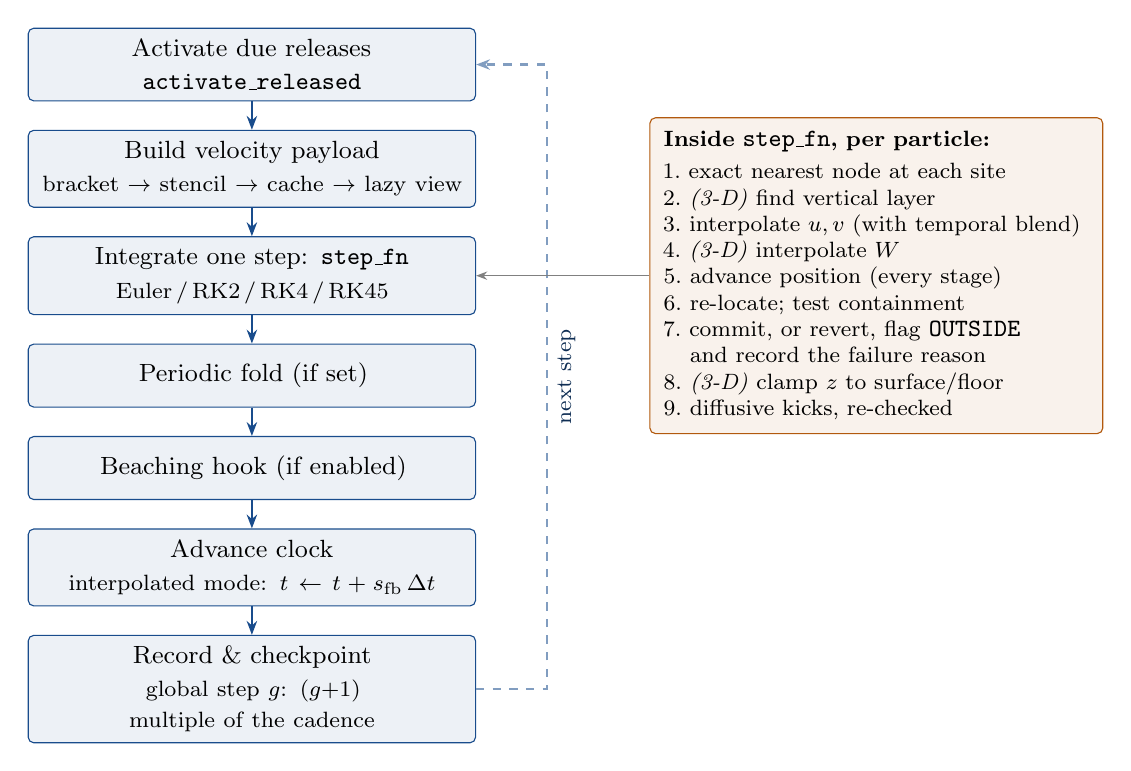
\begin{tikzpicture}[node distance=3.6mm and 16mm,flowbox/.append style={text width=54mm},sidebox/.append style={text width=54mm}]
  \node[flowbox] (act)   {Activate due releases\\[1pt]\code{activate\_released}};
  \node[flowbox,below=of act]   (vel)   {Build velocity payload\\[1pt]\footnotesize bracket $\rightarrow$ stencil $\rightarrow$ cache $\rightarrow$ lazy view};
  \node[flowbox,below=of vel]   (int)   {Integrate one step: \code{step\_fn}\\[1pt]\footnotesize Euler\,/\,RK2\,/\,RK4\,/\,RK45};
  \node[flowbox,below=of int]   (fold)  {Periodic fold (if set)};
  \node[flowbox,below=of fold]  (beach) {Beaching hook (if enabled)};
  \node[flowbox,below=of beach] (clock) {Advance clock\\[1pt]\footnotesize interpolated mode: $t\leftarrow t+\tdir\,\dt$};
  \node[flowbox,below=of clock] (rec)   {Record \& checkpoint\\[1pt]\footnotesize global step $g$: $(g{+}1)$ multiple of the cadence};

  \draw[flowarrow] (act)--(vel);
  \draw[flowarrow] (vel)--(int);
  \draw[flowarrow] (int)--(fold);
  \draw[flowarrow] (fold)--(beach);
  \draw[flowarrow] (beach)--(clock);
  \draw[flowarrow] (clock)--(rec);
  \draw[looparrow] (rec.east) -- ++(0.9,0) |- node[pos=0.25,sloped,below,font=\footnotesize,text=lagblue!60!black]{next step} (act.east);

  \node[sidebox,right=22mm of int] (sub) {%
    \textbf{Inside \code{step\_fn}, per particle:}\\[2pt]
    1.\ exact nearest node at each site\\
    2.\ \emph{(3-D)} find vertical layer\\
    3.\ interpolate $u,v$ (with temporal blend)\\
    4.\ \emph{(3-D)} interpolate $\Wvel$\\
    5.\ advance position (every stage)\\
    6.\ re-locate; test containment\\
    7.\ commit, or revert, flag \code{OUTSIDE}\\
    \phantom{7.\ }and record the failure reason\\
    8.\ \emph{(3-D)} clamp $\depx$ to surface/floor\\
    9.\ diffusive kicks, re-checked};
  \draw[-{Stealth[length=4pt]},gray] (sub.west) -- (int.east);
\end{tikzpicture}
\caption{The per-step pipeline executed by \fn{run\_single\_realization}. The main loop (left) activates any
particles whose release time has arrived, assembles the velocity for the step, integrates, folds particles
back into periodic windows, applies the optional beaching hook, advances the clock, and records and
checkpoints at the configured cadence. The side panel lists the operations performed for each particle
inside the integration step; stages marked \emph{(3-D)} are present only in three-dimensional runs.}
\label{fig:pipeline}
\end{figure}

At each step the engine performs the sequence shown in \cref{fig:pipeline}. It first activates any particles
whose scheduled release time has arrived, so that they are advected during the same step
(\cref{ch:lifecycle}). It then assembles the velocity payload for the step: the stored snapshots that bracket
the current time are identified, the reconstruction stencil is resolved (two snapshots for linear
reconstruction, four for monotone piecewise-cubic), the snapshots are taken from the cache or read, and the
step receives either a snapshot or a lazy view that blends a field only when it is read, together with the
target snapshot for the Runge--Kutta stages (\cref{sec:temp-linear,sec:input-payload}). On a sigma mesh the
surface elevation at the start and the end of the step is supplied as well (\cref{sec:vert-sigma-step}). The
integration step is invoked once; the operations it performs for each particle are listed in the side panel
of \cref{fig:pipeline} and are the subject of \crefrange{ch:localization}{ch:integration}. Particles that left
a periodic window are folded back, and if beaching is enabled a post-step hook evaluates the stranding and
resuspension criteria (\cref{ch:lifecycle}). In the interpolated mode the clock advances by $\tdir\,\dt$; in the
discrete mode the snapshot index advances by $\tdir$, one record forward or backward. The state is recorded, and checkpointed, after every step
whose global index $g$ satisfies that $g+1$ is a multiple of \conf{output\_freq}, respectively
\conf{checkpoint\_freq}, so that a resumed run records the same steps as an uninterrupted one
(\cref{ch:output}); one more checkpoint follows the last executed step. A record is labelled with the time at
the end of its step, samples the requested scalars at that time, un-rotates positions and velocities to
geographic coordinates, writes the rows of not-yet-released particles as missing values, and writes the
velocity as missing wherever the particle was not alive through the whole step.

The boundary conditions are applied inside the step, immediately after the position is advanced. The
containing-element test serves as the domain check: a particle whose new position is not contained by any
element --- whether it has crossed an open boundary or left a coastline --- has its step undone and its status
set to \code{OUTSIDE}. Vertical limits, by contrast, are enforced by clamping rather than removal: a particle
that would cross the surface or the local sea floor is held at that limit (\cref{ch:vertical,ch:lifecycle}).
With the option \code{-v} the loop prints, per step, the time spent reading (\code{io=}), stepping
(\code{step=}), beaching (\code{beach=}) and recording (\code{rec=}) (\cref{sec:perf-measure}).

\codeanchor{The step sequence is the loop body of \fn{run\_single\_realization}
(\srcfile{tracking.py}); the per-particle operations are implemented in the
integration kernels of \srcfile{numerics/integrators.py}.}

\section{Forward and backward integration}\label{sec:arch-direction}

The engine integrates equally in either time direction, and it does so without a
separate backward code path. The direction factor $\tdir\in\{+1,-1\}$ is folded
into the interpolated velocity: every interpolation routine returns
$\tdir\,u$, $\tdir\,v$ and $\tdir\,\Wvel$ rather than the raw model velocity, while
the time step $\dt$ remains positive. Backward integration is therefore a sign
reversal of the sampled velocity, and the same integrator advances the position in
both cases. The step counter increments in both directions, and the simulation
clock advances by $\tdir\,\dt$. With stochastic diffusion the backward run is the adjoint process: the
advection is reversed, the diffusive drift and noise are not (\cref{sec:diff-model}). This symmetry is what the reversibility tests of
\cref{ch:validation} exploit: integrating forward and then backward over the same
interval, with the same scheme, returns a particle to its starting point to within
a small tolerance.

\section{Fused and unfused execution paths}\label{sec:arch-fused}

The per-particle operations of \cref{fig:pipeline} are realized by two interchangeable implementations. A set
of \emph{fused} kernels, compiled just-in-time, performs the whole step --- localization, interpolation,
integration and the boundary check --- within a single compiled loop over the particles, for the common
configurations to which they apply: two-dimensional least-squares runs, time-dependent two-dimensional
barycentric runs on node velocities (RK2 and RK4, linear interpolation in time, no element tracking), three-dimensional Euler with least-squares velocities on z-level meshes (vertical combine \conf{nearest}
or \conf{leastsq}), and
three-dimensional RK2 with node-layout barycentric velocities when the vertical velocity is combined by
\conf{nearest} or \conf{barycentric}. An \emph{unfused} path performs the same operations as separate parallel
passes over all particles and covers every other configuration. Where both exist they produce bit-for-bit
identical trajectories, statuses and failure reasons under the default exact anchor guard
(\conf{mesh.exact\_nearest}); the details are in \cref{ch:fused}.


\part{Mesh and Localization}
\chapter{The Unstructured Mesh}\label{ch:mesh}

This chapter describes the static geometry on which the engine operates: the
unstructured mesh, the quantities a model stores on it, and the conventions under which each source ---
FESOM2, FESOM~1.4, FESOM-C, HEALPix products and structured NEMO grids --- is read into the \fn{Mesh} structure of
\cref{sec:arch-data}. We use the triangular FESOM2 \emph{core2} mesh as the worked example and describe
the other sources where they differ. The localization search of \cref{ch:localization} and every
interpolation stencil of \crefrange{ch:hvel}{ch:sampling} are expressed in terms of
the entities introduced here, so we also fix the vocabulary --- node, element,
interface, layer --- used throughout the manual.

\section{Nodes, elements, and interfaces}\label{sec:mesh-anatomy}

The horizontal mesh is a tessellation of the ocean surface: a set of $N$
\emph{nodes} joined into $E$ \emph{elements}. \index{node}\index{element} In FESOM2
the elements are triangles; in FESOM-C they are mixed, each element being a triangle
or a quadrilateral; structured grids and the HEALPix pixel mesh produce quadrilaterals only, and the
HEALPix dual mesh quadrilaterals with a few triangles (\cref{sec:mesh-sources}). A triangle in a mesh with room for four vertices is stored with its fourth slot
set to $-1$.
For the FESOM2 \emph{core2} configuration used as the running example the elements are
triangular, with $N=\num{126858}$ nodes and $E=\num{244659}$ elements. Each element
stores the indices of its vertices --- three for a triangle, four for a quadrilateral
--- and the engine precomputes, for each node, the list of elements that contain it
(its \emph{one-ring}), which the localization search relies upon
(\cref{ch:localization}).

The model does not store all fields at the same location, and the distinction is
fundamental to interpolation (\cref{fig:mesh-anatomy}). \emph{Node-layout} fields
are defined at the vertices: the FESOM2 horizontal velocity components \conf{unod}
and \conf{vnod}, the sea-surface height, and the sampled scalars (temperature,
salinity) are all node quantities. \emph{Element-layout} fields are defined at the
element centroids: the alternative monthly-mean FESOM2 velocities \conf{u} and
\conf{v} are element quantities. A node-layout field carries one value per vertex
and is interpolated by the barycentric scheme of \cref{ch:hvel}; an element-layout
field carries one value per element and is interpolated by either least-squares scheme or,
through area-weighted vertex values, the barycentric scheme of the same chapter. The \fn{VelocityField} records which layout applies in
its \code{uv\_layout} attribute, and the engine selects the matching stencil
accordingly.

\begin{figure}[t]
\centering
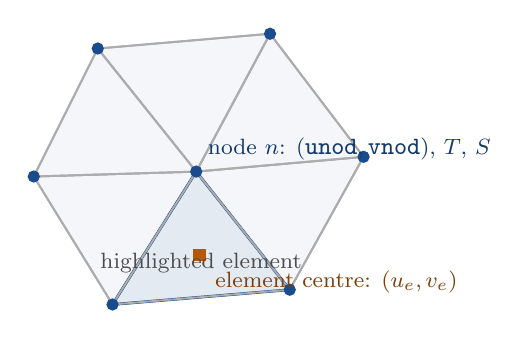
\begin{tikzpicture}[scale=1.25]
  \coordinate (C)  at (2.00,1.55);
  \coordinate (p1) at (0.35,1.50);
  \coordinate (p2) at (1.15,0.20);
  \coordinate (p3) at (2.95,0.35);
  \coordinate (p4) at (3.70,1.70);
  \coordinate (p5) at (2.75,2.95);
  \coordinate (p6) at (1.00,2.80);
  % the one-ring of triangles around node C
  \foreach \a/\b in {p1/p2,p2/p3,p3/p4,p4/p5,p5/p6,p6/p1}
     \fill[meshface] (C)--(\a)--(\b)--cycle;
  % highlight one element
  \fill[hilface] (C)--(p2)--(p3)--cycle;
  \foreach \a/\b in {p1/p2,p2/p3,p3/p4,p4/p5,p5/p6,p6/p1}{
     \draw[meshedge] (C)--(\a); \draw[meshedge] (\a)--(\b);}
  % element centroid of (C,p2,p3)
  \node[elemcentre] (E) at ($ 0.3333*(C) + 0.3333*(p2) + 0.3333*(p3) $) {};
  % nodes
  \foreach \p in {C,p1,p2,p3,p4,p5,p6} \node[meshnode] at (\p) {};
  % labels
  \node[nodelbl,above right=1pt of C] {node $n$: $(\conf{unod},\conf{vnod})$, $T$, $S$};
  \node[elemlbl,below right=0pt of E] {element centre: $(u_e,v_e)$};
  \node[font=\footnotesize,gray!60!black] at (2.05,0.62) {highlighted element};
\end{tikzpicture}
\caption{Anatomy of the horizontal mesh. Triangle vertices are \emph{nodes}
(filled circles), where node-layout velocities and the scalar fields live; triangle
centroids are \emph{elements} (the orange square), where element-layout velocities
live. The six shaded triangles sharing the central node $n$ form its one-ring, the
adjacency the localization search exploits (\cref{ch:localization}).}
\label{fig:mesh-anatomy}
\end{figure}

\section{Vertical structure: interfaces and layers}\label{sec:mesh-vertical}

In the vertical, the water column is divided by $K$ \emph{interfaces} into $K-1$
\emph{layers} (\cref{fig:mesh-column}). \index{interface}\index{layer} The
interfaces are the level boundaries; the layers are the volumes between them. The
distinction matters because, again, different fields live in different places: the
vertical velocity $\Wvel$ is defined \emph{at the interfaces}, whereas the
three-dimensional horizontal velocity and the scalar fields are defined \emph{at
the mid-layers}. FESOM~1.4 is the exception: it stores every field on the levels, so its horizontal
velocity shares the interfaces with $\Wvel$ (\cref{sec:mesh-fesom14}). For the \emph{core2} mesh there are $48$ interfaces and hence $47$
layers, spanning depths from $0$ to approximately \SI{6250}{\metre}. The
configuration key \conf{max\_levels} retains only the first $N$ interfaces from the
surface downward (at least two in three dimensions, on either vertical family), which both saves memory
and caps the depth a particle can reach; a run that follows water to the sea floor keeps the full
column.

\begin{figure}[t]
\centering
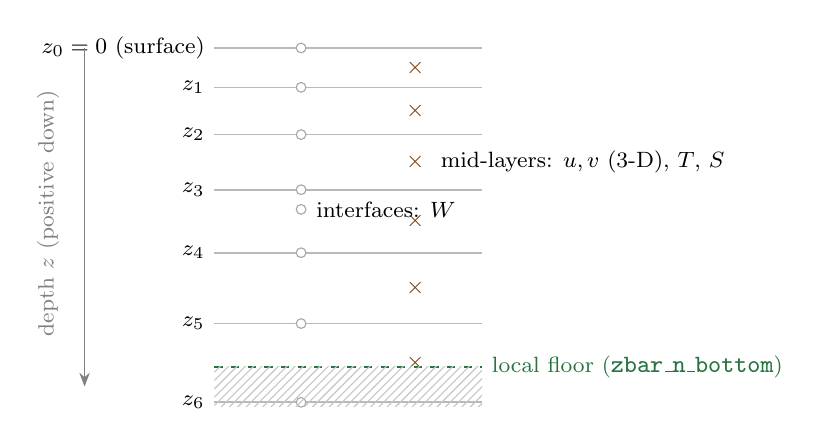
\begin{tikzpicture}[scale=1.0]
  \def\xa{0} \def\xb{3.4}
  % interface depths (increasing layer thickness with depth)
  \foreach \y/\lab in {0/{$z_0=0$ (surface)},-0.5/{$z_1$},-1.1/{$z_2$},-1.8/{$z_3$},-2.6/{$z_4$},-3.5/{$z_5$}}{
     \draw[interface] (\xa,\y)--(\xb,\y);
     \node[interfacept] at (1.1,\y) {};
     \node[font=\footnotesize,left] at (\xa,\y) {\lab};
  }
  \draw[interface] (\xa,-4.5)--(\xb,-4.5);
  \node[interfacept] at (1.1,-4.5) {};
  \node[font=\footnotesize,left] at (\xa,-4.5) {$z_6$};
  % mid-layer markers
  \foreach \y in {-0.25,-0.8,-1.45,-2.2,-3.05,-4.0}
     \node[font=\footnotesize,lagelem!70!black] at (2.55,\y) {$\times$};
  % local sea floor
  \draw[dashed,laggreen,line width=0.9pt] (\xa,-4.05)--(\xb,-4.05);
  \node[font=\footnotesize,laggreen,right] at (\xb,-4.05) {local floor (\conf{zbar\_n\_bottom})};
  \fill[pattern=north east lines,pattern color=gray!45] (\xa,-4.05) rectangle (\xb,-4.55);
  % depth axis
  \draw[-{Stealth[length=5pt]},gray] (-1.65,0.0)--(-1.65,-4.3);
  \node[gray,rotate=90,anchor=south,font=\footnotesize] at (-1.85,-2.1) {depth $\depx$ (positive down)};
  % field-location annotations
  \node[font=\footnotesize,interfacept,label={[font=\footnotesize]right:{interfaces: $\Wvel$}}] at (1.1,-2.05) {};
  \node[font=\footnotesize,lagelem!70!black] at (2.55,-2.62) {};
  \node[font=\footnotesize,right] at (2.75,-1.45) {mid-layers: $u,v$ (3-D), $T$, $S$};
\end{tikzpicture}
\caption{Anatomy of the vertical column. The $K$ interfaces (grey lines, open
circles) bound $K-1$ mid-layers (orange crosses). The vertical velocity $\Wvel$ is
stored at the interfaces; the three-dimensional horizontal velocity and the scalar
fields are stored at the mid-layers. The local sea floor is given per node by
\conf{zbar\_n\_bottom}; layers below it do not exist for that node and a particle
cannot descend past it (\cref{ch:vertical}).}
\label{fig:mesh-column}
\end{figure}

The engine treats FESOM2 levels as fixed depths (a \emph{z-level} vertical coordinate), the same
everywhere. In FESOM2 itself the interfaces follow the free surface (the zstar coordinate), and the
recorded depth is therefore the reference depth, within $|\eta|$ of the physical one
(\cref{sec:vert-wsign}).
The alternative supported family, used by the FESOM-C model, is a
terrain-following \emph{sigma} coordinate in which the interface depths are a
fixed fraction of the local water-column thickness and therefore vary in space and
with the sea-surface height. The two families differ only in how an interface depth
is computed; we defer the sigma geometry to \cref{ch:vertical}. FESOM~1.4, HEALPix products and NEMO
grids use z-levels.

\section{Reading a mesh file}\label{sec:mesh-conventions}

The FESOM2 reader accepts three mesh sources: a mesh-diagnostics NetCDF file, an ASCII mesh directory, and
a Zarr store written by the region-extraction tool. It resolves the quantities of a diagnostics file by
variable \emph{name} rather than by dimension, which lets it read three naming conventions --- node
coordinates as \code{lon}/\code{lat} in degrees or packed as one \code{nodes} array in radians, and the
connectivity as \code{elements}, \code{elem} or \code{face\_nodes}, oriented to $(E,3)$ by its axis of
length three --- and applies a small number of unit and indexing conversions (\cref{tab:mesh-vars}). Packed
coordinates are converted to degrees, trusting an explicit \code{units} attribute when present and otherwise
inferring radians when the longitude magnitude does not exceed $2\pi$ and the latitude magnitude does not
exceed $\pi/2$. The connectivity is shifted to zero-based indexing by its \code{start\_index} attribute
(one, as FESOM2 writes it from Fortran, when absent). Depth-like quantities --- the interface levels and the
per-node sea-floor depth --- are stored with a negative-downward sign and are converted to the positive-down
convention by taking absolute values. Element centres are computed from the vertices, with the longitude
averaged on the circle so that an element across the dateline gets a centre inside it. The model's element
areas are kept when the file provides them.

\begin{table}[t]
\centering
\caption{Quantities read from the FESOM2 mesh-diagnostic file and their conversion
to the \fn{Mesh} structure.}
\label{tab:mesh-vars}
\small
\begin{tabularx}{\linewidth}{@{}l l X@{}}
\toprule
File variable & \fn{Mesh} member & Conversion / convention \\
\midrule
\code{lon}, \code{lat} or \code{nodes} $(2,N)$ & \code{nodes\_lon/lat} & degrees; packed radians $\rightarrow$ degrees \\
\code{elements}, \code{elem} or \code{face\_nodes} & \code{elem\_nodes}    & oriented to $(E,3)$; one-based $\rightarrow$ zero-based \\
\code{nz} or \code{zbar}    & \code{sigma}, \code{z\_levels} & $|\cdot|$, positive-down interface depths \\
\code{zbar\_n\_bottom}      & \code{depth}          & $|\cdot|$, per-node sea floor (positive-down) \\
\code{elem\_area}           & element areas         & used directly when present \\
\code{nod\_in\_elem2D} (+ count) & \code{node\_to\_elems} & one-based $\rightarrow$ zero-based; rebuilt if degenerate (\cref{sec:mesh-nodeelem}); required in a diagnostics file \\
\code{zbar\_e\_bottom}, \code{nlevels} & element bottoms (metadata) & each element's bed and last whole layer, when present (\cref{sec:mesh-elem-bottoms}) \\
\code{ulevels}             & element first levels (metadata) & above 1 under an ice-shelf cavity \\
\bottomrule
\end{tabularx}
\end{table}

\codeanchor{Mesh-variable resolution and conversions are in \fn{\_resolve\_mesh\_vars},
\fn{\_load\_mesh\_nc} and \fn{\_compute\_elem\_centres} (\srcfile{readers/fesom2.py}); the \fn{Mesh}
dataclass and its \code{z\_levels} property are in \srcfile{core/mesh.py}.}

\section{The node-to-element table and its reconstruction}\label{sec:mesh-nodeelem}

The localization search requires, for each node, the list of elements that contain
it; this is the \code{nod\_in\_elem2D} table in the mesh file. On the \emph{core2}
mesh this table is effectively empty: of the $\num{733977}$ node--element incidences it should hold
(three per element) only $54$ are present. \index{nod\_in\_elem2D@\code{nod\_in\_elem2D}} The consequence, if the
table were used as read, is severe and silent. After the routine one-based to
zero-based shift, every unpopulated entry becomes $-1$, so that $\num{126852}$ of
the $\num{126858}$ nodes report no adjacent elements. The containing-element search
of \cref{ch:localization} would then fail for every particle on the first step,
flag each as having left the domain, and terminate normally --- producing an output
file in which no particle ever moved, with no error raised.

To prevent this, the reader detects a degenerate table and rebuilds it from the
element connectivity, which is intact. The detector flags the table as degenerate on
any of three independent signals: more than half of the nodes report no first
element; an entry strictly inside a node's declared neighbour count is empty (the
table and the count array disagree); or a neighbour count is negative or exceeds the
maximum connectivity. On a positive verdict the engine prints a notice and
reconstructs the node-to-element adjacency by a two-pass count-and-fill over the
elements, after which the localization search behaves correctly. We note this
behaviour explicitly because it is a precondition for any meaningful run on the
\emph{core2} mesh, and because its failure mode --- a completed run with no motion
--- is easy to misread as a physical result rather than a missing table.

\codeanchor{The degeneracy detector \fn{\_nod\_in\_elem2d\_is\_degenerate} and the
rebuild call are in \srcfile{readers/fesom2.py}; the reconstruction
\fn{build\_node\_to\_elems} (a two-pass count-and-fill) is in \srcfile{core/mesh.py}.}

\section{Element bottoms}\label{sec:mesh-elem-bottoms}

FESOM2 fixes the number of levels of each element first and gives a node the deepest of the elements
around it, so the per-node floor \code{zbar\_n\_bottom} tells where the deepest element at a node ends,
not where a given element ends. The depth-linear reading of element-layout velocities
(\cref{sec:vert-uvdepth}) needs the bed of every element, and the FESOM2 reader takes it from the mesh
diagnostic --- NetCDF or Zarr --- when the diagnostic holds the element level variables: \code{nlevels}
(one-based; the element has $\code{nlevels}-1$ wet layers), \code{zbar\_e\_bottom} (its bed, negative
down) and \code{ulevels} (its first level, above 1 under an ice-shelf cavity). From them it declares, in
file element order, the bed $d_e$ and the last whole layer $D_e$ of each element,
\begin{equation}\label{eq:mesh-elem-bed}
  d_e = \begin{cases} |\code{zbar\_e\_bottom}_e| & \text{when present},\\
                      z_{\code{nlevels}_e-1} & \text{otherwise},\end{cases}
  \qquad
  D_e = \max\{k : z_{k+1}\le d_e\}\quad(-1 \text{ when } z_1>d_e),
\end{equation}
that is, the last layer whose lower level lies at or above the bed. A bottom layer that the bed cuts ---
a FESOM2 \emph{partial bottom cell} --- is therefore not counted, and the depth-linear rule never reads it,
the same rule as the node table of \cref{eq:vert-uv-last}. The element first levels are kept as well.
A variable read here that is not one finite value per element, or that holds levels outside $1,\dots,K$,
refuses the mesh at load --- in layer runs too --- with a message that names the file and the fix, and
the loader prints one line saying whether the bottoms came from the file. A mesh without either
variable --- an ASCII mesh directory, a diagnostic that lacks them, a Zarr store without a level table, or
a region extracted before the extraction tool kept them --- declares no bottoms, and
\conf{mode.uv\_vertical: linear} on its element velocities is refused before the output file exists;
\code{ulevels} alone declares nothing. A mesh with \code{ulevels}${}>1$ anywhere is refused for the
same option: ice-shelf cavities are not supported in the code yet and are planned. The region-extraction
tool \code{utils/extract\_fesom\_region.py} writes \code{nlevels}, \code{ulevels} and
\code{zbar\_e\_bottom} of the kept elements, and \code{nlevels\_nod2D} of the kept nodes, whenever the
source has them, with the values and signs of the source; a subset written before it did so must be
extracted again to use the option on element data.

\codeanchor{\raggedright \fn{\_elem\_level\_metadata} in \srcfile{readers/fesom2.py}, called by the NetCDF and the Zarr
mesh loaders, declares \code{mesh.metadata["elem\_bed"]}, \code{["uv\_data\_last\_elem"]},
\code{["elem\_ulevels"]} and \code{["elem\_levels\_source"]}; the element table that reads them is
\fn{depth\_points} with \code{layout="element"} (\srcfile{numerics/vertical\_uv.py}); the subset writer is
\srcfile{utils/extract\_fesom\_region.py}.}


\section{Other mesh sources}\label{sec:mesh-sources}

The other readers produce the same \fn{Mesh} from different inputs (\cref{tab:mesh-sources,fig:mesh-sources});
the FESOM~1.4 reader has a section of its own (\cref{sec:mesh-fesom14}).

\begin{table}[t]
\centering\footnotesize\setlength{\tabcolsep}{4pt}
\begin{tabular}{@{}>{\raggedright\arraybackslash}p{23mm}>{\raggedright\arraybackslash}p{29mm}>{\raggedright\arraybackslash}p{29mm}>{\raggedright\arraybackslash}p{17mm}>{\raggedright\arraybackslash}p{16mm}>{\raggedright\arraybackslash}p{14mm}@{}}
\toprule
source & nodes & elements & velocity layout & vertical & radius (m) \\
\midrule
FESOM2 & model nodes & triangles & node or element & z-level & \num{6367500} \\
FESOM~1.4 & model nodes & triangles, from the mesh files or the cell polygons & node, on the levels & z-level & \num{6367500} \\
FESOM-C & model nodes & triangles, quadrilaterals & element (node when stored so) & sigma & \num{6400000} \\
HEALPix, dual & wet pixel centres & corner cells: quadrilaterals, some triangles & node & z-level & \num{6371000} \\
HEALPix, pixel & pixel corners & wet pixels (quadrilaterals) & element & two-dim. & \num{6371000} \\
NEMO & wet T-points & quadrilaterals of four wet T-points & node & two-dim. & \num{6371000} \\
\bottomrule
\end{tabular}
\caption{Mesh sources. The radius is the default of \conf{mesh.r\_earth}; it enters the fallback
computation of element areas and, without effect on the values, the barycentric projection.}
\label{tab:mesh-sources}
\end{table}

\paragraph{FESOM-C.} The FESOM-C reader takes the node coordinates, depths and vertex lists from the
model's single output file, together with the element centres when present and the sigma levels. Its
connectivity is sanitised on load: indices are shifted to zero-based, empty and repeated vertices are
removed, and each row is compacted, so a triangle stored as a quadrilateral with a repeated vertex
becomes $[a,b,c,-1]$.

\paragraph{HEALPix, dual mesh.} A HEALPix product stores its fields at the centres of equal-area pixels.
The default \emph{dual} mesh takes the wet pixel centres as nodes and builds one element around each pixel
corner, joining the pixels that meet there: four pixels give a quadrilateral, and at the eight points of
the sphere where only three pixels meet, a triangle. The cells are built from the pixel neighbour
relations in integer arithmetic, each kept once; an all-wet sphere must give exactly two more elements than
pixels, which the builder checks. A pixel is wet when the velocity at the first record is finite on the
tracked level, restricted by \conf{mesh.crop\_bbox} and by a bathymetry variable when the store has one.
The velocities live at the nodes, so the dual mesh needs \conf{uv\_interp: barycentric}.

\paragraph{HEALPix, pixel mesh.} With \conf{mesh.healpix\_geometry: pixel} the elements are the wet pixels
themselves, quadrilaterals whose nodes are the pixel corners; the velocities live at the element centres,
so both least-squares schemes apply. A quadrilateral with straight edges approximates a pixel with curved
edges, so near an edge a point may be assigned to the adjacent pixel. The pixel mesh is two-dimensional;
the eight pixels that touch a pole are degenerate in the geographic frame and produce a warning.

\paragraph{Structured grids and NEMO.} A logically rectangular grid becomes a mesh of quadrilaterals whose
corners are four adjacent wet cell centres (T-points); a quadrilateral with a land corner is dropped, which
draws the coastline, and a wet T-point that belongs to no quadrilateral is left out, since it could only be
a dead end. The NEMO reader averages the C-grid velocities at the cell faces to the T-points, setting
missing face values to zero first, which gives node-layout velocities. Its first version is two-dimensional
and requires a grid whose axes are within $2^\circ$ of east and north.

\begin{figure}[t]
\centering
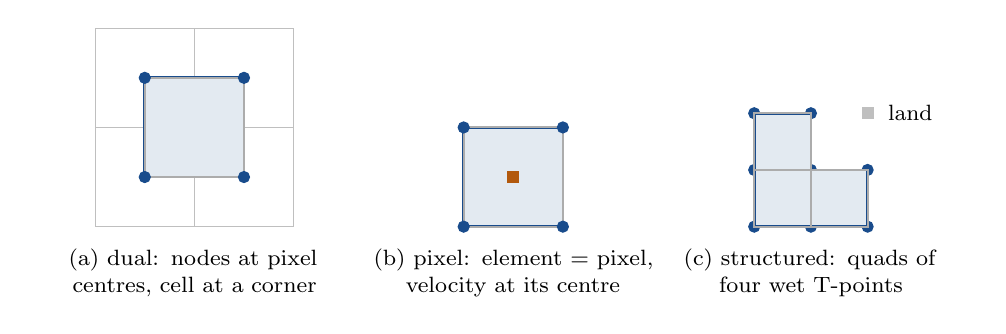
\begin{tikzpicture}[scale=0.9]
  % (a) HEALPix dual: pixel centres as nodes, a quad around a 4-valent corner, a triangle around a 3-valent one
  \begin{scope}
    \foreach \x/\y in {0/0,1.4/0,0/1.4,1.4/1.4} \draw[gray!50] (\x-0.7,\y-0.7) rectangle (\x+0.7,\y+0.7);
    \fill[hilface] (0,0)--(1.4,0)--(1.4,1.4)--(0,1.4)--cycle;
    \draw[meshedge] (0,0)--(1.4,0)--(1.4,1.4)--(0,1.4)--cycle;
    \foreach \x/\y in {0/0,1.4/0,0/1.4,1.4/1.4} \node[meshnode] at (\x,\y) {};
    \node[font=\footnotesize,align=center,text width=40mm] at (0.7,-1.35) {(a) dual: nodes at pixel\\centres, cell at a corner};
  \end{scope}
  % (b) pixel mesh: pixel as element, corners as nodes
  \begin{scope}[xshift=5.2cm]
    \fill[hilface] (-0.7,-0.7) rectangle (0.7,0.7);
    \draw[meshedge] (-0.7,-0.7) rectangle (0.7,0.7);
    \foreach \x/\y in {-0.7/-0.7,0.7/-0.7,0.7/0.7,-0.7/0.7} \node[meshnode] at (\x,\y) {};
    \node[elemcentre] at (0,0) {};
    \node[font=\footnotesize,align=center,text width=40mm] at (0,-1.35) {(b) pixel: element = pixel,\\velocity at its centre};
  \end{scope}
  % (c) structured grid: T-point quads, one land cell
  \begin{scope}[xshift=8.6cm,yshift=-0.7cm]
    \foreach \i in {0,1,2} \foreach \j in {0,1,2} {
      \ifnum\i=2 \ifnum\j=2 \else \node[meshnode] at (\i*0.8,\j*0.8) {};\fi \else \node[meshnode] at (\i*0.8,\j*0.8) {};\fi }
    \fill[hilface] (0,0) rectangle (0.8,0.8);
    \fill[hilface] (0.8,0) rectangle (1.6,0.8);
    \fill[hilface] (0,0.8) rectangle (0.8,1.6);
    \draw[meshedge] (0,0) rectangle (0.8,0.8) (0.8,0) rectangle (1.6,0.8) (0,0.8) rectangle (0.8,1.6);
    \node[rectangle,fill=gray!50,inner sep=2.2pt] at (1.6,1.6) {};
    \node[font=\footnotesize,anchor=west] at (1.75,1.6) {land};
    \node[font=\footnotesize,align=center,text width=40mm] at (0.8,-0.65) {(c) structured: quads of\\four wet T-points};
  \end{scope}
\end{tikzpicture}
\caption{Three mesh sources on one \fn{Mesh}. (a) The HEALPix dual mesh joins the four pixel centres around
a pixel corner into a quadrilateral (three centres give a triangle). (b) The pixel mesh makes each wet pixel
an element, with nodes at its corners and the velocity at its centre. (c) A structured grid keeps the
quadrilaterals whose four T-points are wet; one land point removes the quadrilateral in the corner.}
\label{fig:mesh-sources}
\end{figure}

\codeanchor{\fn{\_sanitize\_connectivity} and \fn{FesomCReader.load\_mesh} (\srcfile{readers/fesomc.py});
\fn{build\_healpix\_dual\_mesh}, \fn{build\_healpix\_pixel\_mesh} and \fn{HealpixReader.load\_mesh}
(\srcfile{readers/healpix.py}); \fn{build\_structured\_mesh} and \fn{c\_grid\_to\_t}
(\srcfile{readers/structured.py}); the NEMO adapter in \srcfile{readers/nemo.py}.}

\section{The FESOM~1.4 mesh}\label{sec:mesh-fesom14}

FESOM~1.4 \citep{wang2014fesom14} is a finite-element model on a triangular surface mesh that is the same
at every level. Every surface node has a column of three-dimensional nodes, one per level, down to its
bed, and all prognostic fields --- $u$, $v$, $\Wvel$, temperature and salinity --- are continuous,
piecewise-linear (P1) functions on the tetrahedra between those nodes: they live \emph{on the levels at the
nodes}. The reader therefore returns node-layout fields on the levels (\cref{sec:vert-uvdepth}), and it
builds the \fn{Mesh} from either of two sources, decided by what \conf{mesh.meshpath} is.

\paragraph{ASCII mesh directory.} A directory that holds \code{nod3d.out} is read as the model's mesh
files: \code{nod2d.out} (the node coordinates and flags), \code{elem2d.out} (the triangles, one-based),
\code{nod3d.out} (every three-dimensional node with its depth, numbered level by level) and
\code{aux3d.out} in FESOM~1.4's own format --- the number of levels, the table of the three-dimensional
node at each level of each column (a value $\le0$ marks a dry slot) and the surface node of every
three-dimensional node; its last block, on the three-dimensional elements, is not parsed. This
\code{aux3d.out} is not FESOM2's, and the FESOM2 reader would misread it. Each file is read as one stream
of numbers, as a Fortran list-directed read sees it, so the spread of the records over lines does not
matter; Fortran \code{D} exponents are accepted, and an integer field takes any number whose value is an
integer. The levels are the depths of \code{nod3d.out} in file order --- every change of value starts a new
level --- stored positive down, with the surface exactly at zero. Before anything is returned the files
are checked against each other: indices in range, every three-dimensional node in exactly one slot, the
wet slots a prefix of each column, and every slot's surface node and depth consistent with the node
tables. A failure names the file and the first offending index.

A FESOM~1.4 run may store its mesh in the rotated frame of the model. The key \conf{mesh.input\_rotation}
takes the Euler angles $[\alpha,\beta,\gamma]$ of the run's namelist, in degrees, and rotates the node
coordinates back to geographic on load, with the convention of \cref{sec:frame-rotation}. The angles are
never guessed, since a rotated mesh looks like a geographic one; the reader warns when a global ASCII mesh
(more than $350^\circ$ of longitude) without a node north of $85^\circ$\,N is loaded without them, because a
geographic FESOM mesh reaches the Arctic. The key is refused for a mesh from cell polygons, whose
coordinates are geographic, and for every other mesh type; it is independent of \conf{mesh.rotation}, the
frame in which the engine tracks (\cref{ch:frame}).

\paragraph{Cell polygons of level-wise data.} Published FESOM~1.4 output, such as the CMIP6 files, holds
no element table. It holds, next to the node coordinates \code{lon}/\code{lat}, each node's
\emph{median-dual cell} as a polygon (\code{lon\_bnds}/\code{lat\_bnds}, padded to a fixed vertex count by
repeating the last vertex). An interior node's polygon alternates the midpoints of its edges and the
centroids of its triangles; a coastal node's polygon also holds the midpoints of its boundary edges and the
node itself. A polygon vertex shared by exactly three nodes is therefore the centroid of their triangle
(\cref{fig:mesh-fesom14}), and the reader recovers the triangles exactly from that rule. The polygon
vertices of all nodes are clustered on the unit sphere within $10^{-6}$ degrees (about \SI{0.1}{\metre});
distinct clusters must lie at least a thousand times farther apart, so that no point split by rounding can
pass for two. At a \emph{pinch node}, whose triangles form several fans that touch only at the node, the
published polygon lists one fan only; a centroid listed by just two nodes then names its third node, and
that triangle is recovered as well. The result is validated before it is used: a shared point within
\SI{1}{\centi\metre} of the spherical centroid of its three nodes, every edge in one or two triangles with a
polygon vertex at its midpoint, the Euler characteristic $V-E+F=2C-L$ of $C$ edge-connected components with
$L$ boundary loops, and an accounting check that every distinct polygon vertex is a node, the midpoint of a
recovered edge or the centroid of a recovered triangle. The levels are the file's depth coordinate (finite,
starting at the surface, increasing), and the wet mask comes from the first record of $u$: a value counts
as data when it is finite and smaller than $10^{29}$ in magnitude, and the data of every column must be a
prefix of its levels, starting at the surface. When a file holds \code{deptho} (for instance the published
fixed-field file in the same directory), its value must equal the depth of each column's last level with
data within \SI{0.01}{\metre}. This is the only guard against level-wise files that write zero rather than
a fill value below the bed, whose first record would look wet everywhere; without \code{deptho} that case
cannot be detected.

\begin{figure}[t]
\centering
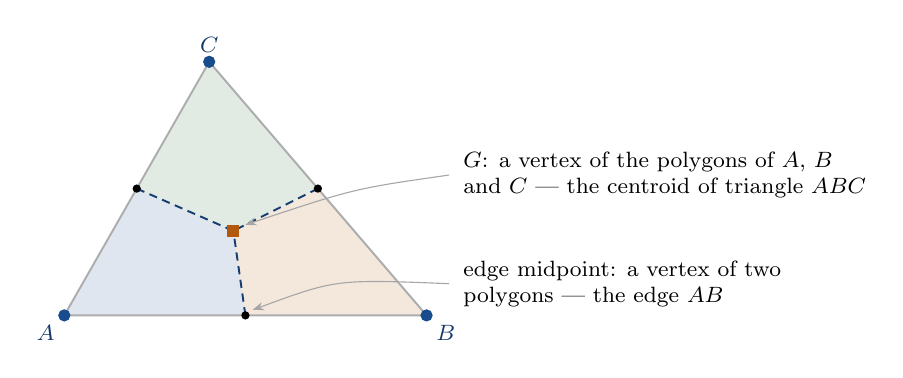
\begin{tikzpicture}[scale=1.15]
  \coordinate (A) at (0,0); \coordinate (B) at (4,0); \coordinate (C) at (1.6,2.8);
  \coordinate (G) at (1.8667,0.9333);
  \coordinate (Mab) at (2,0); \coordinate (Mbc) at (2.8,1.4); \coordinate (Mca) at (0.8,1.4);
  \fill[lagnode!14] (A)--(Mab)--(G)--(Mca)--cycle;
  \fill[lagelem!14] (B)--(Mbc)--(G)--(Mab)--cycle;
  \fill[laggreen!14] (C)--(Mca)--(G)--(Mbc)--cycle;
  \draw[meshedge] (A)--(B)--(C)--cycle;
  \draw[lagnode!80!black,densely dashed,line width=0.7pt] (Mab)--(G) (Mbc)--(G) (Mca)--(G);
  \foreach \p in {A,B,C} \node[meshnode] at (\p) {};
  \foreach \p in {Mab,Mbc,Mca} \node[circle,fill=black,inner sep=0pt,minimum size=3pt] at (\p) {};
  \node[elemcentre] at (G) {};
  \node[nodelbl,below left] at (A) {$A$};
  \node[nodelbl,below right] at (B) {$B$};
  \node[nodelbl,above] at (C) {$C$};
  \node[font=\footnotesize,anchor=west,align=left] at (4.3,1.55) {$G$: a vertex of the polygons of $A$, $B$\\and $C$ --- the centroid of triangle $ABC$};
  \draw[gray!70,-{Stealth[length=4pt]}] (4.25,1.55)..controls (3.2,1.4)..(2.0,1.0);
  \node[font=\footnotesize,anchor=west,align=left] at (4.3,0.35) {edge midpoint: a vertex of two\\polygons --- the edge $AB$};
  \draw[gray!70,-{Stealth[length=4pt]}] (4.25,0.35)..controls (3.0,0.4)..(2.08,0.06);
\end{tikzpicture}
\caption{Triangle recovery from FESOM~1.4 cell polygons. The median-dual cell of each node (shaded, one
colour per node) is bounded by the dashed segments joining the edge midpoints (dots) to the triangle
centroid $G$ (square). Within one triangle each node's cell contributes the quadrilateral node, midpoint,
centroid, midpoint, so $G$ is the only point that the polygons of exactly three nodes share: every cluster
of polygon vertices owned by three nodes is a triangle of the mesh.}
\label{fig:mesh-fesom14}
\end{figure}

\paragraph{The mesh in either case.} \code{mesh.sigma} holds the full level table, positive down, and
\code{mesh.depth} the depth of each column's last wet level, exactly. The reader keeps the static wet mask
of every column (against which every record of every variable is later compared, \cref{sec:input-reader}),
the geographic node coordinates, and the index of each column's last wet level, which it declares as the
data prefix of the depth-linear rule ($D_i$ in \cref{eq:vert-uv-last}). Element centres are circular means
of the vertices, as for FESOM2, and the default radius is \SI{6367500}{\metre}, FESOM~1.4's value. A mesh
whose columns do not all start at the surface --- a mesh with ice-shelf cavities --- is refused by the
reader: an ASCII mesh whose top wet node lies below $z=0$, or level-wise data with a column that holds no
surface value. Ice-shelf cavities are not supported in the code yet and are planned.

\codeanchor{\raggedright The mesh is built by \fn{Fesom14Reader.load\_mesh} in \srcfile{readers/fesom14/reader.py},
with the helpers \fn{\_from\_ascii}, \fn{\_from\_polygons}, \fn{\_check\_deptho} and \fn{\_assemble}
of the same file; the ASCII files are parsed by \fn{read\_ascii\_mesh}
(\srcfile{readers/fesom14/\_ascii\_mesh.py}) and the triangles recovered by \fn{recover\_triangles}
(\srcfile{readers/fesom14/\_polygons.py});
the validity predicate \fn{is\_data} and \fn{wet\_mask\_levelwise} (\srcfile{readers/fesom14/\_layout.py});
the Euler rotation \fn{euler\_matrix} (\srcfile{core/rotation.py}).}


\section{Convex quadrilaterals and derived tables}\label{sec:mesh-derived}

The quadrilateral weights of \cref{sec:hvel-quad} have no fall-back, so every quadrilateral must be convex.
The FESOM-C reader, the structured-grid builder and the HEALPix dual builder check this when the mesh is
loaded (the HEALPix pixel builder too, except for the eight pixels that touch a pole, which it only reports
with a warning): each quadrilateral is projected onto the plane tangent to the sphere at its centre, and it fails
when the cross products of consecutive edges change sign or one is zero within a relative tolerance of
$10^{-9}$. The test does not depend on the winding direction or on a rotation of the frame, and a failure
names the offending elements.

Three further tables are built from the connectivity when a run needs them and are cached on the mesh:
\begin{description}[font=\normalfont\itshape,style=nextline,leftmargin=1.5em]
  \item[Element neighbours.] For each element, the element across each of its edges, or none at the coast;
    an edge shared by more than two elements is an error. Used by the edge least-squares scheme and by
    element tracking (\cref{sec:hvel-edge,sec:loc-walk}), and built when the run starts if either is on.
  \item[Coastal flags.] An element is coastal when one of its edges belongs to no other element; used by
    the beaching model (\cref{sec:life-beach}).
  \item[Element areas.] Read from the model's mesh file when present (FESOM2 mesh diagnostics provide them;
    ASCII meshes and regional extracts do not);
    otherwise the spherical excess of the element's fan of triangles, times the square of the mesh radius.
    Used only as ratios, in the element-to-vertex averages of the barycentric scheme.
\end{description}
The search structures of \cref{ch:localization} are built at the end of every loader.

\codeanchor{\fn{find\_nonconvex\_quads}, \fn{validate\_quad\_convexity}, \fn{build\_elem\_neighbors},
\fn{build\_boundary\_info} and \fn{build\_elem\_areas} in \srcfile{core/mesh.py}.}

\chapter{Particle Localization}\label{ch:localization}

Before the velocity can be interpolated to a particle, the particle must be located on the mesh:
the engine must identify the nearest node and, for most interpolation methods, the element that
contains the position. On a regular latitude--longitude grid this is an indexing operation; on an
unstructured mesh it is a search, performed for every particle at every evaluation site --- the
start of a step, every Runge--Kutta stage (\cref{ch:integration}) and the final position. This
chapter describes the nearest-node search by spatial hashing and the guarantee that the node it
returns is the nearest one, the automatic choice of the hash cell, the containing-element test, and
the alternative of tracking the containing element across edges.

\section{Nearest node by spatial hashing}\label{sec:loc-nearest}

A linear scan over all $N$ nodes would make every evaluation cost $O(N)$. Instead the engine builds a
uniform \emph{grid hash} once, when the mesh is loaded, and scans only the nodes of a small window of
cells around the query (\cref{fig:gridhash}). \index{grid hash}

\paragraph{Construction.} Node longitudes are first placed on one branch --- $[0^\circ,360^\circ)$ or
$[-180^\circ,180^\circ)$, whichever gives the smaller span; a mesh whose span exceeds $350^\circ$ on
both branches is treated as cyclic in longitude. With cell side $c$, the grid starts one cell below
the southernmost node, $\phi_{\min}=\min\phi-c$, and has $n_y=\lceil(\max\phi+c-\phi_{\min})/c\rceil$
rows; a cyclic grid starts at $\lambda_{\min}=0$ with $n_x=\lceil 360/c\rceil$ columns, whose last
(``seam'') cell is only $360-(n_x-1)c$ wide, and a non-cyclic grid carries one padding cell on each
side. A query at $(\lambda,\phi)$ falls in the cell
\begin{equation}\label{eq:loc-cell}
  i=\left\lfloor\frac{(\lambda-\lambda_{\min})\bmod 360}{c}\right\rfloor,\qquad
  j=\left\lfloor\frac{\phi-\phi_{\min}}{c}\right\rfloor,
\end{equation}
clamped to the grid; on a non-cyclic grid a query outside the domain that lies angularly closer to the
western edge is folded to the negative side first, so the clamp picks the nearer edge. The nodes of every cell are stored contiguously (a compressed offset array and
a node-index array), so a row of cells is one contiguous slice.

\paragraph{Distance.} Distances are compared as squared chord lengths between points on the unit
sphere, $\lVert\mathbf{r}_p-\mathbf{r}_n\rVert^2$ with
$\mathbf{r}=(\cos\phi\cos\lambda,\;\cos\phi\sin\lambda,\;\sin\phi)$. Minimising the chord minimises the
great-circle distance, without the dateline discontinuity or the polar distortion of a planar
metric. The node vectors are computed once, when the hash is built, into a table of three numbers
per node, so a scan reads coordinates instead of evaluating trigonometric functions per candidate;
the table is filled with exactly the arithmetic the scans used before, so the nearest node found is
bit-for-bit unchanged, ties included (the first node found wins a tie) --- provided Numba runs without
Intel's vector math library, which the hash build checks on sampled nodes and warns about. The plain three-by-three
window scan returns the nearest node among the nodes of the query cell and its eight neighbours.

\begin{figure}[t]
\centering
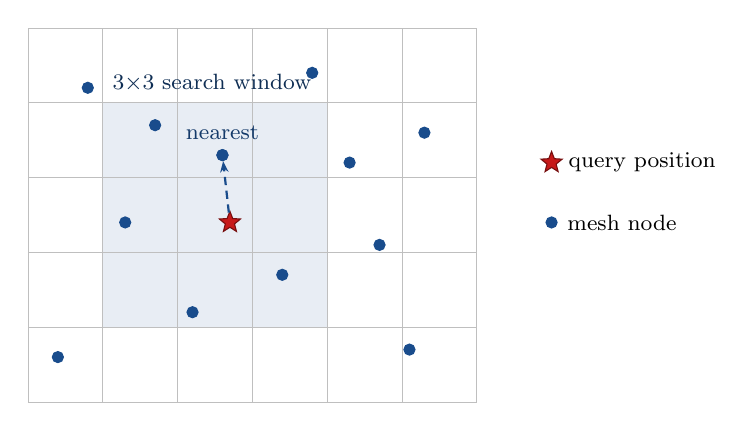
\begin{tikzpicture}[scale=0.95]
  \fill[lagblue!10] (1,1) rectangle (4,4);
  \draw[help lines,gray!50] (0,0) grid (6,5);
  \foreach \x/\y in {0.4/0.6,1.3/2.4,2.6/3.3,3.4/1.7,2.2/1.2,4.7/2.1,5.3/3.6,0.8/4.2,3.8/4.4,5.1/0.7,1.7/3.7,4.3/3.2}
     \node[meshnode] at (\x,\y) {};
  \node[drifter] (D) at (2.7,2.4) {};
  \node[meshnode,label={[nodelbl]above:nearest}] (NN) at (2.6,3.3) {};
  \draw[velarrow,densely dashed] (D)--(NN);
  \node[font=\footnotesize,lagblue!60!black,anchor=south west] at (1.0,4.02) {3$\times$3 search window};
  \node[drifter,label={[font=\footnotesize]right:query position}] at (7.0,3.2) {};
  \node[meshnode,label={[font=\footnotesize]right:mesh node}] at (7.0,2.4) {};
\end{tikzpicture}
\caption{Nearest-node search by spatial hashing. Nodes are bucketed into uniform cells when the mesh
is loaded. A query (the drifter) is first matched against the nodes of its own cell and the eight
neighbouring cells (shaded); \cref{sec:loc-exact} gives the test that decides whether this window is
enough.}
\label{fig:gridhash}
\end{figure}

\codeanchor{Construction \fn{build\_grid\_hash} (with \fn{\_gh\_lon\_branch},
\fn{\_gh\_grid\_geometry}, \fn{\_gh\_cell\_of}); node table \fn{\_node\_xyz\_fill} and its self-check
\fn{\_node\_xyz\_selfcheck}; window scan \fn{\_grid\_hash\_nearest\_3x3}; batch query
\fn{find\_nearest\_nodes}; all in \srcfile{core/mesh.py}.}

\section{Choosing the cell}\label{sec:loc-cell}

The reader of each mesh family proposes a cell of twice the mean node spacing,
\begin{equation}\label{eq:loc-legacy}
  c_{\text{legacy}}=\max\!\left(\ang{0.05},\;2\sqrt{A/N}\right),
\end{equation}
with $A$ the area of the mesh's longitude--latitude bounding box in square degrees. On a
quasi-uniform mesh this puts a few dozen nodes in the window at every resolution. On a mesh whose
resolution varies by orders of magnitude it does not: a cell sized for the coarse part holds
thousands of nodes where the mesh is fine, and the scan turns into a linear pass over them.

Every run therefore chooses the cell by measurement: the key
\conf{mesh.grid\_hash\_cell\_rule} defaults to \conf{occupancy}. The rule samples up to \num{200000} element centres, finds each one's exact
nearest node once, and evaluates the candidate cells $c_k=c_{\text{legacy}}/\sqrt{2}^{\,k}$,
$k=0,\dots,12$, without rebuilding the hash: for every sample it counts the nodes the window holds,
tests whether the window proves its answer (\cref{sec:loc-exact}), and estimates the cost of the query
--- the nodes scanned, the cells visited and one certificate per widening, a certificate weighing as
much as twenty cells. With the exact-anchor guard of \cref{sec:loc-exact} on (the default), the rule keeps
the reader's cell unless the cheapest eligible candidate (at most 20\,\% of the queries widened, at most
\SI{128}{MB} of offsets) is predicted to be at least 2.75 times cheaper; with the guard off it takes the
smallest cell that leaves no window empty, holds a median of at least eight nodes per window and has at
most half a percentage point more approximate anchors than the reader's cell. The ladder stops early where a candidate would need more than 64 rows of widening
budget or too many cells. With the guard on, quasi-uniform meshes keep the reader's cell and structure-resolving
meshes take a smaller one
(\cref{sec:perf-anchor}). An explicit \conf{mesh.grid\_hash\_cell\_size} overrides the rule, and
\conf{grid\_hash\_cell\_rule: legacy} keeps the reader's cell. The resolved cell and the rule are
written to the output metadata, so any run can be repeated with its cell pinned.

\codeanchor{\fn{choose\_grid\_hash\_cell} (the per-sample statistics in \fn{\_gh\_sample\_stats}),
\fn{apply\_grid\_hash\_cell\_rule}, \fn{set\_grid\_hash\_cell} and the one-line report
\fn{describe\_grid\_hash}, in \srcfile{core/mesh.py}; applied by \fn{run\_tracking} after the mesh is
loaded.}

\section{Exact nearest nodes}\label{sec:loc-exact}

A non-empty three-by-three window does not guarantee that the node it returns is the nearest one: a
closer node can lie just outside the window, most easily at high latitude, where a degree of longitude
shrinks, or with a cell smaller than the local node spacing. A near-nearest anchor changes the
interpolation stencil and, over time, the trajectory. With \conf{mesh.exact\_nearest: true} (the
default) the engine proves every anchor.

\paragraph{The certificate.} Let the window return a node at angular distance
$\theta=\arccos(\sin\phi_p\sin\phi_n+\cos\phi_p\cos\phi_n\cos\Delta\lambda)$ from the query. Any closer
node lies inside the spherical cap of radius $\theta$ around the query, whose half-extent is $\theta$
in latitude and
\begin{equation}\label{eq:loc-cap}
  \Delta\lambda_{\text{cap}}=\arcsin\!\left(\frac{\sin\theta}{\cos\phi_p}\right)
\end{equation}
in longitude, unbounded when $|\phi_p|+\theta\ge 90^\circ$ (the cap reaches a pole). The answer is
proven when the cap fits inside the latitude and longitude intervals the window actually searched ---
taking into account the narrower seam cell of a cyclic grid, a window clipped at the grid edge (there
are no nodes beyond it), and, on a non-cyclic grid, the $\pm360^\circ$ images of the cap
(\cref{fig:loc-certificate}). The test returns which sides fail: the rows, the columns, or --- when the
cap reaches a pole or an image of it meets the node range --- all columns.

\paragraph{Widening.} An unproven window grows in the failing direction --- rows and columns
independently, all columns only where required --- and is scanned again, new rows as contiguous slices,
until the best node found is proven. An empty window grows as a square until the first node is found,
or by whole rows in the polar cap, where a row's length $360^\circ\cos\phi$ is at most 32 cell widths. The growth has a budget: a query
whose nearest node is farther away than the longest element edge (plus two cells) lies outside every
element, so it keeps the best node seen and dies in that step; the budget, between 4 and 4096 rows, is
derived from the mesh when the hash is built.

\paragraph{One search for every path.} The batch query and every fused kernel's evaluation site call
the same exact search, so fused and unfused paths return the same anchor bit for bit, ties included,
and the fused kernels need no round trip through the batch path. With the guard off
(\conf{exact\_nearest: false}; together with \conf{grid\_hash\_cell\_rule: legacy} this reproduces the
nearest-node anchors of runs made before September 2026) the batch path keeps the plain window and
repairs empty windows through a $k$-d tree, and the fused kernels widen an empty window ring by ring ---
an approximate anchor. The two-dimensional barycentric kernels, and the least-squares kernels on HEALPix
pixel meshes, are then enabled only on meshes that pass a density certificate (every cell of every
element's bounding box has a non-empty window); the three-dimensional RK2 kernel instead flags a particle
whose window is empty and re-runs it with the anchor of the batch search (\cref{sec:fused-identity}).

\begin{figure}[t]
\centering
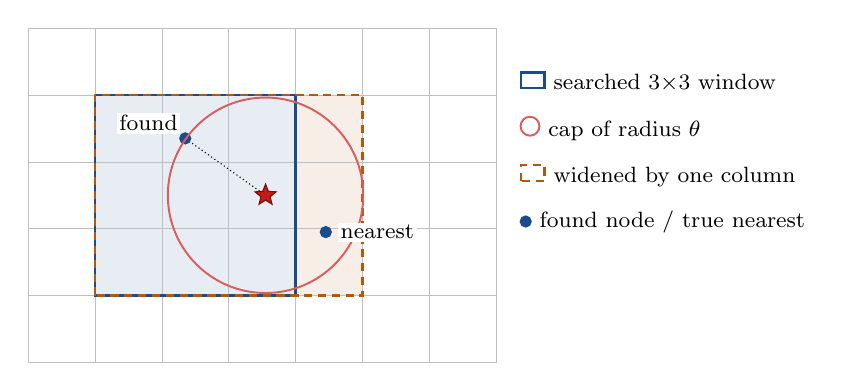
\begin{tikzpicture}[scale=0.85]
  \fill[lagblue!10] (1,1) rectangle (4,4);
  \fill[lagelem!10] (4,1) rectangle (5,4);
  \draw[help lines,gray!50] (0,0) grid (7,5);
  \draw[lagblue,line width=0.9pt] (1,1) rectangle (4,4);
  \draw[lagelem,line width=0.9pt,densely dashed] (1,1) rectangle (5,4);
  \node[drifter] (Q) at (3.55,2.5) {};
  \node[meshnode] (F) at (2.35,3.35) {};
  \draw[kelp!70,line width=0.7pt] (Q) ellipse (1.46 and 1.46);
  \draw[densely dotted] (Q)--(F);
  \node[meshnode] (T) at (4.45,1.95) {};
  \node[font=\footnotesize,anchor=west] at (7.2,4.2) {\tikz\draw[lagblue,line width=0.9pt](0,0)rectangle(0.3,0.2); searched 3$\times$3 window};
  \node[font=\footnotesize,anchor=west] at (7.2,3.5) {\tikz\draw[kelp!70,line width=0.7pt](0.15,0.1)circle(0.12); cap of radius $\theta$};
  \node[font=\footnotesize,anchor=west] at (7.2,2.8) {\tikz\draw[lagelem,line width=0.9pt,densely dashed](0,0)rectangle(0.3,0.2); widened by one column};
  \node[font=\footnotesize,anchor=west] at (7.2,2.1) {\tikz\node[meshnode]{}; found node / true nearest};
  \node[font=\footnotesize,fill=white,inner sep=1pt,above left=0pt and 0pt of F] {found};
  \node[font=\footnotesize,fill=white,inner sep=1pt,right=2pt of T] {nearest};
\end{tikzpicture}
\caption{The exactness certificate. The window returns a node at angular distance $\theta$; a closer
node can only lie in the cap of radius $\theta$ around the query. Here the cap crosses the window's
eastern edge, so the window cannot prove its answer; it widens by one column, finds the true nearest
node, and the smaller cap of the new answer fits inside the searched interval.}
\label{fig:loc-certificate}
\end{figure}

\codeanchor{Cap extents \fn{\_cap\_extents}; certificate \fn{\_anchor\_provable\_rect} (and
\fn{\_anchor\_provable} for the plain window); exact search \fn{\_grid\_hash\_nearest\_exact}; budget
\fn{\_gh\_far\_rows\_for}; guard flag \fn{set\_exact\_nearest}; guard-off single-particle search
\fn{\_grid\_hash\_nearest\_widened}; density certificate \fn{grid\_hash\_dense\_for\_elements}; all in
\srcfile{core/mesh.py}. The fused kernels anchor each site through \fn{\_fused\_site\_anchor} in
\srcfile{numerics/integrators.py}.}

\section{Where localization runs}\label{sec:loc-where}

Every evaluation site of the step re-queries the hash; no step path updates the anchor from the previous
one (only the offsets of the diffusivity gradient, \cref{ch:diffusion}, start a local walk from the
particle's node). A fused
kernel anchors its start, its stages and its final position through the exact search and tests the
final position for containment; the unfused paths query the batch search for the particles that
moved and test their containment. A particle folded back into a periodic window
(\cref{ch:lifecycle}) is re-anchored after the fold. On a HEALPix mesh in the geographic frame, points
poleward of the first ring of pixel centres lie outside every element and are lost; the rotated frame
of \cref{ch:frame} removes this limit.

\section{The containing element}\label{sec:loc-contain}

The nearest node does not by itself determine every interpolation stencil; several methods need the
element that \emph{contains} the particle. The engine scans the elements of the nearest node's
one-ring and tests each for containment (\cref{fig:contain}). If none contains the particle --- which
can occur on an irregular mesh, where the nearest node is not always a vertex of the containing
element --- the search widens to a second ring, scanning the elements adjacent to every vertex of the
one-ring elements. A particle for which neither ring yields a containing element is taken to lie
outside the domain; its step is undone and its status set to \code{OUTSIDE} (\cref{ch:lifecycle}).

\begin{figure}[t]
\centering
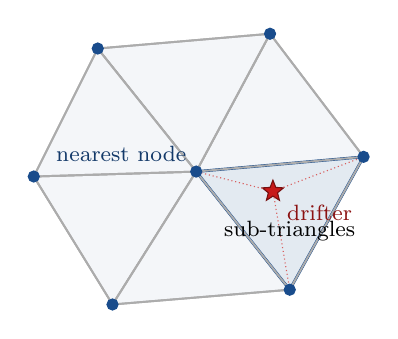
\begin{tikzpicture}[scale=1.25]
  \coordinate (C)  at (2.00,1.55);
  \coordinate (p1) at (0.35,1.50);
  \coordinate (p2) at (1.15,0.20);
  \coordinate (p3) at (2.95,0.35);
  \coordinate (p4) at (3.70,1.70);
  \coordinate (p5) at (2.75,2.95);
  \coordinate (p6) at (1.00,2.80);
  \foreach \a/\b in {p1/p2,p2/p3,p3/p4,p4/p5,p5/p6,p6/p1}
     \fill[meshface] (C)--(\a)--(\b)--cycle;
  \fill[hilface] (C)--(p3)--(p4)--cycle;
  \foreach \a/\b in {p1/p2,p2/p3,p3/p4,p4/p5,p5/p6,p6/p1}{
     \draw[meshedge] (C)--(\a); \draw[meshedge] (\a)--(\b);}
  \node[drifter] (D) at (2.78,1.35) {};
  \draw[densely dotted,kelp!70] (D)--(C);
  \draw[densely dotted,kelp!70] (D)--(p3);
  \draw[densely dotted,kelp!70] (D)--(p4);
  \foreach \p in {C,p1,p2,p3,p4,p5,p6} \node[meshnode] at (\p) {};
  \node[nodelbl,above left=0pt of C] {nearest node};
  \node[font=\footnotesize,kelp!70!black,below right=-1pt of D] {drifter};
  \node[font=\footnotesize] at (2.95,0.95) {sub-triangles};
\end{tikzpicture}
\caption{Containing-element search. The engine scans the one-ring of the nearest node and tests each
element for containment. The drifter lies in the shaded triangle; the dotted segments split it into
three sub-triangles whose signed areas, normalized by the whole, are the barycentric coordinates that
decide containment.}
\label{fig:contain}
\end{figure}

The containment test proceeds in three steps. First, the valid vertices of the candidate element are
compacted, discarding the $-1$ padding and, on the mixed meshes of FESOM-C, the repeated vertex.
Second, a dateline-safe bounding-box prefilter, in longitude differences wrapped to
$[-180^{\circ},180^{\circ})$, rejects candidates that cannot contain the point. Third, the element and
the point are projected to a local plane --- an equirectangular plane around the mean vertex,
$x=\Delta\lambda\,R\cos\phi_0$, $y=\Delta\phi\,R$, with the mean longitude taken on the wrapped
differences when the element straddles the dateline --- and the point is declared inside when its
barycentric coordinates are all non-negative to within a small negative tolerance, so that a point
exactly on an edge is inside and no particle falls between two neighbours. A near-degenerate triangle,
whose area falls below a second tolerance, is rejected rather than divided by. A quadrilateral is
tested on a fan of triangles, which is exact because quadrilaterals are required to be convex
(checked when the mesh is loaded, \cref{ch:mesh}); its interpolation weights are the Wachspress
coordinates of \cref{sec:hvel-quad}, computed separately.

\codeanchor{The ring search is \fn{\_find\_containing\_element\_local}; the containment test is
\fn{\_element\_contains} (bounding box) and \fn{\_polygon\_contains\_bool} (barycentric signs) on
\fn{\_project\_to\_local\_xy}; the tolerances \code{\_BARY\_EPS} $=-10^{-6}$ and \code{\_AREA\_TOL}
$=10^{-10}$ are module constants. All in \srcfile{core/mesh.py}.}

\section{Tracking the element across edges}\label{sec:loc-walk}

With \conf{numerics.elem\_search: walk} the containing element is searched once, when the run starts
(or taken from the checkpoint of a resumed run), and afterwards carried from step to step: at every evaluation site the engine starts from
the carried element and walks across edges towards the position. In an element with signed area $S$
and compacted vertices $(x_k,y_k)$, the edge coordinates of the point are
\begin{equation}\label{eq:loc-walk}
  w_k=\frac{\operatorname{sgn}S}{|S|}\,\bigl[(x_{k+1}-x_k)(p_y-y_k)-(p_x-x_k)(y_{k+1}-y_k)\bigr],
\end{equation}
and the point is inside when $\min_k w_k\ge-10^{-6}$; otherwise the walk crosses the edge with the
most negative $w_k$ into the neighbouring element. An acceptance within $10^{-2}$ of an edge is
re-checked with the exact containment predicate of \cref{sec:loc-contain}. Every outcome that is not a
clear containment --- a boundary edge, a two-element cycle, a degenerate element, or 256 steps --- falls
back to the ring search of \cref{sec:loc-contain}, so the walk returns the same element as the ring
search wherever that search is exhaustive and finds elements beyond the second ring where it is not.
The carried element is written to checkpoints. On a 28\,000-element mesh the walk costs
\SI{35}{ns} per particle against \SI{126}{ns} for the ring search; it runs on the unfused paths only
(the fused kernels keep their own search), which is why it pays off for element-layout barycentric
and edge least-squares interpolation and is left at \conf{local} on node-layout runs whose fused
kernels would otherwise be switched off.

\codeanchor{\fn{\_walk\_containing\_element} and \fn{find\_containing\_elements\_walk} in
\srcfile{core/mesh.py}; the element neighbours come from \fn{build\_elem\_neighbors}; the tracking
layer seeds and updates the carried elements (\fn{\_walk\_update\_elems} in
\srcfile{numerics/integrators.py}).}


\part{Interpolation in Space}
\chapter{Horizontal Velocity Interpolation}\label{ch:hvel}

Once a particle has been located (\cref{ch:localization}), the horizontal velocity must be
interpolated from the surrounding mesh values to the particle position. \textsf{KELP} provides
three schemes, selected by the configuration key \conf{uv\_interp}: a \emph{barycentric} scheme,
which blends the values at the vertices of the containing element; a \emph{least-squares} scheme
(the default), which fits a plane to the velocities at the element centres around the nearest node;
and an \emph{edge least-squares} scheme, which fits the plane to the containing element and its
edge neighbours, with a wall condition at the coast. The schemes are matched to the storage layout
of the velocity (\cref{sec:mesh-anatomy,tab:hvel-layouts}): the two least-squares schemes read
element-centre values, so supplying node-layout velocity to either is refused at startup. This
chapter gives the three schemes explicitly, including the local planar frames in which they compute,
and states the accuracy each achieves.

\begin{table}[t]
\centering\footnotesize\setlength{\tabcolsep}{4pt}
\begin{tabular}{@{}>{\raggedright\arraybackslash}p{58mm}>{\raggedright\arraybackslash}p{16mm}>{\raggedright\arraybackslash}p{50mm}@{}}
\toprule
velocity source & layout & admissible \conf{uv\_interp} \\
\midrule
FESOM2 \code{u}/\code{v}; FESOM-C element fields; HEALPix pixel geometry & element & \conf{leastsq}, \conf{edge\_leastsq}, \conf{barycentric} \\
FESOM2 \code{unod}/\code{vnod}; FESOM-C node fields; HEALPix dual mesh; NEMO (C-grid faces averaged to T-points) & node & \conf{barycentric} \\
\bottomrule
\end{tabular}
\caption{Velocity layouts by source and the interpolation schemes each admits. The layout is detected
from the field's dimensions; a metadata-only probe before the output file is created and a backstop
on the first step reject a mismatch with a message naming the fix.}
\label{tab:hvel-layouts}
\end{table}

\section{Projection to a local plane}\label{sec:hvel-projection}

All three schemes compute in a local planar frame rather than directly in longitude and latitude, so
that the spherical geometry is treated correctly away from the equator and across the dateline. The
two families use different frames.

\paragraph{Least-squares family.} The frame is centred on the particle $(\lonx_p,\latx_p)$ and scaled
by the metric at the particle's latitude,
\begin{equation}\label{eq:hvel-projection}
  z_0 = \cos\latx_p\cdot M, \qquad
  x_k = (\lonx_k-\lonx_p)\,z_0, \qquad
  y_k = (\latx_k-\latx_p)\,M ,
\end{equation}
with $M=\SI{111120}{\metre}$ per degree of latitude. The factor $\cos\latx_p$ is the essential
spherical correction: it shrinks the longitudinal axis so that a degree of longitude and a degree of
latitude map to their physical lengths. Across the dateline the plain least-squares scheme shifts an
element centre by one full turn only when the raw difference $\lonx_k-\lonx_p$ exceeds $\pm180^\circ$,
which leaves every stencil away from the seam bit-identical to the original arithmetic; the edge
least-squares scheme wraps every difference to $[-180^\circ,180^\circ)$.

\paragraph{Barycentric scheme.} The frame is centred on the element: its centre is the mean of the
vertices, with the longitudes accumulated as wrapped differences from the first vertex so that an
element straddling the dateline keeps its shape, and a point maps to
\begin{equation}\label{eq:hvel-projection-bary}
  x_k = \Delta\lonx_k \cdot \frac{\pi}{180}\, R \cos\latx_0, \qquad
  y_k = (\latx_k-\latx_0)\cdot \frac{\pi}{180}\, R ,
\end{equation}
where $(\lonx_0,\latx_0)$ is the frame centre, $\Delta\lonx_k$ the wrapped longitude difference and
$R$ the mesh's Earth radius. The weights computed below are ratios of areas in this plane and are
therefore independent of $R$; the radius serves only to keep the coordinates dimensionally
consistent.

\codeanchor{The projections are performed inline in \fn{\_interp\_leastsq\_core},
\fn{\_interp\_edge\_leastsq\_core} and \fn{\_interp\_barycentric\_core}
(\srcfile{numerics/interpolate.py}).}

\section{Barycentric interpolation}\label{sec:hvel-bary}

The barycentric scheme is the one scheme that serves node-layout velocity. The value at the particle
is the weighted average of the velocities at the vertices of the containing element, with weights
equal to the barycentric coordinates of the particle within it (\cref{fig:bary}); we give the
triangle here and the quadrilateral in \cref{sec:hvel-quad}. Let the projected triangle have vertices $1,2,3$ at
$(x_i,y_i)$ carrying velocities $(u_i,v_i)$, and let the particle project to
$(x_p,y_p)$. The barycentric coordinate $\bwt{i}$ is the area of the sub-triangle
\emph{opposite} vertex $i$ --- the sub-triangle formed by the particle and the other
two vertices --- divided by the area of the whole triangle:
\begin{equation}\label{eq:bary-area}
  \bwt{i} = \frac{\operatorname{area}(\text{sub-triangle opposite } i)}
                 {\operatorname{area}(\text{triangle})}, \qquad
  \bwt{1}+\bwt{2}+\bwt{3}=1 .
\end{equation}
A particle coinciding with vertex $i$ therefore has $\bwt{i}=1$ and the other weights
zero, and a particle on an edge has zero weight for the opposite vertex; the weights
vary continuously across element boundaries. In implemented form the weights are the
signed-area ratios
\begin{align}\label{eq:bary-explicit}
  D    &= (y_2-y_3)(x_1-x_3)+(x_3-x_2)(y_1-y_3), \notag\\
  \bwt{1} &= \frac{(y_2-y_3)(x_p-x_3)+(x_3-x_2)(y_p-y_3)}{D}, \\
  \bwt{2} &= \frac{(y_3-y_1)(x_p-x_3)+(x_1-x_3)(y_p-y_3)}{D}, \qquad
  \bwt{3} = 1-\bwt{1}-\bwt{2}, \notag
\end{align}
in which $D$ is twice the signed area of the triangle; a triangle whose $|D|$ falls
below a small tolerance is treated as degenerate and the interpolation reports
failure rather than dividing by it.

\begin{figure}[t]
\centering
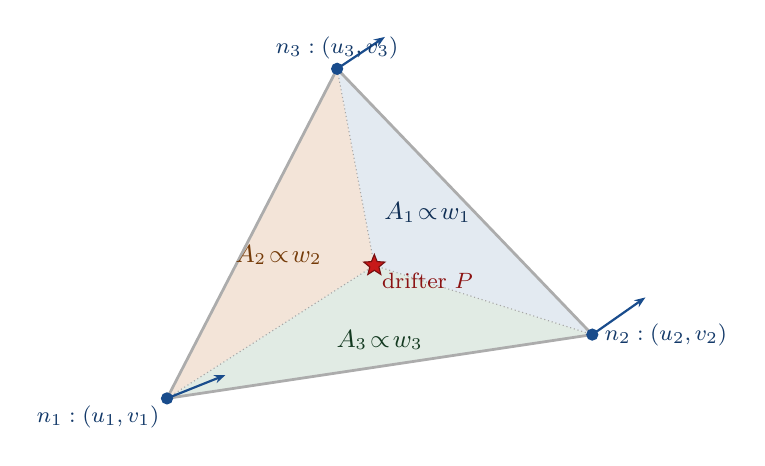
\begin{tikzpicture}[scale=1.35]
  \coordinate (N1) at (0.0,0.0);
  \coordinate (N2) at (4.0,0.6);
  \coordinate (N3) at (1.6,3.1);
  \coordinate (P)  at (1.95,1.25);
  % sub-triangles, one shade each
  \fill[lagblue!12]  (P)--(N2)--(N3)--cycle;   % opposite N1 -> w1
  \fill[lagelem!16]  (P)--(N3)--(N1)--cycle;   % opposite N2 -> w2
  \fill[laggreen!14] (P)--(N1)--(N2)--cycle;   % opposite N3 -> w3
  \draw[meshedge,line width=1pt] (N1)--(N2)--(N3)--cycle;
  \draw[densely dotted,gray!70] (P)--(N1) (P)--(N2) (P)--(N3);
  % sub-area labels
  \node[font=\small,lagblue!60!black]  at (2.45,1.75) {$A_1\!\propto\!\bwt{1}$};
  \node[font=\small,lagelem!65!black]  at (1.05,1.35) {$A_2\!\propto\!\bwt{2}$};
  \node[font=\small,laggreen!50!black] at (2.0,0.55)  {$A_3\!\propto\!\bwt{3}$};
  % velocity arrows at nodes
  \draw[velarrow] (N1)--++(0.55,0.22); \draw[velarrow] (N2)--++(0.5,0.35);
  \draw[velarrow] (N3)--++(0.45,0.3);
  % nodes & drifter
  \node[meshnode] at (N1) {}; \node[meshnode] at (N2) {}; \node[meshnode] at (N3) {};
  \node[drifter] at (P) {};
  \node[nodelbl,below left=-1pt of N1]  {$n_1:(u_1,v_1)$};
  \node[nodelbl,right=1pt of N2]        {$n_2:(u_2,v_2)$};
  \node[nodelbl,above=0pt of N3]        {$n_3:(u_3,v_3)$};
  \node[font=\footnotesize,kelp!70!black,below right=-1pt of P] {drifter $P$};
\end{tikzpicture}
\caption{Barycentric interpolation of node-layout velocity. The three triangle
vertices $n_1,n_2,n_3$ carry the node velocities $(u_i,v_i)$. The drifter $P$
splits the triangle into three sub-triangles; the weight $\bwt{i}$ is the area of
the sub-triangle \emph{opposite} vertex $i$ divided by the total area, so the
nearer the particle lies to a vertex, the larger that vertex's weight. The
interpolated velocity is $\bwt{1}(u_1,v_1)+\bwt{2}(u_2,v_2)+\bwt{3}(u_3,v_3)$.}
\label{fig:bary}
\end{figure}

The interpolated velocity is then the weighted sum of the three vertex velocities,
multiplied by the integration-direction factor of \cref{sec:arch-direction}:
\begin{equation}\label{eq:bary-blend}
  (U,V) = \tdir \sum_{i=1}^{3} \bwt{i}\,(u_i,v_i).
\end{equation}
For node-layout fields the vertex velocity $(u_i,v_i)$ is read directly from the
node. For element-layout fields handled through the same routine, each vertex value
is first formed as the area-weighted average of the velocities of the elements
sharing that vertex, $u_n=\sum_{e\ni n}A_e u_e\,/\sum_{e\ni n}A_e$ (a vertex whose areas sum to zero
fails the interpolation), and the blend \cref{eq:bary-blend} is applied to those vertex values. The scheme reproduces a
constant field exactly in both layouts and a linearly varying field exactly in the
node layout; in the element layout the vertex-averaging step makes it
smoothing rather than linearly exact. The interpolated field is continuous across element edges.
A quadrilateral element is handled by the same blend with Wachspress coordinates
\citep{warren1996barycentric,floater2003mvc} in place of the triangular weights of
\cref{eq:bary-area} (\cref{sec:hvel-quad}).

\codeanchor{The barycentric blend is \fn{\_interp\_barycentric\_core}
(\srcfile{numerics/interpolate.py}); the triangle weights
\cref{eq:bary-explicit} are \fn{\_barycentric\_weights\_tri} and the Wachspress
generalization \fn{\_wachspress\_weights\_quad} (\srcfile{core/mesh.py}).}

\section{Least-squares interpolation (element layout)}\label{sec:hvel-leastsq}

For element-layout velocity, the default scheme fits a plane to the velocities of
the element centres surrounding the nearest node and evaluates that plane at the
particle (\cref{fig:leastsq}). The stencil is the one-ring of elements about the
nearest node; their centres, carrying the element velocities $(u_e,v_e)$, are the
data. With the plane written $f(x,y)=a_0+a_1 x + a_2 y$ in the particle-centred
frame of \cref{eq:hvel-projection} (so the particle sits at the origin), the
coefficients minimize the residual
\begin{equation}\label{eq:leastsq}
  \min_{a_0,a_1,a_2}\ \sum_{e} \bigl(a_0 + a_1 x_e + a_2 y_e - f_e\bigr)^2 ,
\end{equation}
and because the frame is centred on the particle the interpolated value is simply
the constant term, $U=\tdir\,a_0^{(u)}$ and $V=\tdir\,a_0^{(v)}$. The minimization
reduces to a symmetric $3\times3$ system of normal equations, solved directly by
Cramer's rule. Centring the coordinates on the particle is not cosmetic: it avoids the
catastrophic cancellation that would arise from forming the normal equations with
raw longitude and latitude values. The system is declared singular, and the interpolation fails, when
\begin{equation}\label{eq:leastsq-guard}
  |\det A|<10^{-30}\quad\text{or}\quad |\det A|<10^{-12}\,|a_{11}a_{22}a_{33}| ,
\end{equation}
the second test being relative to the scale of the metric entries: a stencil of fewer than three
non-collinear centres --- a coastal node with only two elements, for instance --- has a determinant
of pure rounding noise, which an absolute test alone would pass. The same guard protects the
plane fits of the vertical velocity, the column height and the diffusivity; the scalar-sampling fit uses
an absolute threshold of $10^{-12}$ with the same relative test. The scheme is
exact for fields varying linearly over the stencil. Its stencil is the one-ring of the \emph{nearest
node}, so the interpolated field jumps where the nearest node changes, and the anchor must be exact
for two runs to agree (\cref{sec:loc-exact}).

\begin{figure}[t]
\centering
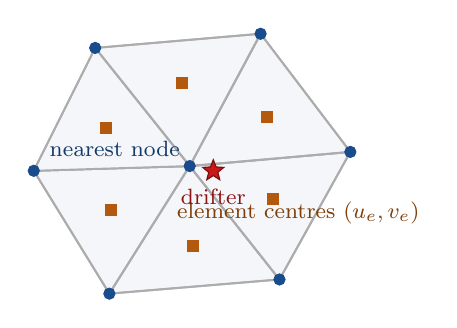
\begin{tikzpicture}[scale=1.2]
  \coordinate (C)  at (2.00,1.55);
  \coordinate (p1) at (0.35,1.50);
  \coordinate (p2) at (1.15,0.20);
  \coordinate (p3) at (2.95,0.35);
  \coordinate (p4) at (3.70,1.70);
  \coordinate (p5) at (2.75,2.95);
  \coordinate (p6) at (1.00,2.80);
  \foreach \a/\b in {p1/p2,p2/p3,p3/p4,p4/p5,p5/p6,p6/p1}{
     \fill[meshface] (C)--(\a)--(\b)--cycle;
     \draw[meshedge] (C)--(\a); \draw[meshedge] (\a)--(\b);}
  % element centres of the one-ring (the leastsq data)
  \foreach \a/\b in {p1/p2,p2/p3,p3/p4,p4/p5,p5/p6,p6/p1}
     \node[elemcentre] at ($ 0.3333*(C)+0.3333*(\a)+0.3333*(\b) $) {};
  \foreach \p in {C,p1,p2,p3,p4,p5,p6} \node[meshnode] at (\p) {};
  \node[drifter] (D) at (2.25,1.5) {};
  \node[nodelbl,above left=0pt of C] {nearest node};
  \node[elemlbl] at (3.15,1.05) {element centres $(u_e,v_e)$};
  \node[font=\footnotesize,kelp!70!black,below=1pt of D] {drifter};
\end{tikzpicture}
\caption{Least-squares interpolation of element-layout velocity. The data are the
velocities at the centres (orange squares) of the one-ring of elements about the
nearest node. A plane $f=a_0+a_1x+a_2y$ is fitted to them in a frame centred on the
drifter, so the interpolated velocity is the fitted constant $a_0$. The scheme is
exact for linearly varying fields over this stencil.}
\label{fig:leastsq}
\end{figure}

The schemes are tied to the storage layout, and the engine enforces the match rather than silently
producing a wrong answer. Because both least-squares schemes index velocities at element centres,
supplying them with node-layout velocities such as \conf{unod}/\conf{vnod} is a category error; the
engine detects the mismatch from the field's dimensions and raises a configuration error at startup,
with the message that node-based velocities require \conf{uv\_interp}${}={}$\conf{barycentric}. The
check is performed both during a metadata-only probe before any data is read and as a backstop on the
first step, so the run fails fast and informatively rather than midway through.

\codeanchor{The plane fit is \fn{\_interp\_leastsq\_core}
(\srcfile{numerics/interpolate.py}); the layout-compatibility check that rejects
node velocities under both least-squares schemes is \fn{\_validate\_uv\_compat}
(\srcfile{tracking.py}), fed by each reader's \fn{probe\_uv\_layout}.}

\section{Edge least-squares interpolation}\label{sec:hvel-edge}

The edge least-squares scheme (\conf{uv\_interp: edge\_leastsq}) fits the same plane as
\cref{eq:leastsq}, in the particle-centred frame, but over a different stencil: the centre of the
element that contains the particle and the centres of the elements across each of its edges --- four
points for a triangle, five for a quadrilateral (\cref{fig:edge-lsq}). The stencil follows the
containing element rather than the nearest node, as in the finite-volume discretisation of the FESOM
models, and it needs the containing element, so a particle outside every element fails the
interpolation. The plane is exact for a linear field in the interior.

At the coast an edge has no neighbour. It contributes a \emph{ghost} point instead: the own centre
$\mathbf{c}$ mirrored across the edge, $\mathbf{g}=2\mathbf{f}-\mathbf{c}$, with $\mathbf{f}$ the foot of
$\mathbf{c}$ on the edge. With $\hat{\mathbf{t}}$ the unit tangent of the edge and $\mathbf{u}$ the own
velocity, the ghost carries
\begin{equation}\label{eq:edge-ghost}
  \mathbf{u}_g =
  \begin{cases}
    2(\mathbf{u}\cdot\hat{\mathbf{t}})\,\hat{\mathbf{t}}-\mathbf{u} & \text{free slip (default)},\\
    -\mathbf{u} & \text{no slip},
  \end{cases}
\end{equation}
selected by \conf{edge\_leastsq\_bc}. The free-slip ghost is the mirror image of the own velocity ---
its tangential component kept and its normal component reversed --- so the fitted plane carries a
flow parallel to the wall exactly and damps the flow through it. The no-slip ghost makes the plane
vanish near the wall; being a single plane fitted to both sides, it overshoots on the interior side of
a wall element and can reverse the flow near a corner between two walls, a property of the fit rather
than a defect. A boundary edge of zero length contributes no point. The stencil stays well conditioned
even on very thin elements, because the mirrored ghosts span both directions.

\begin{figure}[t]
\centering
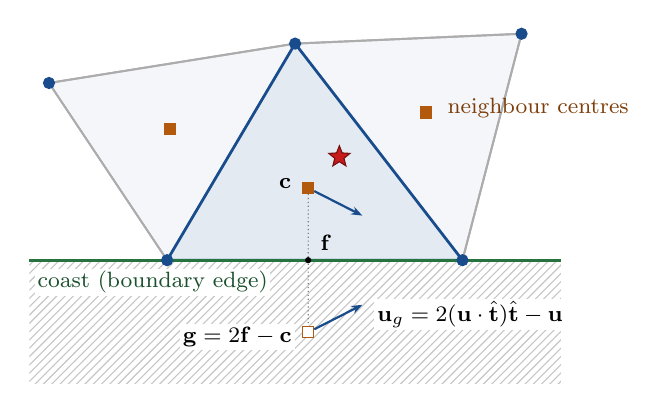
\begin{tikzpicture}[scale=1.25]
  \coordinate (A) at (0,0); \coordinate (B) at (3,0); \coordinate (C) at (1.3,2.2);
  \coordinate (D) at (3.6,2.3); \coordinate (E) at (-1.2,1.8);
  \fill[pattern=north east lines,pattern color=gray!45] (-1.4,0)--(4.0,0)--(4.0,-1.25)--(-1.4,-1.25)--cycle;
  \fill[meshface] (B)--(C)--(D)--cycle; \fill[meshface] (C)--(A)--(E)--cycle;
  \fill[hilface] (A)--(B)--(C)--cycle;
  \draw[meshedge] (B)--(D)--(C) (C)--(E)--(A);
  \draw[laggreen,line width=1.2pt] (-1.4,0)--(4.0,0);
  \node[font=\footnotesize,laggreen!70!black,fill=white,inner sep=1pt,anchor=north west] at (-1.35,-0.08) {coast (boundary edge)};
  \foreach \p in {A,B,C,D,E} \node[meshnode] at (\p) {};
  \node[elemcentre] (c) at (1.433,0.733) {};
  \node[elemcentre] at (2.633,1.5) {};
  \node[elemcentre] at (0.033,1.333) {};
  \node[elemcentre,fill=white] (g) at (1.433,-0.733) {};
  \draw[densely dotted,gray] (c)--(g);
  \node[circle,fill=black,inner sep=0.8pt] at (1.433,0) {};
  \node[font=\footnotesize,anchor=south west] at (1.46,0.0) {$\mathbf{f}$};
  \draw[velarrow] (c)--++(0.55,-0.28);
  \draw[velarrow] (g)--++(0.55,0.28);
  \node[font=\footnotesize,anchor=east] at (1.36,0.78) {$\mathbf{c}$};
  \node[font=\footnotesize,fill=white,inner sep=1pt,anchor=east] at (1.3,-0.78) {$\mathbf{g}=2\mathbf{f}-\mathbf{c}$};
  \node[drifter] at (1.75,1.05) {};
  \node[font=\footnotesize,fill=white,inner sep=1pt,anchor=west] at (2.1,-0.55) {$\mathbf{u}_g=2(\mathbf{u}\cdot\hat{\mathbf{t}})\hat{\mathbf{t}}-\mathbf{u}$};
  \node[elemlbl,anchor=west] at (2.75,1.55) {neighbour centres};
\end{tikzpicture}
\caption{The edge least-squares stencil. The drifter lies in the shaded triangle; the plane is fitted
to its centre $\mathbf{c}$ and the centres of the elements across its two interior edges. Its third
edge is on the coast and contributes a ghost at the mirror image $\mathbf{g}$ of $\mathbf{c}$, carrying
the mirrored velocity: the component along the wall is kept and the component into the wall reversed
(free slip), or the whole velocity reversed (no slip).}
\label{fig:edge-lsq}
\end{figure}

\codeanchor{\fn{\_interp\_edge\_leastsq\_core} (\srcfile{numerics/interpolate.py}); the edge
neighbours are \fn{build\_elem\_neighbors} (\srcfile{core/mesh.py}), built once when the run
starts.}

\section{Interpolation on mixed meshes: quadrilateral elements}\label{sec:hvel-quad}

The barycentric scheme of \cref{sec:hvel-bary} generalizes from the triangular meshes of FESOM2 to
meshes with quadrilaterals: the mixed meshes of FESOM-C, the dual mesh built from a HEALPix grid
(mostly quadrilaterals; an all-wet sphere has exactly eight triangles), the pixel geometry of a
HEALPix grid and the meshes built from structured NEMO grids (quadrilaterals only). Every horizontal
interpolator is split into a \emph{geometric weight stage}, which depends on the number of vertices of
the containing element, and a \emph{value stage}, which depends only on the field layout. The plain
least-squares scheme bypasses the geometric stage entirely --- it reads one velocity per element
centre --- and is identical on triangles and quadrilaterals; the edge least-squares scheme differs only
in the number of edges.

Before the weight stage, the element's vertices are compacted: the $-1$ padding is removed, and a
triangle that FESOM-C has stored as a quadrilateral with a repeated leading vertex is reduced to its
three distinct vertices. A triangle on a mixed mesh is therefore interpolated by the triangular
weights of \cref{eq:bary-explicit}, bit-for-bit as on a pure FESOM2 mesh; only a genuine four-vertex
element takes the quadrilateral path.

For a quadrilateral the weights are the Wachspress generalized barycentric coordinates
\citep{warren1996barycentric,floater2003mvc}, the natural analogue of \cref{eq:bary-area} for a convex
polygon (\cref{fig:wachspress}). With the four vertices $u_1,\dots,u_4$ in cyclic order, the particle
$p$, and the doubled signed areas
\begin{equation}\label{eq:wachspress}
  A_k = 2\operatorname{area}(p,u_k,u_{k+1}), \qquad
  C_k = 2\operatorname{area}(u_{k-1},u_k,u_{k+1}),
\end{equation}
the classical weight is $C_k/(A_{k-1}A_k)$, normalized over the vertices. The engine uses its
\emph{product form}, the classical weight multiplied by $A_1A_2A_3A_4$,
\begin{equation}\label{eq:wachspress-product}
  \bwt{k} = \frac{C_k\,A_{k+1}\,A_{k+2}}{\sum_{j} C_j\,A_{j+1}\,A_{j+2}} ,
\end{equation}
which contains no division by an area that vanishes on an edge: on an edge it reduces exactly to
linear interpolation along that edge and at a vertex to that vertex's indicator. Each term carries
three signed areas, so a clockwise element negates every term and the normalization cancels it; no
orientation handling is needed. The coordinates reproduce a linear field exactly, are smooth in the
interior and give every vertex a non-zero weight.

\begin{figure}[t]
\centering
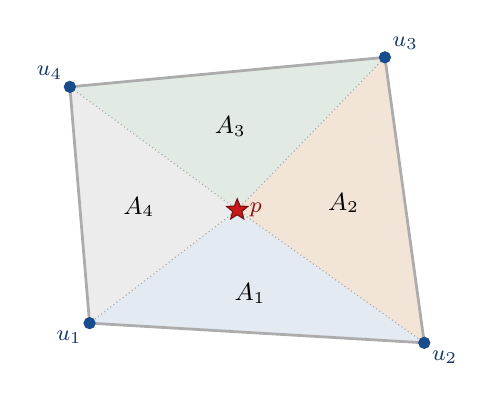
\begin{tikzpicture}[scale=1.25]
  \coordinate (v1) at (0.2,0.2);
  \coordinate (v2) at (3.6,0.0);
  \coordinate (v3) at (3.2,2.9);
  \coordinate (v4) at (0.0,2.6);
  \coordinate (P)  at (1.70,1.35);
  \fill[lagblue!12]  (P)--(v1)--(v2)--cycle;
  \fill[lagelem!16]  (P)--(v2)--(v3)--cycle;
  \fill[laggreen!14] (P)--(v3)--(v4)--cycle;
  \fill[gray!15]     (P)--(v4)--(v1)--cycle;
  \draw[meshedge,line width=1pt] (v1)--(v2)--(v3)--(v4)--cycle;
  \draw[densely dotted,gray!70] (P)--(v1) (P)--(v2) (P)--(v3) (P)--(v4);
  \node[font=\small] at (1.83,0.50) {$A_1$};
  \node[font=\small] at (2.78,1.42) {$A_2$};
  \node[font=\small] at (1.63,2.20) {$A_3$};
  \node[font=\small] at (0.70,1.38) {$A_4$};
  \node[meshnode] at (v1) {}; \node[meshnode] at (v2) {};
  \node[meshnode] at (v3) {}; \node[meshnode] at (v4) {};
  \node[drifter] at (P) {};
  \node[nodelbl,below left=-1pt of v1]  {$u_1$};
  \node[nodelbl,below right=-1pt of v2] {$u_2$};
  \node[nodelbl,above right=-1pt of v3] {$u_3$};
  \node[nodelbl,above left=-1pt of v4]  {$u_4$};
  \node[font=\footnotesize,kelp!70!black,right=1pt of P] {$p$};
\end{tikzpicture}
\caption{Wachspress interpolation on a quadrilateral element. The drifter $p$ splits the element into
four fan triangles of doubled area $A_1,\dots,A_4$. The weight at vertex $k$ is proportional to
$C_k A_{k+1} A_{k+2}$, where $C_k$ is the doubled area of the corner triangle $(u_{k-1},u_k,u_{k+1})$:
the two fan triangles \emph{not} adjacent to vertex $k$ grow as $p$ approaches it.}
\label{fig:wachspress}
\end{figure}

The formula needs no guard and has no fall-back because quadrilaterals are required to be convex:
the FESOM-C reader, the builder of structured-grid meshes and the HEALPix builders check every
quadrilateral when the mesh is loaded and name the offending elements if one is not convex.

The \emph{containment} test of \cref{sec:loc-contain}, which decides whether a particle lies inside a
quadrilateral, uses a fan of triangles --- never the Wachspress construction, which enters only the
weight stage after containment has been established. The same vertex-count branch governs the
\conf{barycentric} option of the vertical-velocity combine (\cref{sec:vert-whoriz}) and of scalar
sampling (\cref{ch:sampling}); the \conf{nearest}, \conf{idw} and \conf{leastsq} options of those
routines are independent of element shape. Element areas enter only when an element-layout vertex
value is formed as an area-weighted average (\cref{sec:hvel-bary}). They are read from the model's mesh
file when it provides them (FESOM2 mesh diagnostics do; ASCII meshes and regional extracts do not); otherwise they are computed on the sphere as the
spherical excess of the element's fan of triangles times the square of the mesh radius. Because they
appear only as ratios, their absolute scale is immaterial.

\section{Common properties}\label{sec:hvel-common}

\paragraph{Three dimensions.} In a three-dimensional run the horizontal velocity is piecewise constant
in the vertical: each particle reads the layer found in \cref{sec:vert-layer}, and the scheme is applied
to that layer's field without vertical interpolation.

\paragraph{Time.} Between two snapshots the time-aware variants blend the two fields in time for each
element or vertex they read, before the unchanged spatial formula (\cref{ch:temporal,ch:fused}).

\paragraph{Failure.} A scheme that cannot interpolate --- a singular fit, no containing element, a
degenerate triangle --- reports failure; the particle's step is undone, its status set to
\code{OUTSIDE} and its failure reason to an interpolation failure (\cref{ch:lifecycle}).

\paragraph{Element tracking.} With \conf{elem\_search: walk} (\cref{sec:loc-walk}) the barycentric and
edge least-squares schemes receive the containing element from the walk and skip their own search; the
plain least-squares scheme does not use it.

\codeanchor{The weight dispatcher is \fn{\_polygon\_weights}; the triangular and Wachspress weights are
\fn{\_barycentric\_weights\_tri} and \fn{\_wachspress\_weights\_quad}; the convexity check is
\fn{validate\_quad\_convexity} with \fn{find\_nonconvex\_quads}; element areas are
\fn{build\_elem\_areas}; all in \srcfile{core/mesh.py}. The vertex compaction is in
\fn{\_interp\_barycentric\_core} (\srcfile{numerics/interpolate.py}).}

\codenote{The projections use three radii: the barycentric horizontal-velocity kernel uses the mesh
radius, the containment test and the vertical-velocity and scalar barycentric kernels use
\SI{6371000}{\metre}, and the least-squares family uses \SI{111120}{\metre} per degree. The weights
are ratios of areas in the projected plane and the least-squares value is the fitted constant, so the
interpolated values do not depend on the radius; we record the difference only for fidelity to the
source.}

\chapter{Vertical Structure and Vertical-Velocity Interpolation}\label{ch:vertical}

In a three-dimensional run the particle also moves vertically, driven by the model vertical velocity
$\Wvel$. This chapter describes the sign convention of $\Wvel$ and how each reader establishes it,
how the depth coordinate is organized for the two vertical-coordinate families, how the layer
containing a particle is found, how the horizontal velocity is read in depth --- per layer or linearly
between its data points --- how $\Wvel$ is interpolated to the particle in the vertical and then
in the horizontal, how a step advances the depth on a terrain-following mesh, and how a particle is
held within the water column. The two families are the fixed depth levels (z-levels) of FESOM2, FESOM~1.4
and the HEALPix products, and the terrain-following sigma coordinate of FESOM-C; they are implemented by
\emph{separate} routines throughout, and we give each explicitly. Depth $\depx$ and vertical velocity
$\Wvel$ are positive downward (\cref{sec:intro-conv}). On a z-level mesh the vertical position update
is
\begin{equation}\label{eq:vert-update}
  \depx_{n+1} = \depx_n + \Wvel\,\dt ,
\end{equation}
which deepens a particle wherever the flow is downwelling; on a sigma mesh the step advances the
particle's fraction of the water column instead (\cref{sec:vert-sigma-step}).

\section{The sign of the vertical velocity}\label{sec:vert-wsign}

Inside the engine the vertical velocity is the positive-down rate of the tracked depth. Ocean models
write the opposite sign, and every reader converts once, when a snapshot is read
(\cref{tab:vert-wsign}). The convention of a file is resolved in this order: the configuration key
\conf{mode.w\_positive} when it is \conf{up} or \conf{down}; otherwise the variable's CF
\code{positive} attribute; otherwise a CF \code{standard\_name} beginning with \code{upward} or
\code{downward}; otherwise the default of the reader's producer. The default, \conf{auto}, therefore
needs no setting for model output. For a FESOM2 dataset without a vertical velocity, the tool
\code{utils/reconstruct\_w.py} reconstructs one offline from $u$, $v$ and the sea-surface height, by
integrating the horizontal divergence down the column; it writes the result positive down, with the
attribute that says so.

\begin{table}[t]
\centering\footnotesize\setlength{\tabcolsep}{4pt}
\begin{tabular}{@{}p{30mm}p{20mm}p{62mm}p{16mm}@{}}
\toprule
producer (reader) & variable & file convention & conversion \\
\midrule
FESOM2 (\code{fesom2}) & \code{w} & positive up; in the zstar coordinate the velocity \emph{through} the moving interfaces & negated \\
HEALPix products (\code{healpix}) & \code{wo}, \code{avg\_wo} & positive up (``upward sea water velocity'') & negated \\
FESOM-C (\code{fesomc}) & \code{w} & positive up; the flux through the sigma interfaces per unit area, zero at the surface and the bottom & negated \\
offline reconstruction & \code{w} & positive down, attribute \code{positive = "down"} & none \\
\bottomrule
\end{tabular}
\caption{Vertical-velocity conventions of the supported producers and the conversion each reader
applies. The FESOM-C diagnostic \code{w\_cart} is refused: its flux term lacks the dia-sigma part of the
Cartesian vertical velocity.}
\label{tab:vert-wsign}
\end{table}

\codenote{Engine versions before September 2026 applied no conversion, so their three-dimensional
FESOM2 and HEALPix runs moved particles vertically in the wrong direction. The sign is now tested
against the equatorial upwelling in real model output. A vertical-velocity file written by the offline
reconstruction before that date carries no attribute and is read with \conf{w\_positive: down}.}

\paragraph{The zstar coordinate of FESOM2.} FESOM2's interfaces move with the sea surface, and its
\code{w} is the flow through them. The engine integrates it on the fixed reference levels, where the
horizontal velocities also live, which drops the factor $H/(H+\eta)$ of the zstar equation: a relative
error $\eta/H$ in the vertical rate, about $10^{-4}$ in the deep ocean and \SIrange{1}{2}{\percent} on a
shelf \SIrange{50}{100}{\metre} deep. The recorded depth is the zstar (reference) depth, which differs
from the physical depth by $\eta\,(1-\depx/H)$, at most $|\eta|$.

\codeanchor{\fn{resolve\_w\_sign} in \srcfile{readers/\_\_init\_\_.py}, applied by the FESOM2,
HEALPix and FESOM-C readers; the key \conf{mode.w\_positive} is validated in \srcfile{core/config.py}.}

\section{Vertical coordinate: z-levels and sigma}\label{sec:vert-coord}

The two families are distinguished only by how an interface depth is obtained, but the difference
propagates through every routine below. For the \emph{z-level} family the interface depths are a
fixed array $z_0=0<z_1<\dots<z_{K-1}$, the same at every horizontal location; the per-node sea floor is
the separate array \code{depth}. FESOM2 meshes hold the levels in the mesh file. FESOM~1.4 meshes take
them from \code{nod3d.out} or from the depth coordinate of level-wise data, and their per-node floor is
the depth of each column's last wet level (\cref{sec:mesh-fesom14}). A HEALPix product
takes them from \conf{mesh.levels} --- the path of a level table or an inline list of depths, required to
be strictly increasing --- or from the table a regional extract embeds; its per-node floor comes from
a bathymetry variable when the store has one, otherwise from the deepest level with finite data. For
the terrain-following \emph{sigma} family of FESOM-C the interface depths are reconstructed per water
column from a fixed set of fractions $\sigma_k$ and the local column thickness $H$,
\begin{equation}\label{eq:sigma}
  H = \max(d+\eta,\,D_{\min}), \qquad z_k = (1-\sigma_k)\,H,
\end{equation}
where $d$ is the still-water depth, $\eta$ the sea-surface height, and $D_{\min}$ a configurable minimum
thickness (default \SI{0.5}{\metre}). With this convention $\sigma=1$ maps to $z=0$ (the surface) and
$\sigma=0$ maps to $z=H$ (the floor). The key \conf{mode.max\_levels} keeps the top
\conf{max\_levels} interfaces of either family.

\codenote{The FESOM2 NetCDF and Zarr loaders store the z-levels positive down; the
\code{mesh.z\_levels} property takes the absolute value once more. Three-dimensional runs on FESOM2's
legacy ASCII mesh format are unsupported: its level reader takes the whole \code{aux3d.out} file, node depths
included, as the level table. (The FESOM~1.4 reader reads its own, different \code{aux3d.out} format
correctly, \cref{sec:mesh-fesom14}.) For sigma meshes the orientation $\sigma=1$ (surface) to $\sigma=0$ (floor) is
assumed by \cref{eq:sigma} but is \emph{not} validated when the mesh is read: a file written with the
opposite ordering would silently invert the column.}

On z-level meshes $\eta$ does not enter the vertical path at all: the layer search, the
vertical-velocity profile and the depth clamp depend only on the fixed levels and the per-node floor.
On sigma meshes $\eta$ sets the column thickness everywhere, and the column that matters is the one
\emph{at the particle}: every routine below uses $H_p$, the column thickness interpolated to the
particle position by the same horizontal method as the vertical velocity (\cref{sec:vert-whoriz}).

\section{Finding the layer}\label{sec:vert-layer}

Given a particle depth $\depx$, the engine identifies the layer that contains it, and the two families
do this differently. On a z-level mesh the search is over the fixed interfaces: a particle at or above
$z_0$ is assigned to the top layer, and otherwise the layer is the index $k$ with
$z_k\le\depx<z_{k+1}$. The search is bounded below by the local floor through a specific rule --- the
deepest admissible layer is $\max(k^\ast-1,0)$, where $k^\ast$ is the first index whose lower interface
$z_{k+1}$ exceeds the per-node bottom depth --- so a particle is never placed in a layer that lies below
its local sea floor. On a sigma mesh the search is over the interfaces $z_k=(1-\sigma_k)H_p$ of the
particle's own column; its deepest layer is simply $K-2$, bounded by the bottom interface, with no
analogue of the z-level step-back. This asymmetry is a genuine difference in behaviour between the two
families at the deepest layer, not merely a difference in formulae.

\codeanchor{Layer location is \fn{find\_layer}/\fn{find\_layers} (\srcfile{numerics/vertical.py},
z-level) and \fn{find\_layer\_sigma}/\fn{find\_layers\_sigma} (\srcfile{numerics/vertical\_sigma.py},
sigma, with the particle column passed as \code{H\_particle}); the per-particle layer index is
assembled by \fn{\_compute\_layers} (\srcfile{numerics/integrators.py}).}

\section{Horizontal velocity in depth: layers or linear}\label{sec:vert-uvdepth}

The horizontal velocity of a three-dimensional run is stored at a few discrete depths per column,
and the engine offers two rules for reading it in between, selected by \conf{mode.uv\_vertical}.
Most producers write $u$ and $v$ once per layer, at the layer centre: the FESOM2 node fields
\code{unod}/\code{vnod} and element fields \code{u}/\code{v}, the HEALPix \code{uo}/\code{vo}, and the
FESOM-C \code{u}/\code{v} on its sigma layers, $K-1$ rows each. Under the default, \conf{layer}, the
velocity is \emph{piecewise constant in depth}: every member of the horizontal stencil of \cref{ch:hvel}
--- a vertex or an element --- reads the row of the particle's layer, found by the rule of
\cref{sec:vert-layer} in the nearest node's column (on a sigma mesh, in the particle's own column), so a
particle that crosses a level sees the velocity jump. Under \conf{linear} the same data are read
\emph{linearly in depth} between the layer centres, and every member is read in its own column. FESOM~1.4
writes $u$ and $v$ on the levels themselves, and its fields are always read linearly in depth. Inside the
engine the rule is a property of the field, its \emph{placement} \code{VelocityField.uv\_vertical}, with the
three values of \cref{tab:vert-uv-placement}. This section gives the rule, the treatment of a stencil
member whose sea floor lies above the particle, its form on sigma meshes and for FESOM~1.4, and the
combinations the engine refuses.

\begin{table}[t]
\centering\footnotesize\setlength{\tabcolsep}{4pt}
\begin{tabular}{@{}>{\raggedright\arraybackslash}p{27mm}>{\raggedright\arraybackslash}p{24mm}>{\raggedright\arraybackslash}p{46mm}>{\raggedright\arraybackslash}p{40mm}@{}}
\toprule
placement & rows of $u$, $v$ & data points $p_k$ (positive down) & set by \\
\midrule
\code{"layer"} & $K-1$ & none: one value per layer & every reader; the default \\
\code{"layer\_linear"} & $K-1$, node or element layout & the layer centres $\tfrac12(z_k+z_{k+1})$; on a sigma mesh $1-\tfrac12(\sigma_k+\sigma_{k+1})$, in the sigma fraction & \conf{mode.uv\_vertical: linear}; the tracking layer marks every field it reads \\
\code{"level"} & $K$, node layout & the levels $z_k$ & the FESOM~1.4 reader; the option is refused there \\
\bottomrule
\end{tabular}
\caption{The three placements of the horizontal velocity in depth. Only \code{"layer"} is piecewise
constant; the other two are read by the depth-linear rule of this section.}
\label{tab:vert-uv-placement}
\end{table}

\paragraph{The data-point table.} For a depth-linear field the engine builds, once per mesh, placement
and layout, a table of the data points $p_0\le p_1\le\dots\le p_{M-1}$ ($M=K$ for levels, $M=K-1$ for
layer centres) and, for every \emph{column} $c$ --- a node for node-layout fields, an element for
element-layout fields --- two numbers: the index $\ell_c$ of its \emph{last usable point}, the deepest
point it may be read at, and its \emph{bed} $d_c$, the physical depth of its sea floor. For a node $i$,
\begin{equation}\label{eq:vert-uv-last}
  \ell_i = \max\Bigl(0,\ \min\bigl(M-1,\ \max(\{k : l_k\le d_i\}\cup\{0\}),\ D_i\bigr)\Bigr),
\end{equation}
where $l_k=p_k$ for level data and $l_k=z_{k+1}$, the layer's \emph{lower} level, for layer data;
$d_i$ is the node's bed \code{mesh.depth}, and $D_i$ an optional declaration by the reader of the last
finite point of its own data column (\code{mesh.metadata["uv\_data\_last"]}). For layer data this is the
rule of the layer search (\cref{sec:vert-layer}): a \emph{partial bottom layer}, one whose lower level lies
below the bed, is never read. The HEALPix reader declares where each column's $u$ data end, and the
FESOM~1.4 reader declares each column's last wet level; $D_i=-1$ means ``the surface only'', and the
surface value must then be finite. A NaN bed matches no level, which gives $\ell_i=0$; an infinite bed
follows the formula as written ($+\infty$ keeps every point, $-\infty$ the surface point only). For an
element $e$ the node depths cannot tell where its water ends --- FESOM2 fixes the number of levels of each
element first and gives a node the deepest of its elements --- so the element table takes both numbers
from the reader: $\ell_e=\max(0,\min(M-1,D_e))$ with $D_e$ the element's last wet layer
(\code{uv\_data\_last\_elem}), and $d_e$ its bed (\code{elem\_bed}), which the FESOM2 reader derives from
the mesh diagnostic (\cref{sec:mesh-elem-bottoms}). A \conf{mode.max\_levels} cut caps every $\ell_c$ at
the last kept point and leaves the bed unchanged. Points below $\ell_c$ are \emph{never read}, not even
multiplied by zero, so dry or fill values stored there are harmless.

\codeanchor{The table is \fn{depth\_points} with the frozen dataclass \fn{DepthPoints} (fields \code{p},
\code{last}, \code{bed}) and the builder \fn{\_build\_depth\_points}, in \srcfile{numerics/vertical\_uv.py}.
It is cached on the mesh per placement and layout and rebuilt whenever \code{mesh.sigma}, the bed array or
the declaration is replaced; the engine builds it from its own read-only snapshot of the declaration
(\fn{\_snapshot\_declaration}), which replaces the reader's array in \code{mesh.metadata}.}

\paragraph{Bracket and blend.} At a column $c$ and particle depth $z$ the depth is first clipped into the
column's usable range, the bracketing points $p_k\le z_c<p_{k+1}$ (with $k+1\le\ell_c$) are found, and
the stored values $f$ ($u$ or $v$) are blended:
\begin{equation}\label{eq:vert-uv-blend}
  z_c = \max\bigl(p_0,\ \min(z,\ p_{\ell_c})\bigr),\qquad
  f_c(z) = (1-\interpfrac)\,f_{k,c} + \interpfrac\,f_{k+1,c},\qquad
  \interpfrac = \frac{z_c-p_k}{p_{k+1}-p_k}.
\end{equation}
Above the first point and below the last usable point the value of that point is used: the ends are
constant, and nothing is extrapolated. A depth exactly on a point, at either end, or in a degenerate
interval (a spacing below $10^{-12}$) reads the point directly, without touching its neighbour; of two
coincident points the deeper one is read, except at the surface end, where a depth at or above $p_0$
reads point~0. Single-precision data are widened to double precision before the blend. Because the
bracket depends only on the column's own $\ell_c$, a member whose last usable point lies above the
particle --- a partial bottom layer, a \conf{max\_levels} cut, a declared prefix that ends above the bed ---
contributes the value of that point, provided it holds water at $z$ (\cref{fig:vert-uv}).

\codeanchor{\fn{uv\_bracket} returns $(k,\interpfrac)$, with $\interpfrac<0$ meaning ``read point $k$
directly'', and \fn{uv\_at} applies \cref{eq:vert-uv-blend}; both are compiled kernels in
\srcfile{numerics/vertical\_uv.py}.}

\begin{figure}[t]
\centering
\begin{tikzpicture}[scale=1.15]
  % levels z_0..z_5
  \foreach \y in {0,-0.8,-1.6,-2.4,-3.2,-4.0} \draw[interface] (0.1,\y)--(5.75,\y);
  \node[font=\footnotesize,left] at (0.1,0) {$z_0=0$};
  \node[font=\footnotesize,left] at (0.1,-0.8) {$z_1$};
  % beds: a thick floor segment and hatching below each column
  \foreach \x/\b in {0.8/-4.0,3.4/-1.9,5.0/-2.95}{
    \fill[pattern=north east lines,pattern color=gray!45] (\x-0.42,\b) rectangle (\x+0.42,-4.35);
    \draw[laggreen,line width=1.0pt] (\x-0.42,\b)--(\x+0.42,\b);
    \draw[gray!60] (\x,0)--(\x,\b);
    \node[meshnode] at (\x,0) {};}
  \node[font=\footnotesize,align=center,anchor=south] at (0.8,0.08) {vertex $A$\\wet};
  \node[font=\footnotesize,align=center,anchor=south] at (3.4,0.08) {vertex $B$\\dry at $z$};
  \node[font=\footnotesize,align=center,anchor=south] at (5.0,0.08) {vertex $C$\\wet};
  % data points (layer centres) down to each column's last usable point
  \foreach \y in {-0.4,-1.2,-2.0,-2.8,-3.6} \node[uvpoint] at (0.8,\y) {};
  \foreach \y in {-0.4,-1.2} \node[uvpoint] at (3.4,\y) {};
  \foreach \y in {-0.4,-1.2,-2.0} \node[uvpoint] at (5.0,\y) {};
  \node[uvpointopen] at (5.0,-2.8) {};
  \node[font=\footnotesize,left] at (0.68,-0.4) {$p_0$};
  \node[font=\footnotesize,left] at (0.68,-2.0) {$p_k$};
  \node[font=\footnotesize,left] at (0.68,-2.8) {$p_{k+1}$};
  % the particle depth
  \draw[gray!60,densely dotted,line width=0.7pt] (0.1,-2.62)--(5.75,-2.62);
  \node[drifter] at (2.5,-2.62) {};
  \node[font=\footnotesize,kelp!70!black,anchor=north] at (2.5,-2.74) {depth $z$};
  % A: the bracket
  \draw[<->,gray!80] (1.1,-2.0)--(1.1,-2.62) node[midway,right,font=\scriptsize,text=black]{$\interpfrac\,(p_{k+1}-p_k)$};
  % B: a wall at this depth
  \node[kelp!80!black,font=\large] at (3.4,-2.62) {$\times$};
  \node[font=\scriptsize,fill=white,inner sep=1pt,align=center] at (3.4,-3.6) {bed above $z$:\\a wall};
  % C: clipped to its last usable point
  \draw[-{Stealth[length=4pt]},lagnode,line width=0.8pt] (5.0,-2.62)--(5.0,-2.1);
  \node[font=\scriptsize,anchor=west] at (5.12,-2.15) {reads $p_{\ell_C}$};
  \node[font=\scriptsize,anchor=west] at (5.12,-2.79) {partial layer, never read};
  % what each column contributes
  \node[font=\scriptsize,anchor=north] at (0.8,-4.42) {$(1-\interpfrac)f_{k}+\interpfrac f_{k+1}$};
  \node[font=\scriptsize,anchor=north] at (3.4,-4.42) {left out};
  \node[font=\scriptsize,anchor=north] at (5.0,-4.42) {$f_{\ell_C}$};
  % depth axis
  \draw[-{Stealth[length=5pt]},gray] (-0.85,0.05)--(-0.85,-4.2);
  \node[gray,rotate=90,anchor=south,font=\footnotesize] at (-1.0,-2.1){depth (positive down)};
\end{tikzpicture}
\caption{The depth-linear rule at one particle (star, depth $z$) whose containing triangle has the
vertices $A$, $B$, $C$, drawn as three columns side by side. Diamonds are the data points --- here layer
centres between the levels (grey lines) --- down to each column's last usable point $p_{\ell_c}$; green
segments are the beds. Vertex $A$ is wet at $z$ and blends its two bracketing points. The bed of $B$ lies
above $z$, so $B$ is dry there: a wall, left out of the sum. Vertex $C$ is wet, but its bottom layer is cut
by its bed (a partial layer, open diamond, never read), so it contributes the value of its last usable
point. The node-layout result is $U=\tdir(w_A^{+}u_A+w_C^{+}u_C)/(w_A^{+}+w_C^{+})$
(\cref{eq:vert-uv-bary}); for element layout the columns are the elements of the stencil, under the same
rule.}
\label{fig:vert-uv}
\end{figure}

\paragraph{Walls at depth.} A column is \emph{wet} at the particle depth when $z\le d_c$, with $d_c$ the
node's \code{mesh.depth} --- the bed the end-of-step clamp of \cref{sec:vert-clamp} uses --- or the
element's \code{elem\_bed}. A NaN particle depth is read as $+\infty$, the layer path's reading of a NaN
depth, and is therefore dry wherever the bed is finite. A member whose bed lies above the particle is
\emph{dry}, and it is treated as a wall, like the coast: it is left out of the interpolation. We emphasize
that this is neither a zero velocity, which would brake every particle travelling along the wall, nor the
dry member's bottom value read below its bed, which could accelerate it. Each interpolator applies the
rule the way it treats the coast (\cref{tab:vert-uv-walls}). The node-layout barycentric scheme leaves a
dry vertex out of the sum of \cref{eq:bary-blend} and renormalises the weights of the wet vertices,
\begin{equation}\label{eq:vert-uv-bary}
  U = \tdir\,\frac{\sum_{i\ \text{wet}} \bwt{i}^{+}\,u_i(z)}{\sum_{i\ \text{wet}} \bwt{i}^{+}},
  \qquad \bwt{i}^{+}=\max(\bwt{i},0),
\end{equation}
where a negative weight --- a particle just outside an edge, which the containment test accepts down to
$-10^{-6}$ --- is counted as zero, so the result stays a convex blend of the wet vertex values; $V$ is
formed alike. The least-squares scheme leaves a dry element out of the plane fit \cref{eq:leastsq} over
the nearest node's ring, as the elements beyond a coast are absent from a coastal node's ring. The edge
least-squares scheme makes the edge to a dry neighbour a boundary edge, whose ghost \cref{eq:edge-ghost}
is built from the own element's value at $z$, mirrored (free slip) or negated (no slip); with no slip a wall
at depth therefore brakes the flow as the coast does. The element-layout barycentric scheme leaves a dry
element out of each vertex's area-weighted mean, and a vertex without a wet element out of the sum, the
weights of the others renormalised as in \cref{eq:vert-uv-bary}.

When every member is wet, the result is exactly the layer interpolator's arithmetic --- metric, summation
order and singular guard --- applied to the depth-linear values $f_c(z)$; a fit that is singular with every
member wet, such as a coastal ring, still fails the particle as in layer mode. Fallbacks apply only when
at least one member is dry, and only in three situations. First, when the wet members cannot support the
interpolator, the least-squares scheme (fewer than three wet elements, or a singular fit over them --- one
or two wet elements in a narrow trench, where the fit would otherwise fail and freeze the particle) and
the edge least-squares scheme (a singular fit over the own element and its wet neighbours) take the
area-weighted mean of the wet members, $\sum_e A_e f_e(z)/\sum_e A_e$, with the element areas of
\cref{sec:hvel-quad}; the barycentric scheme, in either layout, takes the equal-weight mean of the
remaining vertex values when their weights sum below $10^{-12}$ (the particle on a left-out vertex).
Second, when no member is wet --- possible, because the end-of-step clamp uses the nearest node's bed
only --- the node-layout scheme reads the vertex with the largest bed (the first on ties) and the element
schemes read the containing element, each at its last usable point; the least-squares scheme, whose ring
does not need the containing element, searches for it in this case only --- a particle outside the mesh
fails, and a containing element that the search finds outside the ring and wet at $z$ is read at $z$. Third, when the containing element of the edge least-squares scheme is itself dry, the scheme
takes the area-weighted mean of its wet edge neighbours, without ghosts, and with none wet the containing
element at its last usable point.

\begin{table}[t]
\centering\footnotesize\setlength{\tabcolsep}{4pt}
\begin{tabular}{@{}>{\raggedright\arraybackslash}p{24mm}>{\raggedright\arraybackslash}p{40mm}>{\raggedright\arraybackslash}p{38mm}>{\raggedright\arraybackslash}p{34mm}@{}}
\toprule
interpolator & a dry member & wet members insufficient & no member wet \\
\midrule
\conf{barycentric}, node layout & vertex left out; wet weights renormalised, negative ones as zero & weights sum $<10^{-12}$: equal-weight mean of the wet vertices & the vertex with the largest bed, at $p_{\ell}$ \\
\conf{leastsq} & element left out of the ring fit & fewer than three wet, or a singular fit: area-weighted mean of the wet elements & the containing element (searched), at $p_{\ell}$ \\
\conf{edge\_leastsq} & its edge a boundary edge with the \conf{edge\_leastsq\_bc} ghost & a singular fit: area-weighted mean of the wet members; the own element dry: of its wet neighbours & the containing element, at $p_{\ell}$ \\
\conf{barycentric}, element layout & element left out of each vertex mean; a vertex without one left out & weights sum $<10^{-12}$: equal-weight mean & the containing element, at $p_{\ell}$ \\
\bottomrule
\end{tabular}
\caption{The wall rule and its fallbacks per interpolator. With every member wet none of the three
right-hand columns applies and the result is the layer interpolator's arithmetic on the depth-linear
values.}
\label{tab:vert-uv-walls}
\end{table}

The velocity therefore jumps where a particle crosses the depth of a neighbour's bed, because that member
leaves or enters the stencil --- the analogue of the jump at a layer interface in layer mode. Near the bed
the two rules differ by more than the vertical interpolation. Layer mode reads every member in the row of
the nearest node's layer, a vertex or an element shallower than that layer included; FESOM2 files store
zeros there, so a shallow neighbour pulls the velocity --- for the least-squares scheme, the fitted plane
--- towards zero. Linear mode leaves that member out. For instance, a uniform flow along a trench, below
the bed of the shelf beside it, keeps its speed in linear mode and is slowed in layer mode
(\cref{sec:val-depth-linear}).

\paragraph{Time and stages.} In a time-interpolated run every stored value is first blended in time
(linear or PCHIP, \cref{ch:temporal}), then read in depth by \cref{eq:vert-uv-blend}, and then combined
horizontally. PCHIP is not linear, so this order is part of the contract: the fused kernels follow it and
agree bit for bit with the unfused path, which materializes the time blend first. A dry member is never
read, not even blended in time. Every Runge--Kutta stage reads the horizontal velocity at its own stage
depth --- Euler at the step-entry depth, RK2 at the entry and the midpoint depth, RK4 at its four stage
depths --- before any clamp: a stage below a member's bed meets that wall, a stage below every bed of its
stencil takes the no-member-wet fallback, and a stage above the surface reads $p_0$ everywhere.

\codeanchor{\raggedright The node-layout core is \fn{\_interp\_barycentric\_core\_dl} with the wall rule
\fn{\_dl\_node\_wall}; the element-layout cores are \fn{\_interp\_leastsq\_core\_dl},
\fn{\_interp\_edge\_leastsq\_core\_dl} and \fn{\_interp\_bary\_elem\_core\_dl}, which share the fallback
\fn{\_dl\_elem\_wet\_mean}; the wet test is \fn{uv\_wet} (\srcfile{numerics/vertical\_uv.py}). The fused
twins are \fn{\_fused\_euler\_step\_3d\_dl} (element layout, least squares, Euler) and
\fn{\_fused\_rk2\_step\_3d\_bary\_tinterp\_dl} and \fn{\_fused\_rk2\_step\_3d\_bary\_pchip\_dl} (node
layout, RK2, linear and PCHIP in time), in \srcfile{numerics/integrators.py}, with the time-blend vertex
cores \fn{\_interp\_barycentric\_core\_tinterp\_dl} and \fn{\_interp\_barycentric\_core\_pchip4\_dl}.
Element-layout RK2 and RK4 run unfused, as in layer mode.}

\paragraph{Sigma meshes.} A sigma column has the same layers everywhere, stretched to its own height, so
on a FESOM-C mesh the coordinate of the rule is the particle's \emph{sigma fraction} rather than its
depth --- the fraction of \cref{eq:vert-sigma-frac}, written $s$ here as in the code --- and the data points
are the layer centres in that fraction:
\begin{equation}\label{eq:vert-uv-sigma}
  s = \min\bigl(\max(z/H_p,\,0),\,1\bigr),\qquad p_k = 1-\tfrac12(\sigma_k+\sigma_{k+1}),\quad k=0,\dots,K-2,
\end{equation}
with the interfaces at $s_k=1-\sigma_k$ (0 at the surface, 1 at the bed). Only \code{"layer\_linear"}
data are served, on either layout. Every layer of every column holds water, so the table reads no
bathymetry, no declaration and no element bottom: $\ell_c=M-1$ and $d_c=+\infty$ for every column.
Every member is therefore wet at every $s$; there are no walls at depth and none of their fallbacks, and
the record check below requires every layer of every column to be finite. Every member is read at the
particle's $s$, that is, along the sigma surface through the particle --- as the vertical velocity is
(\cref{fig:vert-sigma}) and as layer mode reads every member in the row of the particle's sigma layer.
Each Runge--Kutta stage takes its $s$ from its own position, time and column: the integrators hand the
interpolator $s=\min(\max(z_{\text{stage}}/H_p(\pos_{\text{stage}},t_{\text{stage}}),0),1)$, with $H_p$
interpolated at the stage position from the stage's surface elevation (Euler at the entry, RK2 at the
entry and the midpoint, RK4 at all four stages), and keep metres for the vertical velocity, its layers
and the depth clamp. A NaN fraction is read as $+\infty$, that is, the bottom centre, and a
\conf{max\_levels} cut keeps the first interfaces from the surface, so every column reads down to the last
kept centre. On a sigma mesh ``exact'' means exact for a field linear in $s$. On a flat bed that is also
linear in $z$; on a sloping bed, however, a field linear in $z$ is not claimed, since sigma data cannot
represent it exactly under either rule.

\codeanchor{The sigma branch of \fn{\_build\_depth\_points} (\srcfile{numerics/vertical\_uv.py}); the
stage fraction is \fn{\_sigma\_frac\_for\_uv} with the stage column \fn{\_sigma\_col\_H}, in the sigma
branches of the unfused steps of \srcfile{numerics/integrators.py}. The sigma path stays unfused, as in
layer mode (\cref{ch:fused}).}

\paragraph{FESOM~1.4: velocities on the levels.} FESOM~1.4 is a P1 finite-element model: $u$, $v$, $\Wvel$,
temperature and salinity share the same three-dimensional nodes, which sit on the levels, and vary
linearly over the tetrahedra of its three-dimensional mesh. Its reader returns $u$ and $v$ with $K$ rows,
on the levels, in node layout and with the placement \code{"level"}, so every three-dimensional run on
FESOM~1.4 output is depth-linear between the levels, down to each column's last wet level, which the
reader declares as $D_i$ in \cref{eq:vert-uv-last}. The option \conf{mode.uv\_vertical: linear} is refused
for it, with the advice to remove the option. The engine does not interpolate on the model's tetrahedra:
it combines the barycentric weights of the surface triangle with the linear profile in depth of each
vertex's own column. The two agree on the levels and along each node's column. Inside the prism between
two levels they differ: the model's field is linear within each tetrahedron, whereas the engine's is
barycentric at every depth and linear in depth at every position, so it holds products of the two. We
therefore call it a \emph{prism-wise approximation} of FESOM~1.4's own interpolation. The vertical
velocity of FESOM~1.4 is also stored on the levels, which serve as the interfaces of
\cref{sec:vert-wprofile}.

\paragraph{The record check.} Every record a run reads with a depth-linear field is checked once per field
and mesh table, before the first read: a non-finite $u$ or $v$ at a point $k\le\ell_c$ of any column stops
the run, and the message names the component, the node or element, the point and the record. A lazy time
blend (\cref{ch:temporal}) is checked through its two parents, before anything is blended. Points below
$\ell_c$ may hold anything. With the option the HEALPix reader checks the raw record before it zeroes
missing values, so a surface mask that drifts between records is refused rather than zeroed.

\paragraph{Refusals.} The option \conf{linear} is refused for two-dimensional tracking
(\conf{Fdrift3D: false}); for a mesh that is neither z-level nor sigma; for an interpolator outside the
layout's row --- node layout takes \conf{barycentric} only, element layout \conf{leastsq},
\conf{edge\_leastsq} or \conf{barycentric}; for the \conf{rk45} integrator, which is two-dimensional only
(the step's entry gate refuses a depth-linear field for it as well); for a reader whose $u$ and $v$ sit
on the levels (FESOM~1.4); for element-layout data on a z-level mesh without element bottoms (a mesh
diagnostic with neither \code{nlevels} nor \code{zbar\_e\_bottom}, an ASCII mesh directory, or a region
extracted before the extraction tool kept them, \cref{sec:mesh-elem-bottoms}); and for element-layout data
on a mesh with ice-shelf cavities (\code{ulevels}${}>1$ anywhere). Ice-shelf cavities are not supported in
the code yet and are planned. Every one of these refusals comes before the output file exists: the value of
the key and the two-dimensional case when the configuration is loaded; the mesh type, the interpolator and
the reader right after the mesh is loaded; the layout and the element bottoms at the metadata-only probe
that precedes the writer (\cref{sec:hvel-leastsq}).
A bad record is refused when it is read. A field already marked depth-linear that reaches a run with the
option off is refused too, and so are the fields of one step whose placements differ.

\codeanchor{\raggedright The key is validated in \srcfile{core/config.py}; \fn{\_check\_uv\_vertical\_option} (after the mesh load), \fn{\_validate\_uv\_compat} and
\fn{\_check\_linear\_element\_mesh} (the pre-writer probe), and \fn{\_mark\_depth\_linear}, which marks
every field the velocity cache stores, in \srcfile{tracking.py}; \fn{refuse\_elem\_cavities} and
\fn{check\_depth\_linear\_record} in \srcfile{numerics/vertical\_uv.py}; the step-entry gate
\fn{\_check\_depth\_linear\_entry} in \srcfile{numerics/integrators.py}.}

\paragraph{Exactness.} Where every member is wet the rule reproduces the layer answer where it should:
data uniform in depth give the layer result bit for bit wherever every member reads a data point directly,
and between points within a few units in the last place of the largest member value (2 for node-layout
barycentric, 4 for element-layout barycentric, 8 for the two least-squares schemes; absolute bounds,
since member values of opposite sign may cancel). A field linear in depth is reproduced exactly between the
first and the last centre of the columns read, and a smooth profile converges at second order in the
layer thickness, layer mode at first order (\cref{sec:val-depth-linear}).

\section{The vertical velocity profile}\label{sec:vert-wprofile}

Within the bracketing interfaces the vertical velocity is interpolated linearly in \emph{physical
depth} (\cref{fig:vert}), for both families: on a sigma mesh the bracketing interface depths are first
reconstructed from \cref{eq:sigma} and the interpolation fraction is then formed in metres. With
\begin{equation}\label{eq:vert-alpha}
  \interpfrac = \frac{\depx-z_k}{z_{k+1}-z_k}\in[0,1],
\end{equation}
the profile value at a single node is
\begin{equation}\label{eq:vert-wlin}
  \Wvel(\depx) = \tdir\bigl[(1-\interpfrac)\,\Wvel_k + \interpfrac\,\Wvel_{k+1}\bigr],
\end{equation}
where $\Wvel_k,\Wvel_{k+1}$ are the interface values and $\tdir$ is the integration-direction factor. A
particle at or above the surface interface takes the surface value and a particle at or below the
deepest interface of the column takes the deepest value; no vertical extrapolation is performed, and a
degenerate layer (thickness below $10^{-12}$\,m) returns the upper-interface value. The local floor
enters through the horizontal combination, which evaluates each neighbour no deeper than its own
bottom (\cref{sec:vert-whoriz}).

On z-level meshes the bracket $(k,\interpfrac)$ depends only on the depth, so the least-squares and
inverse-distance combinations compute it once for the particle and reuse it at every neighbour deep
enough to contain the particle's depth; only shallower neighbours are bracketed again at their own
bottom. The result is bit-identical to bracketing each neighbour separately and makes the vertical-velocity
interpolation 1.1 to 1.4 times faster, the more so the more levels a column has.

\begin{figure}[t]
\centering
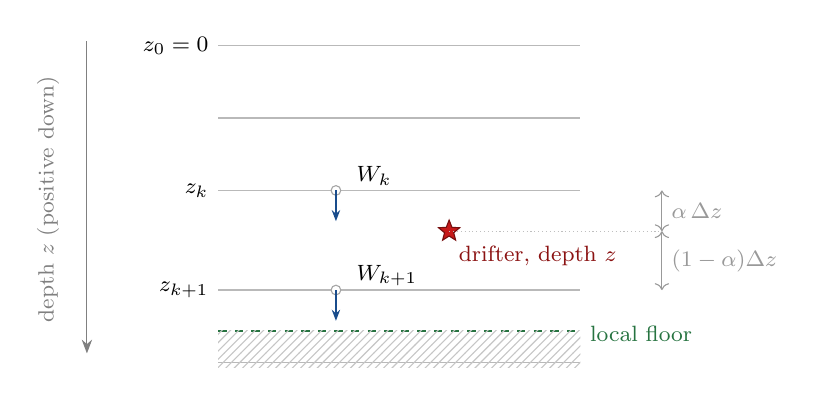
\begin{tikzpicture}[scale=1.15]
  \def\xl{0}\def\xr{4.0}
  \foreach \y in {0,-0.8,-1.6,-2.7,-3.5} \draw[interface] (\xl,\y)--(\xr,\y);
  \node[font=\footnotesize,left] at (\xl,0)    {$z_0=0$};
  \node[font=\footnotesize,left] at (\xl,-1.6) {$z_k$};
  \node[font=\footnotesize,left] at (\xl,-2.7) {$z_{k+1}$};
  \node[interfacept] at (1.3,-1.6) {}; \draw[velarrow] (1.3,-1.6)--++(0,-0.34);
  \node[font=\footnotesize,right] at (1.42,-1.44) {$\Wvel_k$};
  \node[interfacept] at (1.3,-2.7) {}; \draw[velarrow] (1.3,-2.7)--++(0,-0.34);
  \node[font=\footnotesize,right] at (1.42,-2.54) {$\Wvel_{k+1}$};
  \node[drifter] (D) at (2.55,-2.05) {};
  \node[font=\footnotesize,kelp!70!black,below right=2pt and 0pt] at (2.55,-2.05) {drifter, depth $\depx$};
  \draw[<->,gray!80] (4.9,-1.6)--(4.9,-2.05) node[midway,right,font=\footnotesize]{$\interpfrac\,\Delta z$};
  \draw[<->,gray!80] (4.9,-2.05)--(4.9,-2.7) node[midway,right,font=\footnotesize]{$(1-\interpfrac)\Delta z$};
  \draw[gray!50,densely dotted] (2.55,-2.05)--(4.9,-2.05);
  \draw[dashed,laggreen,line width=0.9pt] (\xl,-3.15)--(\xr,-3.15);
  \node[font=\footnotesize,laggreen,right] at (\xr,-3.18) {local floor};
  \fill[pattern=north east lines,pattern color=gray!45] (\xl,-3.15) rectangle (\xr,-3.55);
  \draw[-{Stealth[length=5pt]},gray] (-1.45,0.05)--(-1.45,-3.4);
  \node[gray,rotate=90,anchor=south,font=\footnotesize] at (-1.65,-1.7){depth $\depx$ (positive down)};
\end{tikzpicture}
\caption{Vertical interpolation of the vertical velocity, identical in form for the z-level and sigma
families. The interface values $\Wvel_k,\Wvel_{k+1}$ (open circles; downward arrows mark the
positive-down sign) bracket the drifter at depth $\depx$. The fraction
$\interpfrac=(\depx-z_k)/(z_{k+1}-z_k)$ is formed in physical depth, and the profile value is
$(1-\interpfrac)\Wvel_k+\interpfrac\Wvel_{k+1}$. No extrapolation is performed beyond the ends of the
column.}
\label{fig:vert}
\end{figure}

\codeanchor{The single-node profiles are \fn{\_interp\_w\_linear\_single} (z-level; the reusable
bracket is \fn{\_w\_bracket} with \fn{\_w\_at\_bracket}) and \fn{\_interp\_w\_sigma\_linear\_single}
(sigma), in \srcfile{numerics/vertical.py} and \srcfile{numerics/vertical\_sigma.py}.}

\section{Horizontal combination of the vertical velocity}\label{sec:vert-whoriz}

The profile of \cref{eq:vert-wlin} gives the vertical velocity at a single node; to obtain it at the
particle, the per-node profiles are combined horizontally over the one-ring of nodes surrounding the
particle. The combination method is selected by \conf{w\_interp}: \conf{nearest} (the profile at the
nearest node alone), \conf{leastsq} (a plane fit to the ring-node profiles, the default),
\conf{barycentric} (the vertex blend of \cref{ch:hvel} applied to the profiles), and \conf{idw}
(inverse-distance weighting). This least-squares stencil is over the surrounding \emph{nodes}, in
contrast to the horizontal velocity of \cref{sec:hvel-leastsq}, whose stencil is over the surrounding
\emph{element centres}; the two are distinct constructions that share a name. Only \conf{barycentric}
depends on the element type: on a quadrilateral it uses the Wachspress weights of
\cref{sec:hvel-quad}, on a triangle the triangular weights. The choice also decides whether a
three-dimensional run can use a fused kernel (\cref{ch:fused}).

\paragraph{z-level meshes.} When a profile is sampled at a neighbouring node, the evaluation depth is
capped at that neighbour's floor, $\depx_{\text{eval}}=\min(\depx,\,d_j)$, so that a shallow neighbour
cannot contribute a spurious below-floor velocity. The \conf{nearest} method evaluates the nearest
node's own profile without a cap: an RK stage position below that node's floor reads the profile below
the bottom, where the other methods' fallbacks cap the depth at the floor.

\paragraph{Sigma meshes.} On a sloping bottom a fixed depth cuts across sigma surfaces, and sampling
the neighbours at the particle's depth would mix the flow of different sigma levels. The neighbours
are therefore evaluated \emph{along the particle's sigma surface} (\cref{fig:vert-sigma}): with the
particle's fraction of its column
\begin{equation}\label{eq:vert-sigma-frac}
  \xi = \min\bigl(\max(\depx/H_p,\,0),\,1\bigr),
\end{equation}
neighbour $j$ is evaluated at $\depx_j=\xi\,H_j$, $H_j=\max(d_j+\eta_j,D_{\min})$. The particle column
$H_p$ is interpolated by the same method --- a least-squares plane (floored at $D_{\min}$), the
barycentric weights of the containing element, or inverse-distance weights --- which makes it exact for
a linearly sloping bottom under \conf{leastsq} and \conf{barycentric}; \conf{nearest} uses the nearest
node's column.

\begin{figure}[t]
\centering
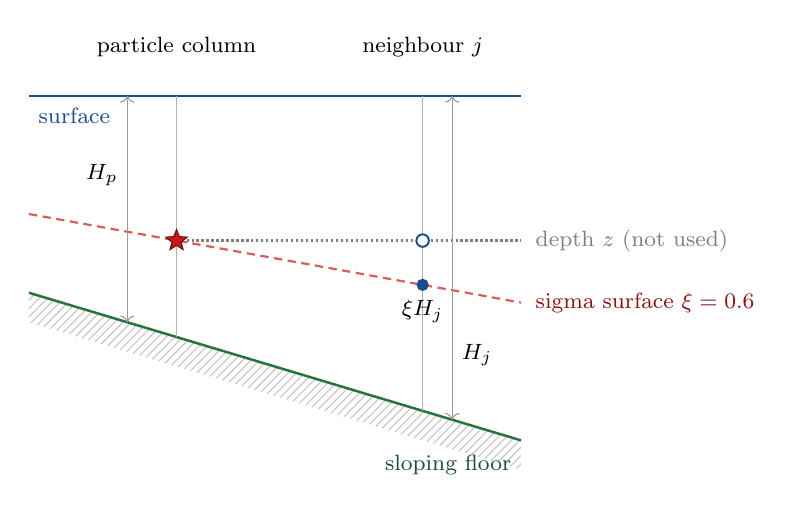
\begin{tikzpicture}[scale=1.25]
  \fill[pattern=north east lines,pattern color=gray!45] (0,-2.0)--(5,-3.5)--(5,-3.8)--(0,-2.3)--cycle;
  \draw[laggreen,line width=0.9pt] (0,-2.0)--(5,-3.5);
  \draw[lagblue,line width=0.9pt] (0,0)--(5,0);
  \node[font=\footnotesize,lagblue,anchor=north west] at (0,-0.02) {surface};
  \node[font=\footnotesize,laggreen!70!black,anchor=north east] at (5,-3.55) {sloping floor};
  \draw[gray!60] (1.5,0)--(1.5,-2.45);
  \draw[gray!60] (4.0,0)--(4.0,-3.2);
  \draw[kelp!70,densely dashed,line width=0.8pt] (0,-1.2)--(5,-2.1);
  \node[font=\footnotesize,kelp!70!black,anchor=west] at (5.05,-2.1) {sigma surface $\xi=0.6$};
  \draw[gray,densely dotted,line width=0.8pt] (1.5,-1.47)--(5,-1.47);
  \node[font=\footnotesize,gray,anchor=west] at (5.05,-1.47) {depth $\depx$ (not used)};
  \node[drifter] at (1.5,-1.47) {};
  \node[meshnode] at (4.0,-1.92) {};
  \node[meshnodeopen] at (4.0,-1.47) {};
  \draw[<->,gray!80] (1.0,0)--(1.0,-2.3) node[pos=0.35,left,font=\footnotesize,text=black]{$H_p$};
  \draw[<->,gray!80] (4.3,0)--(4.3,-3.29) node[pos=0.8,right,font=\footnotesize,text=black]{$H_j$};
  \node[font=\footnotesize,anchor=north] at (4.0,-1.98) {$\xi H_j$};
  \node[font=\footnotesize,anchor=south] at (1.5,0.3) {particle column};
  \node[font=\footnotesize,anchor=south] at (4.0,0.3) {neighbour $j$};
\end{tikzpicture}
\caption{Sigma-following evaluation of the vertical velocity. The particle sits at the fraction
$\xi=\depx/H_p$ of its column; the neighbouring column is evaluated at $\xi H_j$ on the same sigma
surface (filled node), not at the particle's depth (open node), which on a sloping floor lies on a
different sigma level.}
\label{fig:vert-sigma}
\end{figure}

Every method falls back to the nearest-node profile when its stencil is unusable, so the combined
vertical velocity is never undefined.

\codeanchor{The horizontal combinations are \fn{interp\_w\_spatial} (z-level) and
\fn{interp\_w\_sigma\_spatial} (sigma), in \srcfile{numerics/vertical.py} and
\srcfile{numerics/vertical\_sigma.py}; the particle column is \fn{sigma\_column\_height} with the
per-method helpers \fn{\_H\_leastsq\_single}, \fn{\_H\_bary\_single} and \fn{\_H\_idw\_single}.}

\section{The step on a sigma mesh}\label{sec:vert-sigma-step}

FESOM-C's vertical velocity is a flux through the sigma interfaces, not the rate of the particle's
depth: with the surface rising and falling and the floor sloping, a particle at rest on its sigma
surface still changes depth. The step therefore integrates the particle's fraction of the water column,
\begin{equation}\label{eq:vert-sigma-ode}
  \xi = \frac{\depx}{H_p}, \qquad \frac{d\xi}{dt}=\frac{\Wvel}{H_p},
\end{equation}
with $\Wvel$ the negated file value of \cref{tab:vert-wsign} (including the direction factor). With
$\xi_0=\depx_n/H_p(\mathbf{x}_0,t_0)$ and $f_k=\Wvel_k/H_{p,k}$ evaluated at stage $k$,
\begin{align}
  \text{Euler:}\quad & \xi_{n+1}=\xi_0+\dt\,f_1, \label{eq:vert-sigma-euler}\\
  \text{RK2:}\quad & \xi_{1/2}=\xi_0+\tfrac{\dt}{2}f_1,\qquad \xi_{n+1}=\xi_0+\dt\,f_2, \label{eq:vert-sigma-rk2}\\
  \text{RK4:}\quad & \xi_{n+1}=\xi_0+\tfrac{\dt}{6}\,(f_1+2f_2+2f_3+f_4). \label{eq:vert-sigma-rk4}
\end{align}
Every stage places the particle at $\depx=\xi\,H_p(\mathbf{x}_k,t_k)$ in the column at the stage position
and time, and the end of the step at $\depx_{n+1}=\xi_{n+1}\,H_p(\mathbf{x}_{n+1},t_{n+1})$. The surface
elevation at the start and at the end of every step comes from one function of time --- the PCHIP
value where a four-snapshot stencil exists and PCHIP is enabled, otherwise the linear blend, and in
discrete mode the next record --- so the end of one step and the start of the next see the same surface
bit for bit, $\xi$ is continuous across steps, and a resumed run reproduces the uninterrupted one. With a
linear time interpolant, a linear bottom and a uniform dia-sigma velocity the discrete solution is
exact; with a dia-sigma velocity linear in $\xi$ the three schemes converge at orders one, two and four.
The layer of the horizontal velocity, the depth clamp and the diffusion kicks (\cref{ch:diffusion}) use
the same column $H_p$. The recorded vertical velocity on a sigma mesh is $\Wvel$ itself, the dia-sigma
flux, not the rate of the particle's depth.

\codeanchor{The sigma branches of \fn{\_euler\_step\_unfused}, \fn{\_rk2\_step\_unfused} and
\fn{\_rk4\_step\_unfused} with the helpers \fn{\_sigma\_col\_H} and \fn{\_sigma\_end\_eta}
(\srcfile{numerics/integrators.py}); the surface at the step boundaries is \fn{\_eta\_at\_time}
(\srcfile{tracking.py}). Sigma meshes always take the unfused path (\cref{ch:fused}).}

\section{Depth clamping at the surface and the floor}\label{sec:vert-clamp}

After the vertical position is advanced, the depth is clamped into the admissible range, and the
limits differ by family. On a z-level mesh the depth is clamped into $[\,z_0,\ d_{\text{nn}}\,]$ --- the
surface interface and the per-node sea floor of the nearest node --- and neither $\eta$ nor any
minimum-thickness parameter enters. On a sigma mesh the depth is clamped into
$[\,0,\ \max(H_p-z_{0b},\,0)\,]$, with $H_p$ the end-of-step column at the particle and $z_{0b}$ (default
\SI{0.1}{\metre}) holding the particle a fixed distance above the bed. The clamp is applied at every
step, so a particle that reaches the floor is not removed but tracks along it, in contrast to a particle
that leaves the horizontal domain, which is flagged and removed (\cref{ch:lifecycle}).

\codenote{The keys \conf{Dmin} ($D_{\min}$) and \conf{z0b\_min} ($z_{0b}$) are consumed only on sigma
meshes; the z-level clamp uses neither (nor $\eta$). $z_{0b}$ is a geometric clamp offset, not a
roughness length in any physics. The sigma surface clamp holds the particle at a literal $\depx=0$
rather than at $(1-\sigma_0)H$, so it coincides with the top interface only when $\sigma_0=1$ exactly.}

\codeanchor{Depth clamping is \fn{clamp\_depth} (z-level, limits $[z_0,d_{\text{nn}}]$) and
\fn{clamp\_depth\_sigma} (sigma, limits $[0,\max(H_p-z_{0b},0)]$) in the respective vertical modules,
invoked by \fn{\_clamp\_z} (\srcfile{numerics/integrators.py}); the defaults
$D_{\min}=\SI{0.5}{\metre}$, $z_{0b}=\SI{0.1}{\metre}$ are set in \srcfile{core/config.py}.}

\chapter{Scalar Field Sampling Along Trajectories}\label{ch:sampling}

Beyond advecting particles, the engine can record the value of model scalar fields
--- temperature and salinity, for example --- at each
particle position as the trajectory unfolds. This sampling is a diagnostic: it does
not affect the motion, but it attaches a time series of water properties to every
trajectory. The fields to sample are listed in the configuration key
\conf{mode.sample\_vars} (a single name is accepted as a one-element list; an empty list switches
sampling off and leaves the output byte-identical), and the horizontal method in
\conf{numerics.sample\_interp}. This chapter
describes what is sampled, where in the column the value is taken, how the horizontal
combination reuses the interpolation machinery of \cref{ch:hvel,ch:vertical}, and why
sampling is deliberately independent of the integration direction.

\section{What is sampled, and when}\label{sec:samp-what}

The sampled fields are node-based scalars, read from the same forcing dataset as the
velocity. Each requested field is probe-read once at startup, before the output file is created; a
field that is absent, or that is stored at element centres rather than nodes, raises a configuration
error immediately rather than failing midway through a run. Each reader prepares the fields in its own
way: the FESOM2 reader recognises mid-layer and interface fields by their vertical dimension and picks
the tracked level in a two-dimensional run; the FESOM-C reader reduces sigma-layered fields to two
dimensions with a node-aware reduction in a two-dimensional run; the HEALPix reader compacts pixels to nodes and fills each
column downward from its deepest valid value, so that the bottom clamp reads bottom water, never a
missing value (pixel geometry does not support sampling); the NEMO reader samples surface T-point
fields only. Values are recorded at the
trajectory output cadence (every \conf{output\_freq} steps, \cref{ch:output}), not at
every integration step. A record is labelled with the time at the end of its step (\cref{eq:out-time}), and
the scalar is taken at that instant as far as the forcing allows. When the velocity is reconstructed in time
(\cref{ch:temporal}), the scalar is re-interpolated to the exact record time, so the
sampled value is consistent with the recorded position; this re-interpolation is linear between
the bracketing snapshots even when the velocity uses the monotone-cubic reconstruction. In the
discrete-time mode the scalar is read from the snapshot at the end of the step --- the next snapshot, which the
step already holds as the target of its Runge--Kutta stages --- so its instant is the record time as well.
Only when no next snapshot exists, on the last step of a run that stops at the end of the forcing, is the
snapshot at the start of the step used, one snapshot behind the record time; the variable's comment
attribute says so. (Before output format~2 the discrete mode always sampled the start-of-step snapshot.)

Each sampled field becomes a variable of the trajectory output with the dimensions of the positions,
filled with missing values before its first record and in any record that does not carry it, and carrying
the units and long name of the source variable, the positions as its coordinates, and a comment on the
sampling instant; names that collide with the output's own variables, the release variables included, are
refused. Checkpoints do not
store sampled values. A field read internally for beaching (\cref{ch:lifecycle}) is written only when it
is also listed in \conf{sample\_vars}. On a rotated mesh (\cref{ch:frame}) scalars are sampled in the
rotated frame and written as they are, which is correct for scalars; a vector component listed as a
sample stays in the rotated frame.

\section{Vertical placement by field shape}\label{sec:samp-shape}

The vertical treatment is selected by the shape of the field array, which encodes
where the field lives in the column. A two-dimensional field, one value per node, is
sampled horizontally only. A mid-layer field, with one value per layer per node, is
interpolated linearly between the two bracketing mid-layer depths --- the midpoints of
the layers, computed from the fixed interface depths on a z-level mesh or from the
column geometry of \cref{eq:sigma} on a sigma mesh, and clamped to the first and last midpoint. On a
z-level mesh each neighbour is evaluated no deeper than its own floor, as for the vertical velocity
(\cref{sec:vert-whoriz}). On a sigma mesh each neighbour column is evaluated at the particle's
\emph{depth}, capped at the column thickness, and not along the particle's sigma surface as the
vertical velocity is; on a sloping bottom the sample therefore mixes neighbouring sigma levels, a
limitation that remains to be removed. An interface field, with one value per interface per node, is
handled by delegating to the vertical-velocity machinery of \cref{sec:vert-wprofile,sec:vert-whoriz},
including its sigma-following evaluation. In that delegation the integration-direction
factor is fixed to $+1$, for the reason given in \cref{sec:samp-direction}.

\section{Horizontal combination and element type}\label{sec:samp-horiz}

The horizontal combination offers the same four methods as the vertical velocity ---
\conf{nearest}, \conf{leastsq}, \conf{barycentric}, and \conf{idw} --- and shares their
behaviour with respect to the mesh. As with the vertical velocity, only the
\conf{barycentric} method depends on the element type, using the Wachspress weights of
\cref{sec:hvel-quad} on a quadrilateral and the triangular weights on a triangle; the
other three combine surrounding node values irrespective of element shape. Each method
falls back to the nearest node's value when its stencil is unusable. A particle that is not alive
(including a beached or a not-yet-released one) and a particle without a nearest node are recorded as
missing.

Model fields often carry fill values at coastal or below-bottom nodes, and a linear combination would
propagate them. The fitting methods therefore skip non-finite neighbours: the least-squares fit uses
the finite ones and needs at least three; inverse-distance weighting drops them; a barycentric element
with a non-finite vertex falls back to the nearest node's value. Under \conf{nearest}, and under
\conf{idw} for a particle that coincides with a node, the sample is that node's raw value, a fill value
included, because the sample point then \emph{is} that node; the least-squares fit has no such case and
returns the plane through the finite neighbours even at a node. Interface fields, which go through the vertical-velocity
machinery, are not filtered.

\section{Independence from the integration direction}\label{sec:samp-direction}

Sampling is a measurement of the instantaneous field and must not change sign when the
run is integrated backward in time. The engine enforces this by fixing the
direction factor to $+1$ in the sampling path, in contrast to the advection path, where
the factor $\tdir$ carries the forward or backward direction into the interpolated
velocity (\cref{sec:arch-direction}). The distinction matters specifically for an
interface-located scalar, which is sampled through the vertical-velocity machinery:
without the override it would inherit the velocity's direction sign and report a
sign-flipped value on a backward run. A sampled temperature is a temperature regardless
of the direction of integration.

\codeanchor{Sampling is implemented in \fn{sample\_field} and the direction-free combine
\fn{\_combine\_horizontal} (\srcfile{numerics/sampling.py}); the per-record sampling is
driven by \fn{\_sample\_record\_fields} (\srcfile{tracking.py}); each reader's
\fn{read\_scalar\_fields} prepares the fields and serves the startup probe.}

\chapter{Coordinate Frame and Rotation}\label{ch:frame}

A global ocean mesh must contend with the convergence of the meridians at the geographic poles, where
the longitude metric $\zzero=\cos\latx\,\Mlat$ of \cref{sec:intro-conv} vanishes and longitude becomes
ill-conditioned. FESOM2 meshes commonly avoid this by rotating the computational frame so that its
poles lie over land --- conventionally over Greenland and Antarctica --- leaving the entire ocean far from
the coordinate singularity. This chapter describes how the engine supports such a rotated frame: the
rotation itself, the distinction between rotating points and rotating vectors, what is and is not
affected, the contract that keeps the rotation invisible to the user, and the accuracy it achieves. The
facility is available on FESOM2 and HEALPix meshes; FESOM-C meshes and NEMO-derived meshes reject a
non-null \conf{mesh.rotation} with a configuration error.

\section{The rotated frame}\label{sec:frame-rotation}

The rotation is configured by the key \conf{mesh.rotation}. Its default is \conf{null}, a geographic
frame in which no rotation is applied and the trajectories are computed directly in longitude and
latitude; a run with this default is byte-identical to one on an engine without the facility. Setting
\conf{mesh.rotation} to \conf{fesom2} selects FESOM2's own Euler angles $(\alpha,\beta,\gamma)=
(50^\circ,15^\circ,-90^\circ)$, which place the computational poles in Greenland and in East Antarctica;
an explicit triple of angles may also be given. The rotation is a rigid map of the sphere,
\begin{equation}\label{eq:frame-map}
  \mathbf{r}' = \mathbf{R}(\alpha,\beta,\gamma)\,\mathbf{r},\qquad
  \mathbf{r}=(\cos\latx\cos\lonx,\ \cos\latx\sin\lonx,\ \sin\latx),
\end{equation}
with $\mathbf{R}$ the Euler rotation matrix and $\mathbf{R}^{\mathsf T}$ its inverse; rotated longitudes are
wrapped to $[-180^\circ,180^\circ)$. It is applied once when the mesh and each velocity snapshot are read,
never inside the per-particle loop. With the \conf{fesom2} angles the rotated FESOM2 mesh reproduces the
model's own element areas to machine precision.

\section{Rotating points and rotating vectors}\label{sec:frame-vectors}

The rotation acts differently on positions and on velocities, and the distinction is essential to
correctness (\cref{fig:rotation}). Node coordinates and element centres are \emph{points}: they are
mapped by \cref{eq:frame-map}. The element centres are rotated as points and not recomputed from the
rotated nodes, because a centroid computed on the sphere does not commute with the rotation. The
horizontal velocity components, by contrast, are the components of a \emph{tangent vector} expressed in
the local east--north frame, and that local frame itself turns from place to place; the velocity must
therefore be re-expressed in the rotated frame's local east--north basis. With $c$ and $s$ the cosine
and sine of the local angle through which the unit-east direction turns, the transformed components are
\begin{equation}\label{eq:vec-rot}
  u' = c\,u - s\,v, \qquad v' = s\,u + c\,v,
\end{equation}
a rotation that preserves the speed, $u'^2+v'^2=u^2+v^2$. The factors $(c,s)$ are the rotated-frame
components of $\mathbf{R}\,\hat{\mathbf{e}}$, with $\hat{\mathbf{e}}=(-\sin\lonx,\cos\lonx,0)$ the geographic
unit east vector, computed once per velocity carrier --- per node, per element centre, or both, as the
mesh's velocity layout requires --- from the \emph{geographic} coordinates, before the points are
rotated. At an exact pole the east direction is taken as the limit at the stored longitude.

Scalar and vertical quantities have no horizontal direction and pass through unchanged: the vertical
velocity, the sea-surface height, the diffusivity and the sampled scalars. For the diffusivity one
qualification applies: a diffusivity whose zonal and meridional values differ acts along the rotated
axes rather than along east and north, and the engine warns once when it meets such a pair. The
stochastic kicks move along great circles (\cref{ch:diffusion}), so an isotropic diffusivity gives the
same statistics in either frame.

\begin{figure}[t]
\centering
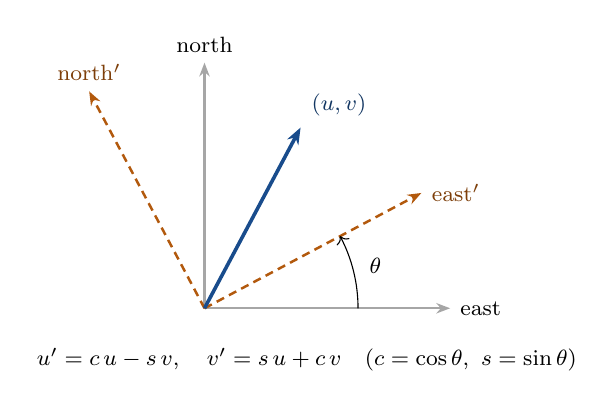
\begin{tikzpicture}[scale=1.3]
  \coordinate (O) at (0,0);
  \def\th{28}
  \draw[-{Stealth[length=5pt]},gray!70,line width=0.8pt] (O)--(2.4,0) node[right,font=\footnotesize,black]{east};
  \draw[-{Stealth[length=5pt]},gray!70,line width=0.8pt] (O)--(0,2.4) node[above,font=\footnotesize,black]{north};
  \draw[-{Stealth[length=5pt]},lagelem,line width=0.9pt,densely dashed] (O)--(\th:2.4) node[right,font=\footnotesize,lagelem!70!black]{east$'$};
  \draw[-{Stealth[length=5pt]},lagelem,line width=0.9pt,densely dashed] (O)--({\th+90}:2.4) node[above,font=\footnotesize,lagelem!70!black]{north$'$};
  \draw[->,black] (1.5,0) arc (0:\th:1.5);
  \node[font=\footnotesize] at ({\th/2}:1.72) {$\theta$};
  \draw[-{Stealth[length=6pt]},lagblue,line width=1.3pt] (O)--(62:2.0) node[above right,font=\footnotesize,lagblue!70!black]{$(u,v)$};
  \node[font=\footnotesize] at (1.0,-0.5) {$u'=c\,u-s\,v,\quad v'=s\,u+c\,v\quad(c=\cos\theta,\ s=\sin\theta)$};
\end{tikzpicture}
\caption{Rotation of a horizontal velocity into the rotated frame. The velocity $(u,v)$ is a tangent
vector; its components are re-expressed in the rotated local east--north basis (dashed), turned through
the local angle $\theta$, by \cref{eq:vec-rot}. The map preserves the speed. Node coordinates and element
centres, being points rather than vectors, are instead mapped directly by the rotation.}
\label{fig:rotation}
\end{figure}

\section{The user-facing contract}\label{sec:frame-contract}

The rotation is arranged to be invisible outside the engine. Release positions are always supplied in
geographic coordinates and are rotated into the computational frame when the run starts. Trajectory
output is always geographic: at every record the positions and the horizontal velocity diagnostics are
un-rotated on a copy of the state, while the internal state stays in the rotated frame; the vertical
velocity and the sampled scalars are written as they are. The release positions written with the
trajectories (\cref{sec:out-schema}) are geographic too: the particle state carries them in the rotated
frame, checkpoints store them in that frame, and they are un-rotated by the same rule when they are
written. A restart checkpoint records the three angles
of the frame in which it was written, and a resuming driver validates them against the mesh
(\fn{\_validate\_restart\_frame}, \cref{ch:output}), so a run is not continued in a different frame by
accident; the output file carries the angles as metadata whenever
the frame is rotated. Within this contract the rotation is purely an internal device for conditioning
the arithmetic near the poles. Periodic fold windows (\cref{ch:lifecycle}) are defined in the mesh's
coordinates and cannot be combined with a rotation; the combination is refused.

\section{Rotation on HEALPix meshes}\label{sec:frame-healpix}

A FESOM2 model builds its mesh in its own rotated frame; a HEALPix product carries geographic east and
north components on a global pixel grid. Rotation of a HEALPix mesh is therefore a pure runtime
transform: node coordinates are rotated as points, the velocities receive tangent factors per node (per pixel centre on the pixel mesh), the
search structures are rebuilt on the rotated coordinates, and the tracking layer handles the rest as for
FESOM2. The rotated frame has two poles of its own, and the polar pathologies move there, so the loader
guards against them: a wet element that straddles a rotated pole is refused with an error that names
where the poles land, and wet nodes poleward of $88^\circ$ rotated latitude produce a warning. With the
\conf{fesom2} angles both poles fall on land, and on the global HEALPix products tested the wet nodes stay
below about $85^\circ$ rotated latitude. In the geographic frame, by contrast, the containment test rejects
points poleward of the first ring of pixel centres, $\arcsin\bigl(1-1/(3\,n_{\text{side}}^2)\bigr)$ ---
$84.15^\circ$ at $n_{\text{side}}=8$, $89.91^\circ$ at $n_{\text{side}}=512$ --- so a particle there dies
as \code{OUTSIDE}; for global HEALPix runs the rotation is the recommended setting.

\section{Accuracy and when rotation is needed}\label{sec:frame-accuracy}

Rotation is a change of chart, not of physics, and away from the poles a correctly implemented run
differs between the geographic and rotated frames only at the level of the discretization. In the
engine's verification the two frames agree to about $10^{-6}$ degrees at mid-latitudes, and the
difference shrinks as the step is refined: at second order in the step for element-layout velocity and
at first order for node-layout velocity. Across a pole only the rotated frame can track: a meridional
flow over the pole follows the analytic great circle to within \SI{7e-8}{\metre}, whereas the geographic
frame breaks down there. A genuine framing error would produce discrepancies of tens of degrees,
independent of the step. Over long integrations the two frames diverge like any two slightly different
discretizations of a chaotic flow; their statistics, not their individual paths, are what agree.

Rotation becomes necessary only when the mesh carries wet points close to a geographic pole. The
FESOM2 reader warns, and suggests the \conf{fesom2} setting, when a mesh extends beyond about
$\pm 88^{\circ}$ without a rotation, and warns about a node exactly at a pole when rotated; the FESOM-C
reader warns without the suggestion; the HEALPix reader warns as described in \cref{sec:frame-healpix}.
For regional domains away from the poles the geographic frame is appropriate and is the default.

\codeanchor{The maps are \fn{euler\_matrix}, \fn{rotate\_lonlat}/\fn{unrotate\_lonlat} and
\fn{rotate\_vectors}/\fn{unrotate\_vectors} in \srcfile{core/rotation.py}; the angles and vector factors
are \fn{rotation\_angles} and \fn{\_vec\_rot\_factors} (\srcfile{core/mesh.py}); the readers apply them
in \fn{\_apply\_mesh\_rotation} (\srcfile{readers/fesom2.py}) and \fn{\_apply\_rotation}
(\srcfile{readers/healpix.py}); the tracking layer rotates seeds in \fn{\_maybe\_rotate\_seeds},
un-rotates records in \fn{\_geo\_view\_for\_record} and checks restarts in
\fn{\_validate\_restart\_frame} (\srcfile{tracking.py}).}


\part{Time Integration}
\chapter{Time-Integration Schemes}\label{ch:integration}

With the velocity available at an arbitrary position and time (\crefrange{ch:hvel}{ch:temporal}),
the engine advances the trajectory equation \cref{eq:lagrangian-ode} by an explicit
time-integration scheme. Four are provided, selected by \conf{numerics.integrator}: the
first-order Euler method, the second-order midpoint Runge--Kutta method (RK2), the
classical fourth-order Runge--Kutta method (RK4) \citep{butcher2016numerical}, and an adaptive
Dormand--Prince 5(4) method (RK45) \citep{dormand1980family} that subdivides each step to an error
tolerance. This chapter gives the discrete position update common to all of them, the per-scheme
stage formulae as implemented, what happens when a stage fails, and the way the integration
direction enters. The interaction
of scheme order with the temporal reconstruction --- which can cap the achievable order
--- is the subject of \cref{ch:temporal}.

\section{The displacement metric}\label{sec:int-metric}

The velocity is in metres per second but the horizontal position is in degrees, so each
update converts through the spherical metric of \cref{sec:intro-conv}. A horizontal
velocity $(U,V)$ over a step $\dt$ displaces the particle by
\begin{equation}\label{eq:int-displacement}
  \Delta\lonx = \frac{\dt\,U}{\zzero}, \qquad
  \Delta\latx = \frac{\dt\,V}{\Mlat}, \qquad
  \Delta\depx = \Wvel\,\dt,
\end{equation}
with $\Mlat=\SI{111120}{\metre\per\degree}$ the metres per degree of latitude and
$\zzero=\max(\cos\latx\,\Mlat,\,1)$ the metres per degree of longitude. The lower bound
of \SI{1}{\metre\per\degree} on $\zzero$ is a guard against the cosine vanishing at the
poles; longitude is wrapped to $[-180^{\circ},180^{\circ})$ and latitude is held within
$[-90^{\circ},90^{\circ}]$ after each update, for the stage positions and for the particles that
moved --- the positions of dead and not-yet-released particles are returned unchanged. The interpolated velocity already carries
the integration-direction factor $\tdir$ (\cref{sec:arch-direction}), so the time step
$\dt$ in \cref{eq:int-displacement} is always positive and the same formulae serve
forward and backward integration.

\section{The three schemes}\label{sec:int-schemes}

\paragraph{Euler.} The Euler step evaluates the velocity once, at the current position,
and applies \cref{eq:int-displacement} directly:
\begin{equation}\label{eq:euler}
  \pos_{n+1} = \pos_n + \Delta\pos\bigl(\velvec(\pos_n,t_n)\bigr).
\end{equation}
It is first-order accurate: the error per step is of order $\dt^2$.

\paragraph{RK2 (midpoint).} The midpoint method evaluates the velocity twice. A first
evaluation at the current position gives a provisional half-step displacement to a
midpoint; the velocity is then evaluated at that midpoint, at the half-step time, and
the full step uses this midpoint velocity:
\begin{align}\label{eq:rk2}
  (U_1,V_1) &= \velvec(\pos_n,t_n), &
  \pos_{\text{mid}} &= \pos_n + \tfrac{1}{2}\Delta\pos(U_1,V_1), \notag\\
  (U_2,V_2) &= \velvec(\pos_{\text{mid}},\,t_n+\tfrac{1}{2}\dt), &
  \pos_{n+1} &= \pos_n + \Delta\pos(U_2,V_2).
\end{align}
The longitude metric of each displacement is taken at the latitude where its velocity was evaluated:
$\zzero(\latx_n)$ for the half step and $\zzero(\latx_{\text{mid}})$ for the full step,
$\Delta\lonx=\dt\,U_2/\zzero(\latx_{\text{mid}})$. With the metric of the starting latitude the
longitude update would fall to first order; the scheme is second-order accurate.

\paragraph{RK4 (classical).} The fourth-order method evaluates the velocity at four
stages and combines their displacements with the classical weights $\tfrac16(1,2,2,1)$
(\cref{fig:rk4}). Writing the per-stage degree increment as
$\mathbf{d}_k=\Delta\pos(U_k,V_k)$, the stages are
\begin{align}\label{eq:rk4}
  \mathbf{d}_1 &= \Delta\pos\bigl(\velvec(\pos_n,\,t_n)\bigr), &
  \mathbf{d}_2 &= \Delta\pos\bigl(\velvec(\pos_n+\tfrac12\mathbf{d}_1,\,t_n+\tfrac12\dt)\bigr), \notag\\
  \mathbf{d}_3 &= \Delta\pos\bigl(\velvec(\pos_n+\tfrac12\mathbf{d}_2,\,t_n+\tfrac12\dt)\bigr), &
  \mathbf{d}_4 &= \Delta\pos\bigl(\velvec(\pos_n+\mathbf{d}_3,\,t_n+\dt)\bigr),
\end{align}
and the position advances by
\begin{equation}\label{eq:rk4-combine}
  \pos_{n+1} = \pos_n + \tfrac{1}{6}\bigl(\mathbf{d}_1 + 2\mathbf{d}_2 + 2\mathbf{d}_3 + \mathbf{d}_4\bigr).
\end{equation}
The longitude metric $\zzero$ is recomputed at each stage's latitude. RK4 is fourth-order accurate in
space.

In three dimensions on a z-level mesh the depth is advanced by the same stage structure, with
$\Delta\depx_k=\Wvel_k\,\dt$ (for RK2, $\depx_{\text{mid}}=\depx_n+\Wvel_1\dt/2$ and
$\depx_{n+1}=\depx_n+\Wvel_2\dt$), without clamping between stages, and the depth is clamped to the
column after the step (\cref{sec:vert-clamp}). On a sigma mesh the stages advance the particle's
fraction of the water column instead (\cref{sec:vert-sigma-step}).

\begin{figure}[t]
\centering
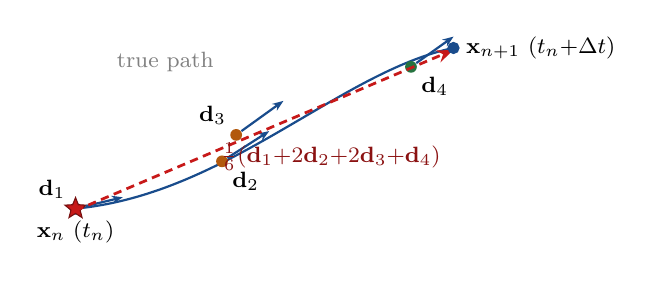
\begin{tikzpicture}[scale=1.2]
  \draw[thick,lagblue] (0,0) .. controls (1.6,0.15) and (2.8,1.45) .. (4.0,1.7);
  \node[meshnode] at (0,0) {};
  \node[font=\footnotesize,below=1pt] at (0,0) {$\pos_n$ ($t_n$)};
  % stage points
  \node[drifter] (k1) at (0,0) {};
  \node[circle,fill=lagelem,inner sep=1.5pt] (k2) at (1.55,0.5) {};
  \node[circle,fill=lagelem,inner sep=1.5pt] (k3) at (1.7,0.78) {};
  \node[circle,fill=laggreen,inner sep=1.5pt] (k4) at (3.55,1.5) {};
  \node[font=\footnotesize,above left=-2pt of k1] {$\mathbf{d}_1$};
  \node[font=\footnotesize,below right=-2pt of k2] {$\mathbf{d}_2$};
  \node[font=\footnotesize,above left=-2pt of k3] {$\mathbf{d}_3$};
  \node[font=\footnotesize,below right=-2pt of k4] {$\mathbf{d}_4$};
  % slope arrows
  \foreach \p/\dx/\dy in {k1/0.5/0.12,k2/0.5/0.32,k3/0.5/0.36,k4/0.45/0.32}
     \draw[velarrow] (\p)--++(\dx,\dy);
  % final weighted step
  \draw[-{Stealth[length=6pt]},densely dashed,kelp,line width=1pt] (0,-0.02)--(4.0,1.68);
  \node[font=\footnotesize,kelp!70!black] at (2.7,0.55) {$\tfrac16(\mathbf{d}_1{+}2\mathbf{d}_2{+}2\mathbf{d}_3{+}\mathbf{d}_4)$};
  \node[meshnode] at (4.0,1.7) {};
  \node[font=\footnotesize,right=1pt] at (4.0,1.7) {$\pos_{n+1}$ ($t_n{+}\dt$)};
  \node[font=\footnotesize,gray] at (0.95,1.55) {true path};
\end{tikzpicture}
\caption{The four stages of RK4. The slope $\mathbf{d}_1$ is sampled at the start
($t_n$); $\mathbf{d}_2$ and $\mathbf{d}_3$ at provisional midpoints (time
$t_n+\tfrac12\dt$); $\mathbf{d}_4$ at a provisional endpoint ($t_n+\dt$). The step is
their weighted average \cref{eq:rk4-combine} (dashed), a fourth-order approximation to
the true path (blue). Each stage requires the velocity at a different position
\emph{and} time, which is why the temporal reconstruction of \cref{ch:temporal} matters.}
\label{fig:rk4}
\end{figure}

\section{The adaptive scheme}\label{sec:int-rk45}

With \conf{integrator: rk45} each particle subdivides the tracking step $\dt$ into substeps $h$ chosen
by an error estimate, using the Dormand--Prince 5(4) pair with the coefficients of MATLAB's
\code{ode45}. The right-hand side is $(\dot\lonx,\dot\latx)=(U/\zzero,\,V/\Mlat)$; each stage samples the
velocity at its own time through the same nested temporal blend as the fused kernels
(\cref{sec:fused-identity}). The difference between the fifth- and fourth-order solutions is converted to
metres,
\begin{equation}\label{eq:rk45-err}
  e=\sqrt{\bigl(e_\lonx\,\zzero\bigr)^2+\bigl(e_\latx\,\Mlat\bigr)^2},
\end{equation}
and a substep is accepted when $e$ does not exceed \conf{rk45\_tol\_m} (default \SI{1}{\metre}). After
every attempt, accepted or rejected, the substep becomes
\begin{equation}\label{eq:rk45-control}
  h \leftarrow h\cdot\min\bigl(\max\bigl(0.9\,(\mathrm{tol}/e)^{1/5},\,0.2\bigr),\,5\bigr),
\end{equation}
the first attempt is the whole step, the last substep is clipped to end exactly at $\dt$, and the last
stage of an accepted substep is reused as the first of the next. Apart from the last one, clipped to the end of the step, a
substep is never smaller than \conf{rk45\_h\_min} (default $10^{-4}\dt$): a substep at that floor is accepted even above the tolerance,
and the run warns with the number of such substeps. A failed stage interpolation counts as a rejected
attempt and retries at a fifth of the substep; only a failure at the floor, or more attempts than
$\max(10^4,\ 2\,\dt/h_{\min}+16)$, ends the particle.

The adaptive scheme has a single fused kernel and no unfused twin, and its first version is limited to
two-dimensional runs with element-layout least-squares interpolation, without the monotone-cubic time
reconstruction, element tracking, or spatially varying diffusivity; each excluded combination is refused
before the output file is created. The tolerance, and the floor when it is set, are written to the output
metadata.

\section{Failure within a step}\label{sec:int-failure}

A stage whose interpolation fails --- no fit, no containing element --- ends the step for that particle:
it is returned to its position at the start of the step, with its starting nearest node, its status is set
to \code{OUTSIDE} and its failure reason to an interpolation failure. Stage positions are not tested for
containment; only the final position is, and a final position outside every element fails the same way
with the reason out of bounds (\cref{ch:lifecycle}). The velocity recorded with the particle is that of
the first stage --- the velocity at the start of the step --- for Euler, RK2 and RK4, and that at the end of
the last substep for RK45.

\section{Order, and what limits it}\label{sec:int-order}

The nominal orders --- one, two, and four --- are spatial: they describe how the error falls as the step
shrinks, provided the velocity is known exactly as a function of time. In practice the velocity is
reconstructed between stored snapshots, and the accuracy of that reconstruction in time can become the
binding constraint. As we show in \cref{ch:temporal}, a linear-in-time reconstruction caps the
time-truncation error at second order regardless of the spatial scheme, so that RK4 delivers no advantage
over RK2 unless either the step is much smaller than the snapshot interval or a higher-order temporal
reconstruction is used. The adaptive scheme controls the local error of the trajectory for the velocity
field as reconstructed; it cannot recover accuracy that the reconstruction in time does not carry. We
therefore defer any claim about realized accuracy to that chapter.

\codeanchor{The schemes are \fn{euler\_step}, \fn{rk2\_step}, \fn{rk4\_step} and \fn{rk45\_step} (kernel
\fn{\_rk45\_kernel\_2d}, stage evaluation \fn{\_rk45\_eval}), dispatched by \fn{get\_integrator}; the
update equations \crefrange{eq:int-displacement}{eq:rk4-combine} are implemented in the kernels of
\srcfile{numerics/integrators.py}, with the metric in \srcfile{core/geometry.py}.}

\chapter{Temporal Reconstruction of the Velocity Field}\label{ch:temporal}

The integration schemes of \cref{ch:integration} require the velocity not only at
arbitrary positions but at arbitrary times --- at the half-step and full-step instants
of the Runge--Kutta stages --- whereas the model stores it only at discrete snapshots.
The engine bridges this gap by reconstructing the velocity in time between snapshots.
This chapter describes the two modes of operation (one snapshot per step, or
sub-stepping with interpolation), the linear and monotone-cubic reconstructions, and the
central consequence that the temporal reconstruction can cap the order of the spatial
scheme. The handling of the snapshot times themselves --- including the shift applied to
time-averaged forcing --- belongs to the forcing reader and is described in
\cref{ch:input}.

\section{Discrete and interpolated modes}\label{sec:temp-modes}

The key \conf{temporal\_interp} selects between two modes. In the \emph{discrete} mode (the default),
each integration step advances by one stored snapshot; the displacement uses the step \conf{numerics.dt},
which must therefore equal the record spacing (taken from the file's time axis when it is not set; a
different step, or irregular record times such as calendar months, are refused when the run starts), and
the Runge--Kutta stages are
still ordered in time, the next snapshot being supplied so that the stages see the correct time
progression across the step. In the \emph{interpolated} mode, the time step may be smaller than the
snapshot interval, and the velocity at each stage time is reconstructed from the bracketing snapshots.
Sub-stepping in the interpolated mode is the means by which a fine step can be taken against coarsely
sampled forcing, for example a sub-daily step against daily-mean fields. The interpolated mode needs a
physical time axis: a file without a decodable time coordinate is refused unless the snapshot spacing
is given as \conf{numerics.file\_dt}.

\section{Linear reconstruction}\label{sec:temp-linear}

The default reconstruction is linear in time. For a time $t$ falling between snapshots at $t_a$ and $t_b$
carrying velocity fields $\velvec_a$ and $\velvec_b$, the reconstructed field is
\begin{equation}\label{eq:temp-linear}
  \velvec(t) = (1-\interpfrac)\,\velvec_a + \interpfrac\,\velvec_b, \qquad
  \interpfrac = \frac{t-t_a}{t_b-t_a}.
\end{equation}
A step starting at $t$ between two snapshots receives the field at its start, with
$\interpfrac_0=(t-t_a)/(t_b-t_a)$, and a \emph{target} snapshot $\velvec_T$ toward which its stages
move: the next snapshot, $t_b$, when integrating forward, and the previous one, $t_a$, when integrating
backward; a backward step that starts exactly on a snapshot brackets downward, so it has a real target
rather than none. The stage with time fraction $c_k$ (\cref{sec:int-schemes}) samples
\begin{equation}\label{eq:temp-stage}
  \velvec_k=(1-\interpfrac_k)\,\velvec(t)+\interpfrac_k\,\velvec_T,\qquad
  \interpfrac_k=\frac{c_k\,\dt}{\Delta t_T},
\end{equation}
with $\Delta t_T$ the time from the step's start to the target snapshot; \cref{eq:temp-stage} is
\cref{eq:temp-linear} evaluated at $t\pm c_k\dt$. The engine never forms $\velvec(t)$ as a whole field
unless a consumer asks for it: the velocity handed to a step between two snapshots is a lazy view that
blends a field on its first use, and the fused kernels blend each element or vertex they read
(\cref{eq:fused-nested}).

A step longer than the time to its target snapshot, $\dt>\Delta t_T$, would place its later stages
beyond the bracketing pair. Such a step runs on a steady velocity --- the field at its start --- and the
engine warns once per realization and reports the number of such steps at the end of a verbose run.
This happens at the end of the record, on a start between snapshots, and whenever $\dt$ does not
divide the snapshot interval: every step that straddles a snapshot then runs steady.

\section{The order cap, and monotone-cubic reconstruction}\label{sec:temp-pchip}

A linear reconstruction in time is itself only second-order accurate, and this caps the
\emph{time}-truncation error of the whole integration at order $\dt^2$ irrespective of
the spatial scheme. The practical consequence is important: under linear reconstruction,
RK4 collapses onto RK2 --- the fourth-order spatial scheme delivers no benefit --- unless
the step is taken much smaller than the snapshot interval. The remedy, short of finer
sub-stepping, is a higher-order reconstruction in time, selected by
\conf{temporal\_reconstruction}${}={}$\conf{pchip}.

The PCHIP reconstruction (\cref{fig:temporal}) fits a monotone piecewise-cubic Hermite
interpolant \citep{fritsch1980monotone} through four consecutive snapshots
$t_{n-1},t_n,t_{n+1},t_{n+2}$, evaluating it within the central interval
$[t_n,t_{n+1}]$. On that interval, with local coordinate $s=(t-t_n)/h_1$ and
$h_1=t_{n+1}-t_n$, the value is the Hermite combination
\begin{equation}\label{eq:pchip}
  f(t) = h_{00}(s)\,f_n + h_{10}(s)\,h_1 m_n + h_{01}(s)\,f_{n+1} + h_{11}(s)\,h_1 m_{n+1},
\end{equation}
with the standard cubic basis $h_{00}=2s^3-3s^2+1$, $h_{10}=s^3-2s^2+s$,
$h_{01}=-2s^3+3s^2$, $h_{11}=s^3-s^2$. The slope at an interior snapshot is the weighted harmonic
mean of the two adjacent secants $d_-$ and $d_+$ over intervals $h_-$ and $h_+$
\citep{fritsch1984method},
\begin{equation}\label{eq:pchip-slope}
  m=\frac{w_1+w_2}{w_1/d_-+w_2/d_+},\qquad w_1=2h_++h_-,\quad w_2=h_++2h_-,
\end{equation}
and zero wherever the two secants differ in sign or either vanishes. This makes the interpolant
monotone between samples and prevents the spurious overshoots that an unconstrained cubic would
introduce. The property holds for each component separately: the cubic does not preserve linear
relations between components or between snapshots --- a vanishing divergence, rotation equivariance, a
window mean --- which the linear reconstruction does preserve. Because the reconstruction is now cubic in time, the fourth-order spatial
scheme is no longer masked: RK4 separates from RK2 at coarse snapshot cadence. The PCHIP
stencil requires four consecutive snapshots, so on the first and last interval of the
record, and across a cyclic seam, the engine falls back to the linear reconstruction, with one warning
per realization. The reconstruction applies to the horizontal and vertical velocity and the sea-surface
height; the diffusivities stay linear in time, and sampled scalars are re-interpolated linearly to
the record time (\cref{sec:samp-what}). PCHIP is active
only with \conf{temporal\_interp: true} (otherwise it warns that it has no effect) and only for the
multistage schemes RK2 and RK4; the Euler step has no stage times to reconstruct.

The two-dimensional least-squares kernels and the three-dimensional barycentric RK2 kernel evaluate the
cubic inline for each element or vertex they read (\cref{ch:fused}). Every other configuration
reconstructs whole fields at each distinct stage time --- the two midpoint stages of RK4 share one ---
with a parallel loop over the field that is bit-identical to the plain array expression; one such blend
of a global field takes about \SI{46}{ms} at eight threads.

\begin{figure}[t]
\centering
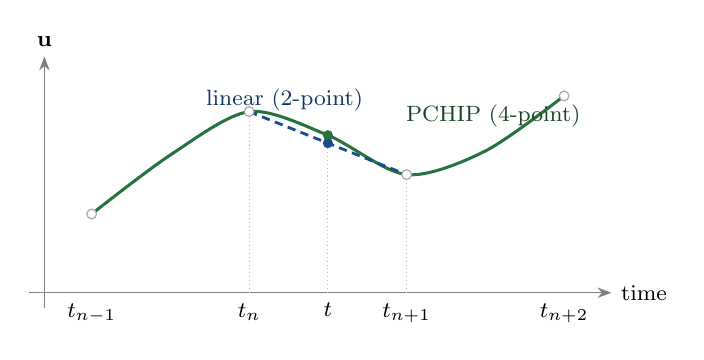
\begin{tikzpicture}[scale=1.0]
  % axes
  \draw[-{Stealth[length=5pt]},gray] (-0.2,0)--(7.2,0) node[right,font=\footnotesize,black]{time};
  \draw[-{Stealth[length=5pt]},gray] (0,-0.2)--(0,3.0) node[above,font=\footnotesize,black]{$\velvec$};
  % snapshot points
  \coordinate (s0) at (0.6,1.0);
  \coordinate (s1) at (2.6,2.3);
  \coordinate (s2) at (4.6,1.5);
  \coordinate (s3) at (6.6,2.5);
  % PCHIP smooth curve through all four
  \draw[laggreen,line width=1.1pt,smooth] plot coordinates {(0.6,1.0) (1.6,1.75) (2.6,2.3) (3.6,2.0) (4.6,1.5) (5.6,1.8) (6.6,2.5)};
  % linear chord on central interval [t_n, t_{n+1}] = s1..s2
  \draw[lagblue,line width=1.0pt,densely dashed] (s1)--(s2);
  % central interval shading
  \draw[gray!55,densely dotted] (2.6,0)--(2.6,2.3);
  \draw[gray!55,densely dotted] (4.6,0)--(4.6,1.5);
  % query substep
  \coordinate (q) at (3.6,0);
  \draw[gray!55,densely dotted] (3.6,0)--(3.6,2.02);
  \node[font=\footnotesize,below] at (3.6,0) {$t$};
  \node[circle,fill=lagblue,inner sep=1.3pt] at (3.6,1.9) {};
  \node[circle,fill=laggreen,inner sep=1.3pt] at (3.6,2.0) {};
  % snapshot markers + labels
  \foreach \p in {s0,s1,s2,s3} \node[interfacept] at (\p) {};
  \node[font=\footnotesize,below] at (0.6,-0.02) {$t_{n-1}$};
  \node[font=\footnotesize,below] at (2.6,-0.02) {$t_{n}$};
  \node[font=\footnotesize,below] at (4.6,-0.02) {$t_{n+1}$};
  \node[font=\footnotesize,below] at (6.6,-0.02) {$t_{n+2}$};
  \node[font=\footnotesize,laggreen!60!black] at (5.7,2.25) {PCHIP (4-point)};
  \node[font=\footnotesize,lagblue!70!black] at (3.05,2.45) {linear (2-point)};
\end{tikzpicture}
\caption{Temporal reconstruction within the interval $[t_n,t_{n+1}]$. The linear
reconstruction (dashed) joins the two bracketing snapshots; the monotone-cubic PCHIP
reconstruction (solid) uses four consecutive snapshots and follows the curvature of the
sampled series. At a sub-step time $t$ the two differ, and only the cubic lets a
fourth-order spatial scheme realize its order. PCHIP is monotone, so it introduces no
overshoot between samples.}
\label{fig:temporal}
\end{figure}

\section{Read-ahead}\label{sec:temp-prefetch}

Reconstruction in time requires several snapshots to be in memory at once --- two for the linear scheme,
four for PCHIP. Snapshots stay in a small cache as long as the current bracket or stencil needs them, so
a PCHIP run reads one new snapshot each time its bracket advances. The key \conf{prefetch\_size} controls
how many consecutive snapshots are read in a single bulk operation: a value above one reads a window ahead
in the direction of travel, reducing the number of separate reads on large meshes where input dominates
the cost (\cref{ch:performance}), while a value of one reads one snapshot at a time; the trajectories are
bit-identical either way. Read-ahead is disabled under cyclic forcing, where the wrap-around would
otherwise thrash the cache, and when snapshots are shared between processes through
\conf{shared\_fields\_dir} (\cref{ch:input}).

\codeanchor{The reconstructions are in \srcfile{numerics/temporal\_reconstruct.py} (the slopes
\fn{\_fc\_slope}, the Hermite evaluation and the parallel whole-field blend \fn{\_pchip\_blend4}); the
lazy linear view \fn{LazyLerpField} and its blend are in \srcfile{core/io.py}; the stage fields of the
unfused paths are built by \fn{\_make\_stage\_vels} and \fn{make\_stage\_vels\_recon}; the bracket and
stencil resolution (\fn{\_resolve\_time\_bracket}, \fn{\_resolve\_recon\_stencil}), the step payload
(\fn{\_build\_vel\_payload}) and the read-ahead cache (\fn{\_VelCache}) are in \srcfile{tracking.py}.}

\chapter{Fused and Unfused Integration Kernels}\label{ch:fused}

The per-particle operations of a step --- locate, interpolate, integrate, apply the boundary
condition (\cref{fig:pipeline}) --- are realized by two interchangeable implementations. This
chapter describes the two paths, which configurations take which, and the guarantee that relates
them. The distinction is an implementation matter and does not change the numerics of the preceding
chapters; we document it because it decides the cost of a step (\cref{ch:performance}).

\section{Two implementations of one step}\label{sec:fused-two}

In the \emph{fused} path the entire step for a particle --- the nearest-node search at every
evaluation site, the spatial and temporal interpolation, the integrator update and the containment
check --- is carried out within one just-in-time-compiled kernel that loops over the particles in
parallel, with no intermediate arrays (\cref{fig:fused}); two exceptions are the adaptive RK45 step,
which tests containment after its kernel, and the three-dimensional RK2 kernel, which receives its start
anchor from the batch search. In the \emph{unfused} path the same
operations are separate routines, called in turn from Python, with the intermediate quantities
passed between them as whole arrays: all stage-one positions, then all stage-one velocities, and so
on. Each of these passes is itself a parallel compiled loop --- the stage interpolations of RK2 and
RK4 feed the stage positions to the vectorised interpolators --- so the unfused path also uses every
core; it pays for the extra passes over memory and, on a time-dependent flow, for materialising the
velocity field at each stage time. The fused path exists for speed; the unfused path exists for
generality, covering every combination of options for which no fused kernel is provided. Without
Numba every step is unfused.

\begin{figure}[t]
\centering
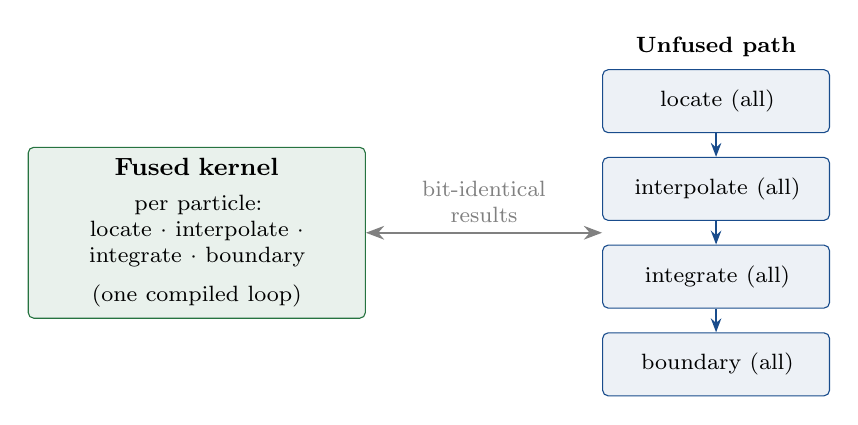
\begin{tikzpicture}[node distance=3mm and 7mm]
  \node[flowbox,text width=26mm] (u1) {\footnotesize locate (all)};
  \node[flowbox,below=of u1,text width=26mm] (u2) {\footnotesize interpolate (all)};
  \node[flowbox,below=of u2,text width=26mm] (u3) {\footnotesize integrate (all)};
  \node[flowbox,below=of u3,text width=26mm] (u4) {\footnotesize boundary (all)};
  \draw[flowarrow] (u1)--(u2); \draw[flowarrow] (u2)--(u3); \draw[flowarrow] (u3)--(u4);
  \node[font=\footnotesize,above=1pt of u1] {\textbf{Unfused path}};
  \node[flowbox,fill=laggreen!10,draw=laggreen,text width=40mm,minimum height=20mm,anchor=east]
    (F) at ($(u2.west)!0.5!(u3.west)+(-30mm,0)$)
    {\textbf{Fused kernel}\\[3pt]\footnotesize per particle:\\\footnotesize locate $\cdot$ interpolate $\cdot$\\\footnotesize integrate $\cdot$ boundary\\[3pt]\footnotesize (one compiled loop)};
  \draw[{Stealth[]}-{Stealth[]},gray,thick] (F.east) -- node[above,font=\footnotesize,align=center]{bit-identical\\results} (F.east -| u2.west);
\end{tikzpicture}
\caption{The two implementations of a single step. The fused kernel (left) performs all
per-particle operations inside one compiled loop; the unfused path (right) runs the same operations
as separate parallel passes over all particles. Where both exist they produce bit-identical
trajectories.}
\label{fig:fused}
\end{figure}

\section{Which path applies}\label{sec:fused-which}

\Cref{tab:fused-kernels} lists the fused kernel families and the conditions under which the step
functions choose them; every other configuration runs on the unfused path. In short: the
two-dimensional least-squares runs are fused for every integrator and every temporal treatment, except
Euler with \conf{em}/\conf{m1} diffusion (whose combined stochastic step replaces it) and, with the exact
guard off, HEALPix pixel meshes that fail the density certificate;
two-dimensional barycentric runs on node-layout velocities are fused when the flow is time-dependent,
reconstructed linearly and without element tracking;
three-dimensional runs are fused for Euler with least-squares velocities and for RK2 with node-layout
barycentric velocities on a z-level mesh. Among the paths that stay unfused are three-dimensional
RK4, every three-dimensional sigma-mesh run, element-layout barycentric and edge least-squares
interpolation, steady barycentric runs, and the \conf{idw} and \conf{leastsq} vertical combines of the
three-dimensional RK2 kernel. The last one matters in practice: the default
\conf{w\_interp: leastsq} keeps a node-layout three-dimensional RK2 run unfused, and setting
\conf{w\_interp} to \conf{nearest} or \conf{barycentric} moves it onto the fused kernel.

\begin{table}[t]
\centering\footnotesize\setlength{\tabcolsep}{4pt}
\begin{tabular}{@{}>{\raggedright\arraybackslash}p{30mm}>{\raggedright\arraybackslash}p{21mm}>{\raggedright\arraybackslash}p{73mm}@{}}
\toprule
kernel family & integrators & conditions \\
\midrule
2-D least squares, steady & Euler, RK2, RK4 & \conf{uv\_interp: leastsq} (element layout) \\
2-D least squares, time-aware & Euler, RK2, RK4 & as above; RK2 and RK4 with the next snapshot, Euler with a velocity between two snapshots, blended per element \\
2-D least squares, PCHIP & RK2, RK4 & as above, with \conf{temporal\_reconstruction: pchip} \\
2-D barycentric, time-aware & RK2, RK4 & \conf{uv\_interp: barycentric}, node layout, next snapshot present, linear in time, no carried element \\
3-D Euler & Euler & z-level mesh, \conf{uv\_interp: leastsq}, \conf{w\_interp} \conf{nearest} or \conf{leastsq} \\
3-D RK2 barycentric & RK2 & z-level mesh, node layout, \conf{uv\_interp: barycentric}, \conf{w\_interp} \conf{nearest} or \conf{barycentric}, no carried element; steady, linear or PCHIP \\
adaptive & RK45 & two-dimensional, element-layout least squares; this scheme has no unfused twin \\
\bottomrule
\end{tabular}
\caption{The fused kernel families and the configurations that select them. ``Carried element''
refers to \conf{elem\_search: walk} (\cref{sec:loc-walk}): the barycentric kernels keep their own
search, so a walk run takes the unfused path, while the least-squares kernels run and ignore the
carried element.}
\label{tab:fused-kernels}
\end{table}

The three-dimensional RK2 kernel evaluates per particle: the stage-one anchor and layer, the
horizontal velocity by barycentric interpolation with the temporal blend applied at each vertex, and
the vertical velocity $W_1$ --- computed before the horizontal verdict, so that a particle that dies
on the horizontal interpolation reports the same vertical velocity on both paths; the midpoint
$\mathbf{x}_{1/2}$ and $z_{1/2}=z+W_1\,\Delta t/2$; the stage-two anchor, layer and velocities; the end
position with $z_{\text{new}}=z+W_2\,\Delta t$; the containment test; and the clamp of the depth to the
water column. At one million particles on a mesh of \num{196000} nodes and 70 levels it was measured
1.30 times faster than the unfused path at 16 threads (a development measurement not kept in the
repository); the gain grows with the mesh and field size, while
scattered per-particle reads dominate both paths (\cref{sec:perf-schemes}). The two-dimensional
barycentric kernels remove the per-stage materialisation of the whole node field: on a
four-million-node mesh an RK4 step fell from \SI{83}{ms} to \SI{9}{ms} at eight threads, independent of
the mesh size.

\section{Bit-identity}\label{sec:fused-identity}

Where a fused and an unfused implementation of the same configuration both exist, they produce
bit-identical trajectories, statuses and failure reasons, which the test suite checks
(\cref{ch:validation}). Three things make it hold.

\paragraph{The temporal blend.} Rather than materialising the field at each stage time, the fused
kernels apply a nested two-level blend inline,
\begin{equation}\label{eq:fused-nested}
  \mathbf{u}_k=(1-\alpha_k)\bigl[(1-\alpha_0)\,\mathbf{u}_A+\alpha_0\,\mathbf{u}_B\bigr]+\alpha_k\,\mathbf{u}_T ,
\end{equation}
where $A$ and $B$ are the snapshots bracketing the step's start, $\alpha_0$ is the start's position in
that bracket, and $T$ is the stage \emph{target} snapshot the step moves toward --- the later bracket
snapshot when integrating forward, the earlier one when integrating backward, which is why the target
is passed separately from the bracket. \Cref{eq:fused-nested} performs the same floating-point
operations as stepping on the materialised field of \cref{eq:temp-linear}; with $\alpha_0=0$ it
collapses to a single blend, and the barycentric kernels short-circuit the end-point fractions exactly
as the unfused stage construction does, so the identity holds for non-finite values too.

\paragraph{The anchors.} Every evaluation site of a fused kernel --- the start, each stage and the
final position --- finds its nearest node through the exact search of \cref{sec:loc-exact}, the same
function the unfused batch query calls, so the two paths anchor every particle to the same node, ties
included. This is the default (\conf{mesh.exact\_nearest: true}). With the guard off, the fused
kernels widen an empty window ring by ring --- an approximate anchor --- and identity rests on gates
instead: the two-dimensional barycentric kernels (and the least-squares kernels on HEALPix pixel
meshes) run only on meshes that pass the density certificate of \cref{sec:loc-exact}, with a warning
and a fall-back to the unfused path otherwise; the three-dimensional RK2 kernel flags a particle whose
stage window is empty, repairs the flagged positions with the batch search and re-runs only those
particles through the kernel with the repaired anchor, for up to two rounds, before a last-resort
unfused re-run of the remainder. The least-squares kernels on FESOM-family meshes and the fused
three-dimensional Euler kernel have no such gate: with the guard off they agree with the unfused path
only where no three-by-three window is empty, which holds in the domain interior of quasi-uniform meshes.

\paragraph{The diagnostics.} Each fused kernel records why a particle failed --- interpolation failure
or out of bounds --- in a per-particle scratch array at its failure branches, and the caller merges it
into the sticky failure-reason field (\conf{mode.track\_failure\_reason}, \cref{ch:lifecycle}) exactly
as the unfused path does. A failed particle keeps its start position and anchor on both paths, and
frozen particles are copied verbatim.

\codeanchor{The fused kernels are the \fn{\_fused\_*} functions of \srcfile{numerics/integrators.py};
their runners are \fn{\_run\_fused\_2d}, \fn{\_run\_fused\_euler\_2d\_pair},
\fn{\_run\_fused\_2d\_tinterp}, \fn{\_run\_fused\_2d\_bary\_tinterp}, \fn{\_run\_fused\_2d\_pchip},
\fn{\_run\_fused\_euler\_3d} and \fn{\_run\_fused\_rk2\_3d\_bary\_tinterp}/\fn{\_pchip}; the adaptive
scheme is \fn{\_rk45\_kernel\_2d}. The dispatch lives in \fn{euler\_step}, \fn{rk2\_step} and
\fn{rk4\_step}; the anchor of each site is \fn{\_fused\_site\_anchor}; the guard-off gates are
\fn{\_bary\_fused\_anchor\_exact} and \fn{\_leastsq\_fused\_anchor\_exact}, and the repair loop
\fn{\_run\_fused\_3d\_with\_heal}; failure reasons are merged by \fn{\_merge\_fused\_failure}. The
unfused stage interpolation goes through \fn{\_interp\_uv\_at}. The inline blends are the
\fn{\_interp\_*\_tinterp} and \fn{\_interp\_*\_pchip4} cores of \srcfile{numerics/interpolate.py}
and, for the vertical velocity, of \srcfile{numerics/vertical.py}.}


\part{Stochastic Transport and Boundaries}
\chapter{Stochastic Diffusion}\label{ch:diffusion}

The resolved velocity field carries particles by advection, but it omits the mixing done by motions below
the model's resolution. The engine can represent this unresolved mixing as a random walk superimposed on
the advective step, turning the trajectory equation into a stochastic differential equation. This chapter
sets out the random-walk model and its treatment of the integration direction, how a horizontal kick moves
a particle on the sphere, the three horizontal schemes, the way the diffusivity and its gradient are
sampled from the mesh, the vertical random walk, the counter-based random-number generator that makes the
result reproducible and restart-safe, and how the kicks compose with the integrators. Diffusion is off by
default; when disabled it is byte-for-byte identical to a purely advective run.

\section{The random-walk model}\label{sec:diff-model}

A diffusivity $K_h$ spreads an ensemble of particles so that its variance grows linearly in time,
$\sigma^2 = 2K_h t$. The corresponding increment added to a particle over a step combines the
deterministic advective displacement with a random kick (\cref{fig:diffusion}):
\begin{equation}\label{eq:diff-step}
  \Delta x = u\,\dt \;+\; \xi\,\sqrt{2K_h\,\lvert\dt\rvert},
\end{equation}
where $\xi$ is a standard normal random variate drawn independently per component. With a spatially varying
diffusivity a drift term $\partial_x K_h\,\lvert\dt\rvert$ joins them (\cref{sec:diff-schemes}). The signs
follow three rules. The advective term carries the signed step, so it reverses under backward integration.
The random term uses $\sqrt{\lvert\dt\rvert}$ and spreads the ensemble in \emph{either} direction. The
drift uses $\lvert\dt\rvert$ too: it belongs to the diffusion, not to the advection, so a backward run
integrates the adjoint process, $-u+\nabla K_h$ plus the same noise. (A drift that reversed with the step
would leave a backward ensemble in a closed column with a stationary density proportional to $K^{-2}$
instead of a uniform one.) Diffusion is intrinsically irreversible; a backward run does not un-mix what a
forward run mixed, and the backward cloud is not a validated probability distribution of source positions.
The diffusivity may be anisotropic, with independent zonal and meridional components $K_x,K_y$.

\begin{figure}[t]
\centering
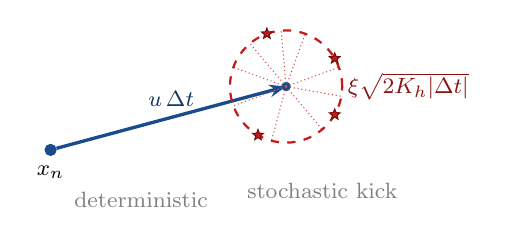
\begin{tikzpicture}[scale=1.15]
  \node[meshnode,label={[font=\footnotesize]below:$x_n$}] (A) at (0,0) {};
  \draw[-{Stealth[length=6pt]},lagblue,line width=1.2pt] (A)--(2.6,0.7) node[midway,above,font=\footnotesize,lagblue!70!black]{$u\,\dt$};
  \coordinate (B) at (2.6,0.7);
  \node[circle,fill=lagblue,inner sep=1.2pt] at (B) {};
  \foreach \a in {20,70,130,200,255,310,350,160,95}
     \draw[densely dotted,kelp!75] (B)--($(B)+(\a:0.62)$);
  \draw[dashed,kelp,line width=0.8pt] (B) circle (0.62);
  \node[font=\footnotesize,kelp!70!black] at (3.95,0.7) {$\xi\sqrt{2K_h|\dt|}$};
  \foreach \a in {30,110,240,330} \node[drifter,scale=0.5] at ($(B)+(\a:0.62)$) {};
  \node[font=\footnotesize,gray] at (1.0,-0.55) {deterministic};
  \node[font=\footnotesize,gray] at (3.0,-0.45) {stochastic kick};
\end{tikzpicture}
\caption{One diffusive step. The deterministic advective displacement $u\,\dt$ (blue) carries the particle
from $x_n$; a random kick of typical size $\sqrt{2K_h|\dt|}$ (dashed circle) is then added, scattering the
realized endpoint (stars). The advective term reverses under backward integration; the kick, scaling with
$\sqrt{|\dt|}$, spreads the ensemble either way.}
\label{fig:diffusion}
\end{figure}

\section{Kicks on the sphere}\label{sec:diff-sphere}

A kick is a displacement $(d_x,d_y)$ in metres, east and north. Added to longitude and latitude through the
metric of \cref{eq:int-displacement}, it would be a random walk on the longitude--latitude chart, which lacks
the drift $-K\tan\latx/R_M$ that a random walk on the sphere has: its particles would spread uniformly in
latitude rather than in area and would accumulate toward the poles. The engine therefore moves every
horizontal kick along the great circle. With $d=\sqrt{d_x^2+d_y^2}$, $\delta=d/R_M$ and the metric radius $R_M=\Mlat\cdot180/\pi$,
the position $\mathbf{r}=(\cos\latx\cos\lonx,\cos\latx\sin\lonx,\sin\latx)$ and the tangent displacement
\begin{equation}\label{eq:diff-tangent}
  \mathbf{t}=d_x\,(-\sin\lonx,\ \cos\lonx,\ 0)+d_y\,(-\sin\latx\cos\lonx,\ -\sin\latx\sin\lonx,\ \cos\latx),
\end{equation}
the kicked position is
\begin{equation}\label{eq:diff-expmap}
  \mathbf{r}'=\mathbf{r}\cos\delta+\frac{\mathbf{t}}{d}\sin\delta ,
\end{equation}
converted back to longitude and latitude. The east and north directions are taken at the stored longitude,
so the map is regular through a pole. For an anisotropic diffusivity the sphere adds one more term, a
northward drift $(K_x-K_y)\tan\latx\,\lvert\dt\rvert/R_M$ (with the latitude capped at $\pm89.9^\circ$); with
$K_x=K_y$ it vanishes and the uniform scheme is free of any drift.

\codeanchor{\fn{sphere\_displace}, \fn{sphere\_displace\_arrays} and \fn{anisotropic\_metric\_drift\_m} in
\srcfile{numerics/diffusion.py}.}

\section{The three horizontal schemes}\label{sec:diff-schemes}

The key \conf{diffusion.scheme} selects among three realizations of increasing fidelity to a spatially
varying diffusivity. The \conf{uniform} scheme uses a constant diffusivity taken from the configuration
(\conf{kh\_zonal}, \conf{kh\_meridional}) and adds the kick of \cref{eq:diff-step} with no gradient term.
The \conf{em} scheme (Euler--Maruyama) reads a spatially varying diffusivity from the dataset and adds the
Itô drift, per component,
\begin{equation}\label{eq:diff-em}
  \Delta x = u\,\dt+\partial_x K_x\,\lvert\dt\rvert + \sqrt{2K_x\lvert\dt\rvert}\;\xi_1 ,
\end{equation}
the drift being what prevents particles from accumulating spuriously in regions of low diffusivity and so
keeps the scheme consistent with the diffusion equation. The \conf{m1} scheme (Milstein) adds the next
term, $\tfrac12\partial_x K_x\,\lvert\dt\rvert\,(\xi_1^2-1)$; it is rigorous only for a separable diagonal
diffusivity and warns once whenever the field varies in space, for which \conf{em} is the safer
choice. With Euler (the combined composition) the diffusive part --- drift, Milstein term and noise ---
moves the particle along the great circle from the start of the step (\cref{sec:diff-sphere}) and the
advective part is added on the chart; with RK2 and RK4 (the split composition) the kick is applied at the
position the deterministic step reached. Where the diffusivity is constant, \conf{em} and \conf{m1} draw
the same normals as \conf{uniform}; only where the kick is applied differs.

\section{Sampling the diffusivity}\label{sec:diff-sampling}

The spatially varying schemes require both the diffusivity and its spatial gradient at the particle. The
diffusivity is read from node or element variables, their layout detected from the dimensions, and it must
not be negative. The value is obtained by the least-squares plane fit of \cref{sec:hvel-leastsq}, gated on
containment. The gradient is obtained by central differencing of that value over an offset
\conf{dres\_m} --- by default the median edge of up to \num{5000} sampled elements, clipped to
\SIrange{100}{50000}{\metre} --- with a fallback chain to a one-sided difference and then to the analytic
gradient of the fitted plane should the central difference be unavailable near a boundary.

\section{Vertical diffusion}\label{sec:diff-vertical}

In three dimensions on a z-level or sigma mesh, a vertical diffusivity $A_z$ adds a vertical random walk
(\conf{az\_enabled}, with a constant \conf{az\_const} or, on FESOM2 z-level output, a field \conf{var\_az}
on the interfaces). Its increment in positive-down depth is
\begin{equation}\label{eq:diff-az}
  \Delta\depx=\frac{\partial A_z}{\partial\depx}\,\lvert\dt\rvert+\sqrt{2A_z\lvert\dt\rvert}\;\xi ,
\end{equation}
with the drift mandatory: without it a walk in a non-uniform $A_z$ would collect particles where $A_z$ is
small \citep{visser1997random}. The field is taken from the nearest node's column, linear between
interfaces, with the depth clamped to the wet part of the column; the gradient is the slope of the same
linear segment --- on an interface, the segment above --- so that the value that sets the noise and the
gradient that sets the drift belong to one interpolant. A kick that leaves the column is reflected, not
clamped: with the column $[a,b]$, $L=b-a$ and $y=(\depx-a)\bmod 2L$, the new depth is $a+y$ for $y\le L$
and $a+2L-y$ otherwise, which handles any number of bounces. A clamp would pile particles up at the
boundaries; the reflection keeps a well-mixed column well mixed, which the tests check in a diffusivity
that varies tenfold over the column, in both directions of integration. The column is the surface to the
nearest node's floor on a z-level mesh and the particle's end-of-step column less $z_{0b}$ on a sigma mesh,
the same bounds as the depth clamp of \cref{sec:vert-clamp}. The vertical kick composes only with the
\conf{uniform} horizontal scheme, runs after the deterministic step and the horizontal kick, and with no
source configured the facility is dormant.

\codeanchor{\fn{diffusion\_az\_step\_meters}, \fn{az\_column\_value\_gradient}, \fn{reflect\_depth} and the
loops \fn{\_loop\_az\_kick\_zlevel} and \fn{\_loop\_az\_kick\_sigma} (\srcfile{numerics/diffusion.py});
applied by \fn{\_apply\_split\_az\_kick} (\srcfile{numerics/integrators.py}).}

\section{Reproducibility: counter-based random numbers}\label{sec:diff-rng}

The random kicks are generated not by a sequential pseudo-random stream but by a \emph{counter-based}
generator \citep{salmon2011philox}, in which each draw is a stateless hash of an integer key. The key is the
tuple of the configuration seed, the realization index, the \emph{original} particle index, the global step
index, and the component --- zero for the horizontal pair, one for the vertical kick --- from which a 64-bit
hash produces a uniform pair that is converted to a normal pair. Because each draw depends only on its key
and not on the order in which draws are issued, the result is bit-for-bit identical regardless of the
number of threads or the order of execution, and it is identical across a restart --- the same step index
regenerates the same kick. The particle index in the key must be the original, fixed index, not a
compacted index that shifts as particles die, or the stream would change when the live set changes. A run
over one shard of a larger release (\cref{sec:perf-shard}) adds the global index of its first particle,
\conf{data.particle\_offset} or the header that the splitting tool writes into each shard file, so a
particle draws the same numbers in the shard as in the unsharded run.

\section{Composition with the integrator}\label{sec:diff-composition}

How the stochastic kick combines with the deterministic step depends on the scheme and the integrator
(\conf{diffusion.composition}, resolved when the run starts). The \conf{uniform} scheme composes by
\emph{splitting}: the deterministic step (of any integrator, including RK45) is taken first and the kick
added afterward. The \conf{em} and \conf{m1} schemes with the Euler integrator \emph{combine}: the
stochastic differential equation replaces the Euler step as a whole; this mode needs element-layout
least-squares velocities. The same schemes with RK2 or RK4 use an opt-in split
(\conf{composition: split\_rk}), taking the Runge--Kutta step and then the kick, with the diffusivity
sampled at the start or, by default, at the end of the step (\conf{kh\_eval\_position}) and the kick applied
at the post-step position; the engine warns once that this is a pragmatic extension rather than a rigorous
scheme. The spatially varying schemes do not combine with RK45.

The kicked position is checked like any other: a kick that leaves the mesh returns the particle to its
position at the \emph{start} of the step with status \code{OUTSIDE}. In three dimensions only the
\conf{uniform}/split combination is available for the horizontal kick; the depth is clamped again at the
kicked position, and on a sigma mesh the particle keeps its fraction of the column. The combined and
split-with-Runge--Kutta modes raise an explicit error in three dimensions rather than apply an unvalidated
scheme. In time, the diffusivities are interpolated linearly with the velocity payload and are not included
in the monotone-cubic reconstruction.

\codeanchor{The schemes, the drift, and the Milstein term are \fn{diffusion\_uniform\_step\_meters},
\fn{diffusion\_em\_step\_meters} and \fn{diffusion\_m1\_step\_meters}; the counter-based generator --- a
keyed SplitMix64 hash in the counter-based spirit of \citet{salmon2011philox} --- and the Box--Muller pair
are in the same module, \srcfile{numerics/diffusion.py}. The composition is resolved by
\fn{\_resolve\_composition} (\srcfile{tracking.py}) and applied by \fn{\_apply\_split\_diffusion\_kick},
\fn{\_apply\_combined\_em\_step} and \fn{\_apply\_split\_rk\_em\_kick} (\srcfile{numerics/integrators.py});
the default offset is \fn{\_compute\_default\_dres\_m} (\srcfile{tracking.py}).}

\chapter{Particle Lifecycle and Boundary Conditions}\label{ch:lifecycle}

A particle is not simply a position that updates each step: it carries a status that records whether it is
being advected, has been removed, has stranded, or has not yet been released. This chapter describes the four
statuses and the transitions between them (\cref{fig:lifecycle}), the record of why a particle died, the
treatments of the domain's boundaries --- removal at the lateral boundary, clamping at the surface and floor,
and the optional periodic fold --- the optional beaching model, and the delayed-release mechanism by which
particles enter the simulation on a schedule.

\section{The four statuses}\label{sec:life-status}

Each particle holds one of four statuses. An \code{ALIVE} particle is advected normally and is the only kind
included in the working set that the integrator processes. An \code{OUTSIDE} particle has left the domain; the
status is terminal, and the particle is thereafter inert, its position frozen where it last was valid. A
\code{BEACHED} particle has stranded in shallow water; uniquely among the non-alive statuses it is reversible,
as a beached particle may refloat (\cref{sec:life-beach}). A \code{NOT\_RELEASED} particle has not yet reached
its scheduled release time; it is excluded from the working set, frozen in place at no computational cost,
until it is activated (\cref{sec:life-release}). Frozen positions are copied from step to step unchanged, not
re-wrapped, so a dead particle at longitude $180^\circ$ stays there.

\begin{figure}[t]
\centering
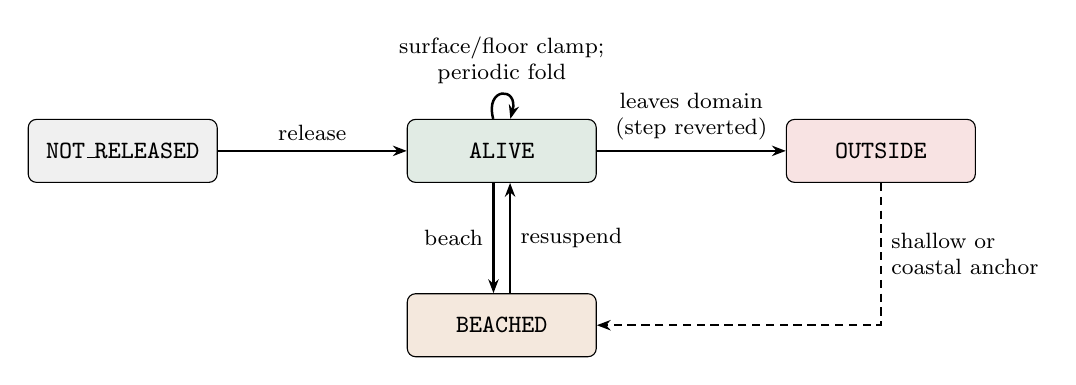
\begin{tikzpicture}[node distance=14mm and 24mm]
  \node[statebox,fill=gray!12] (NR) {\code{NOT\_RELEASED}};
  \node[statebox,fill=laggreen!14,right=of NR] (AL) {\code{ALIVE}};
  \node[statebox,fill=kelp!12,right=of AL] (OUT) {\code{OUTSIDE}};
  \node[statebox,fill=lagelem!14,below=of AL] (BE) {\code{BEACHED}};
  \draw[trans] (NR)--(AL) node[midway,above,font=\footnotesize]{release};
  \draw[trans] (AL)--(OUT) node[midway,above,font=\footnotesize,align=center]{leaves domain\\(step reverted)};
  \draw[trans,transform canvas={xshift=-3pt}] (AL)--(BE) node[midway,left,font=\footnotesize]{beach};
  \draw[trans,transform canvas={xshift=3pt}] (BE)--(AL) node[midway,right,font=\footnotesize]{resuspend};
  \draw[trans,densely dashed] (OUT) |- node[pos=0.25,right,font=\footnotesize,align=left]{shallow or\\coastal anchor} (BE);
  \draw[trans] (AL) edge[loop above,looseness=5] node[font=\footnotesize,above,align=center]{surface/floor clamp;\\periodic fold} (AL);
\end{tikzpicture}
\caption{The particle status state machine. A particle is released from \code{NOT\_RELEASED} into
\code{ALIVE} at its scheduled time; it is removed to \code{OUTSIDE} if it leaves the domain (its step undone).
With beaching enabled, \code{ALIVE} and \code{BEACHED} interconvert, and a particle removed in the same step
with a shallow or coastal anchor is reclassified as \code{BEACHED} (dashed). Reaching the surface or floor
does not change the status: the depth is clamped and the particle remains \code{ALIVE}; nor does a fold back
into a periodic window (the self-loop).}
\label{fig:lifecycle}
\end{figure}

\section{Why a particle died}\label{sec:life-reason}

With \conf{mode.track\_failure\_reason: true} each particle also carries a failure reason: none,
\emph{interpolation failed} (a stage found no fit or no containing element) or \emph{out of bounds} (the final
position lies in no element). Two further codes, for surface and bottom contact, are reserved and never set,
because those limits never remove a particle (\cref{sec:life-bc}). The reason is set once, when the particle
dies, and never overwritten; every integration path records it, fused and unfused alike (\cref{ch:fused}). A
beaching remap or a resuspension clears it, so the field keeps the meaning ``cause of death''. It is written
to the trajectory output and to checkpoints.

\section{Lateral removal versus vertical clamping}\label{sec:life-bc}

The engine treats the lateral boundary and the vertical limits in qualitatively different ways, and the
distinction is deliberate. The containing-element test of \cref{sec:loc-contain} is the lateral boundary
condition: a particle whose advected position is contained by no element has left the domain, and the engine
\emph{removes} it --- it sets the status to \code{OUTSIDE} and reverts the position to the start of the step,
so the particle does not record a spurious move across the boundary. A failed interpolation removes a particle
in the same way, and so does a diffusive kick that ends outside the mesh (\cref{sec:diff-composition}).
Because the test is geometric, an open boundary and a coastline are indistinguishable to it; both produce an
\code{OUTSIDE} result unless the beaching model says otherwise. The surface and the sea floor, by contrast,
are enforced by \emph{clamping} after the advective step (\cref{sec:vert-clamp}): a particle that would cross
either limit is held at it and continues to be advected. The vertical diffusive kick is the exception: it
\emph{reflects} at the limits, because a clamp would pile particles up there (\cref{sec:diff-vertical}).

\section{Periodic windows}\label{sec:life-periodic}

An idealized channel domain is made periodic in longitude, latitude or both by giving a window
$[x_0,x_1)$ in \conf{numerics.periodic\_lon} or \conf{numerics.periodic\_lat}. After every step, before the beaching hook and the
record, an alive particle outside the window is folded back,
\begin{equation}\label{eq:life-fold}
  x' = x_0 + \bigl((x-x_0)\bmod(x_1-x_0)\bigr),
\end{equation}
and receives a fresh nearest node; particles inside the window are left bit for bit untouched. Seeds are
folded once at the start, including those not yet released. The fold adds no connectivity across the seam, so
the mesh must extend beyond each periodic side by a \emph{ghost band} at least one step's displacement wide:
a particle must still be inside the mesh at the end of the step in which it crosses. The configuration is
checked before the output file is created: the windows must lie strictly inside $(-180^\circ,180^\circ)$ and
$(-90^\circ,90^\circ)$ and overlap the mesh, a periodic-longitude mesh must not straddle the $\pm180^\circ$
meridian, and a missing ghost band on either side produces a warning. Periodic windows cannot be combined with
a rotated frame (\cref{ch:frame}). The windows are written to the output metadata when set.

\section{Beaching and resuspension}\label{sec:life-beach}

When beaching is disabled (the default), every lateral exit becomes \code{OUTSIDE}. When the key
\conf{numerics.beaching.enabled} is set, a post-step hook strands particles by up to four criteria, combined
inclusively. The water column at the particle's nearest node is taken raw, $H=d+\eta$ when
\conf{use\_eta} is set and $H=d$ otherwise, without the minimum-thickness floor, which would hide tidal
drying; $\eta$ comes from the step's own velocity payload.
\begin{description}[font=\normalfont\conf,style=nextline,leftmargin=1.5em]
  \item[depth] $H<$ \conf{depth\_min}, or the node is marked dry by \conf{dry\_mask\_var}.
  \item[coastal\_element] the particle's containing element has an edge on the coast (an edge owned by one
    element only).
  \item[on\_failure] a particle the integrator has just removed is reclassified as \code{BEACHED} if its
    reverted anchor has $H$ below the zone depth or lies in a coastal element (the coastal test needs the
    coastal flags, built only when \conf{coastal\_element} or \conf{stochastic} is also a criterion); a removal in deep water at an
    open boundary stays \code{OUTSIDE}.
  \item[stochastic] within a near-shore zone --- $H<$ \conf{zone\_depth} (default twice \conf{depth\_min}), or
    coastal contact whenever the coastal flags exist --- a particle strands with probability
    $1-\exp(-\lvert\dt\rvert/t_{\text{beach}})$ per step.
\end{description}
A beached particle counts as re-wetted when $H>$ \conf{depth\_min} $+$ \conf{rewet\_hysteresis} and its node is
not marked dry; the hysteresis suppresses flicker between the two states. The resuspension policy is one of
\conf{never}; \conf{auto}, which refloats a particle after \conf{min\_wet\_steps} consecutive re-wetted steps;
\conf{stochastic}, which refloats a re-wetted particle with probability $1-\exp(-\lvert\dt\rvert/t_{\text{resuspend}})$;
and \conf{auto\_or\_stochastic}. The random draws use the counter-based generator of \cref{sec:diff-rng} with
their own components, keyed by the original particle index and the global step, and the count of re-wetted
steps is written to checkpoints, so a resumed run reproduces the uninterrupted one bit for bit.

The hook runs in two phases after the step: first the reclassification of just-removed particles, then the
criteria and the resuspension. Its containment test runs only for alive, beached and just-removed particles. The
coastal flags are built only when a criterion needs them. A configuration asking for $\eta$ without a
sea-surface height in the dataset, or naming a dry-mask variable that is absent, is refused at startup. On a
HEALPix mesh with neither a bathymetry variable nor \conf{mesh.levels} the node depths are zero, and the depth criterion would strand every particle.

\section{Delayed and pulsed release}\label{sec:life-release}

Release positions are read from the seed file. Two library helpers can write one: a regular grid over the
mesh extent, shrunk inward by a margin and filtered to points inside the mesh, and points scattered uniformly
in a circle of given radius around a centre, scaled by $\cos\latx$ so that the circle is round in metres.
Both work in the mesh's own coordinates: on a rotated mesh the caller rotates the centre into the mesh
frame and the kept points back to geographic before saving them as seeds.

Particles need not all enter at the start of the run. A per-particle release offset (a fourth column of the
seed file, in seconds from the start) and a pulse schedule that re-releases the whole seed set at a fixed
interval (\conf{time.n\_pulses}, \conf{time.pulse\_interval}) are both supported, and both are implemented by
pre-allocation and freezing rather than by growing the particle array. At setup the seed set is replicated to
its full final size --- the number of pulses times the number of seeds, pulse by pulse --- and each copy is given
a release step
\begin{equation}\label{eq:life-release}
  k_{\text{rel}}=\operatorname{round}\Bigl(\frac{t_{\text{rel}}+p\,\Delta t_{\text{pulse}}}{\dt}\Bigr)
\end{equation}
for pulse $p$, with a warning when the offset is not a whole number of steps. Particles whose release step
lies in the future begin as \code{NOT\_RELEASED}. At the top of each step the engine activates those whose
step has come, $k\ge k_{\text{rel}}$ in the global step count (so the rule holds for backward runs and across
restarts), flipping them to \code{ALIVE} so they are advected during that same step. A frozen particle costs
nothing in the kernel, which skips it, and the fixed array size is what allows the streaming output writer to
use a constant trajectory dimension. Dormant rows are written as missing values with their status; a particle
whose release step lies beyond the end of the run produces a warning and stays missing throughout. The output
records each particle's release position and release time, the start of the step in which it is activated
(\cref{eq:out-release}), so the rounded schedule can be read back from the file. The
diffusive noise is keyed by the global step, so a particle released later draws a different sequence from one
released at the start, by design. A run with a single release and no offsets reduces exactly to the
unscheduled case.

\codeanchor{The statuses and failure reasons are the enumerations \fn{ParticleStatus} and \fn{FailureReason} in
\srcfile{core/particles.py}; lateral removal and the revert are in the integrator kernels of
\srcfile{numerics/integrators.py}; the periodic fold and its checks are \fn{\_apply\_periodic\_wrap} and
\fn{\_validate\_periodic\_windows}, the beaching hook is \fn{\_apply\_beaching\_hook} (\srcfile{tracking.py})
over \fn{evaluate\_beaching} (\srcfile{numerics/beaching.py}); the release schedule is
\fn{build\_release\_state}, \fn{activate\_released} and \fn{mask\_dormant\_for\_record}
(\srcfile{core/release.py}).}


\part{Data, Configuration, and Validation}
\chapter{Forcing Input and Time Control}\label{ch:input}

The trajectories are driven by the model's stored velocity fields, which the engine reads on demand from disk
and places on a time axis. This chapter describes the reader layer and its lazy access to the forcing, the
requirement that the selected variables share a single time cadence --- the most common configuration error
on FESOM output --- the decoding of the time axis, the resolution of the integration window, the handling of
time-averaged forcing, the velocity handed to each step, and the cache through which several processes on a
node can share one copy of each snapshot. The in-memory read-ahead that serves the reconstruction of
\cref{ch:temporal} is part of this layer.

\section{The reader layer}\label{sec:input-reader}

A reader is selected by \conf{mesh.type}: \conf{fesom2}, \conf{fesom14}, \conf{fesomc}, \conf{nemo} or
\conf{healpix}. Each
provides the mesh, opens the forcing, and reads one snapshot at a time; the NEMO reader builds its mesh with
the engine's generic builder for structured grids, which turns the wet cell centres of a logically
rectangular grid into nodes and every four adjacent wet centres into a quadrilateral element. The forcing is opened \emph{lazily}: the dataset is mapped through \code{xarray}
without loading the field arrays, and a snapshot is materialized only when a step requires it.
\begin{description}[font=\normalfont\bfseries,style=nextline,leftmargin=1.5em]
  \item[FESOM2] The mesh comes from a mesh-diagnostics file (three naming conventions are recognised), an
    ASCII mesh directory or a Zarr store. For the multi-year layout --- one file per variable per year,
    \code{<var>.fesom.<year>.nc} --- the reader assembles exactly the variables the configuration names
    (velocities, surface height, sampled scalars, vertical diffusivity) and concatenates the years along time
    with \code{dask}, so a run may span decades without the files being merged on disk and naming
    \conf{unod} does not pull in fields that merely share a prefix. A directory in any other layout is
    assembled from the first matching file per velocity component and the other readable files on the mesh's
    dimensions.
  \item[FESOM~1.4] The mesh comes from the model's ASCII mesh directory or from the cell polygons of
    level-wise data (\cref{sec:mesh-fesom14}). The forcing, \conf{data.ncinput} (the files of
    \conf{ncinput\_v} and \conf{ncinput\_w} simply join it), is a file, a directory (its \code{*.nc} files in
    name order, hidden files skipped) or a glob pattern, for instance over the member directory of a CMIP6
    tree. Every file's header is read, and the files are grouped by the variables they hold, never by their
    names. Only the variables the run \emph{consumes} are opened: $u$ and $v$ (\conf{mode.var\_u},
    \conf{var\_v}, default \code{uo}, \code{vo}), in three dimensions $\Wvel$ (\code{wo}), the sea-surface
    height (\code{zos}) when a file holds it, every \conf{mode.sample\_vars} entry and, with beaching enabled,
    \conf{beaching.dry\_mask\_var}; a required variable that no file holds is refused, and the message lists
    what the files do hold. Two data forms are recognised from the dimensions: level-wise files
    $(\text{time},\text{depth},\text{node})$, such as the published CMIP6 output, and the raw writer's
    vectors over the three-dimensional nodes $(\text{time},\text{nodes\_3d})$, which are mapped onto the
    levels through the index table of the ASCII mesh. Model restart files, the mean files of an older model
    branch whose frame and time axis cannot be checked, and files whose layouts, levels or node coordinates
    disagree are refused. Every record of every variable is compared with the static wet mask of the mesh
    on every level before anything is changed; only then are $u$, $v$ and $\Wvel$ set to zero below the bed
    and sampled scalars continued downward from the column's last wet value, so that no fill value reaches a
    particle. The velocities come back on the levels, in node layout, with the placement \code{"level"}
    (\cref{sec:vert-uvdepth}); a two-dimensional run reads one level (\conf{mode.sigma\_layer}), the depth
    mean (\conf{mode.sigma\_mean}) or the surface. Without \code{zos} the surface height is zero. The
    reader resolves the time each record represents itself (\cref{sec:input-timeavg}). Refused before the
    output file exists: the \conf{em} and \conf{m1} diffusion schemes, since FESOM~1.4 output holds no
    diffusivity fields, and \conf{beaching.use\_eta} without a sea-surface height; the offline
    reconstruction of $\Wvel$ refuses FESOM~1.4 meshes, whose output holds \code{wo} itself.
  \item[FESOM-C] One NetCDF file carries the mesh and the forcing; separate files for $v$ and $w$ may be
    merged in.
  \item[HEALPix] The mesh is derived from the data store itself: its nodes are the wet pixel centres
    (\conf{mesh.healpix\_geometry: dual}, the default) or, with \conf{pixel}, the pixels are the elements
    and their corners the nodes (two-dimensional only); wet means finite velocity at the first record on
    the tracked level. Plain Zarr and NetCDF stores and
    reference stores (\code{.parq}, \code{.json}) are supported; the sea-surface height may come from a
    separate store with an identical time axis (\conf{data.ncinput\_eta}), and the vertical levels from
    \conf{mesh.levels} (\cref{sec:vert-coord}).
  \item[NEMO] The grid-T file is the input; the grid-U and grid-V files are found by substituting the grid
    token in its name and must share its time axis exactly. The first version is two-dimensional and requires
    a grid aligned with east and north.
\end{description}
A reader may also provide a hook \fn{prepare}, which checks the opened data against the mesh. It runs at every
entry: right after the data are opened, before any output file exists, and again at the entry of each
realization, after the \conf{max\_levels} cut, so it always sees the levels in use. The FESOM~1.4 hook only
checks --- the horizontal sizes, the full level axis, the node coordinates and the wet mask of the first record
of every variable --- and changes nothing. \code{kelp info} opens the data as a run does, the hook included.

Every reader that reads a vertical velocity converts it to the engine's positive-down convention
(\cref{sec:vert-wsign}; FESOM~1.4 writes \code{wo} positive up), and with \conf{velocity\_float32} stores the velocity fields in single precision to
halve their memory, the interpolation arithmetic staying in double precision.

\section{One cadence at a time}\label{sec:input-cadence}

FESOM output stores variables at several temporal cadences, set per variable in the model's configuration,
that nonetheless share a time-units string. The variables selected for a run must share a single cadence
(\cref{fig:cadence}): Lagrangian advection typically uses the daily node velocities and vertical velocity
together with the daily sea-surface height and any daily scalars, and must not mix them with monthly
element velocities. On the multi-year path the reader merges the selected variables onto a common time axis
with an exact join; a set that cannot be aligned raises an error with the hint that a mixed cadence is the
likely cause, the merged axis is checked to be strictly increasing, and a gap between years produces a
warning. On the other layouts every file attached to the velocity file (a separate $v$ or $w$, the
remaining files of a directory) is matched to the velocity records by time stamp: a file on another axis is
refused, and a finer one that contains every velocity stamp is thinned to them with a warning. A
mixed-cadence selection is easy to write and is caught only when the forcing is opened, not when the
configuration is read. The FESOM~1.4 reader applies the rule to the records it resolves: every consumed
variable must have exactly the records of $u$ (\cref{sec:input-timeavg}).

\begin{figure}[t]
\centering
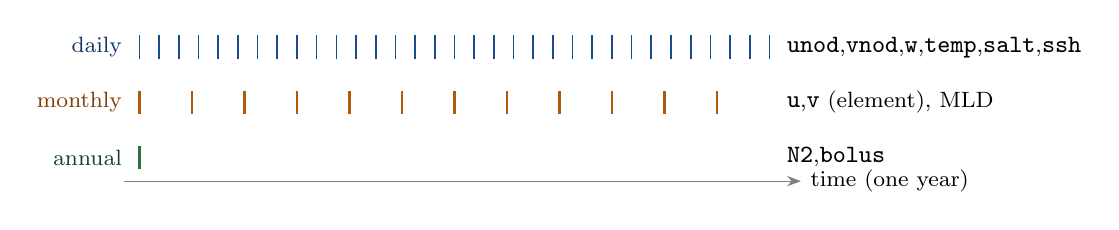
\begin{tikzpicture}[scale=1.0]
  \draw[-{Stealth[length=5pt]},gray] (-0.2,0)--(8.4,0) node[right,font=\footnotesize,black]{time (one year)};
  \foreach \x in {0,0.25,...,8.0} \draw[lagblue,line width=0.6pt] (\x,1.55)--(\x,1.85);
  \node[font=\footnotesize,left,lagblue!70!black] at (-0.1,1.7) {daily};
  \node[font=\footnotesize,right] at (8.1,1.7) {\code{unod},\code{vnod},\code{w},\code{temp},\code{salt},\code{ssh}};
  \foreach \x in {0,0.667,...,8.0} \draw[lagelem,line width=0.9pt] (\x,0.85)--(\x,1.15);
  \node[font=\footnotesize,left,lagelem!70!black] at (-0.1,1.0) {monthly};
  \node[font=\footnotesize,right] at (8.1,1.0) {\code{u},\code{v} (element), MLD};
  \draw[laggreen,line width=1.1pt] (0,0.15)--(0,0.45);
  \node[font=\footnotesize,left,laggreen!60!black] at (-0.1,0.3) {annual};
  \node[font=\footnotesize,right] at (8.1,0.3) {\code{N2},\code{bolus}};
\end{tikzpicture}
\caption{An example of the cadences of one FESOM2 output configuration: the variables share one time-units
string but are sampled at different rates. A run must select variables of a single cadence; Lagrangian
advection uses the daily node-based fields (top). Mixing cadences --- for example the daily
\code{unod}/\code{vnod} with the monthly element \code{u}/\code{v} --- cannot be aligned on one time axis and
is rejected when the forcing is opened (a finer attached file that contains every velocity stamp is thinned
with a warning instead).}
\label{fig:cadence}
\end{figure}

\section{The time axis}\label{sec:input-axis}

The snapshot times are converted to seconds from the first record. A datetime axis and a calendar-aware
(\code{cftime}) axis are converted directly; a numeric axis with units of the form ``\emph{unit} since
\emph{epoch}'' is decoded with its calendar; a numeric axis with a bare unit (days, hours, minutes, seconds
and their abbreviations) is scaled by that unit. An index axis $0,1,\dots,N-1$ without units is \emph{not}
taken as time; any other numeric axis without units is read as seconds. The snapshot spacing is the common difference when all differences agree to $10^{-3}$, and
\conf{numerics.dt} defaults to it. In the discrete mode \conf{numerics.dt} must equal that spacing, and an
irregular axis is refused; the interpolated mode accepts both. When the axis cannot be decoded, \conf{numerics.file\_dt} supplies the
spacing and the axis becomes $t_i=i\,\Delta t_{\text{file}}$; without either, the interpolated mode of
\cref{sec:temp-modes} is refused before the output file is created.

\section{The integration window}\label{sec:input-window}

The window in time is specified flexibly. The start is an index into the forcing record
(\conf{time.start\_time\_idx}) or a calendar date (\conf{time.start\_date}), parsed in the calendar of the
axis. In the interpolated mode the run starts at that instant, whether or not it coincides with a stored
time; in the discrete mode the date must coincide with a stored time, and the run starts at that record. The length is a number of integration
steps (\conf{time.n\_steps}, the preferred form), an explicit end index, or a duration in days
(\conf{time.duration\_days}, only together with \conf{time.start\_date}, converted to
$\lfloor\text{days}\cdot86400/\dt\rfloor$ steps). When the run reaches
the end of the available forcing it either stops or wraps to the beginning, according to
\conf{on\_exhausted}, the latter permitting a periodic forcing to be cycled. Multiple independent realizations
may be requested (\conf{num\_runs}), each offset in start time by \conf{run\_interval} snapshots, which is the
basis for ensembles with the stochastic schemes of \cref{ch:diffusion}; each realization writes its own output
file.

\section{Time-averaged forcing}\label{sec:input-timeavg}

Forcing is often stored as time averages --- daily or monthly means --- and the engine must know this to place
the snapshots correctly on the time axis. The key \conf{time\_averaging} declares whether the fields are
averages (\conf{mean}) or instantaneous samples (\conf{instant}). For averaged fields, whose file timestamps
conventionally mark the \emph{end} of each averaging window, the engine shifts each timestamp to the window
\emph{midpoint}, $\tilde t_i=(t_{i-1}+t_i)/2$ and $\tilde t_0=t_0-(t_1-t_0)/2$, before it is used for temporal
reconstruction, so that a daily-mean field is treated as representative of the middle of its day. Instantaneous
fields are used unshifted. We recommend setting this key explicitly: when it is omitted the engine warns and
guesses \conf{mean} for FESOM2 and HEALPix and \conf{instant} otherwise, and the guess, though usually correct,
is not guaranteed. A start date is matched against the \emph{unshifted} file times. In the interpolated mode
the run then starts at the named instant (until 2026-10-04 a date equal to a stored stamp started half a
window earlier, at the shifted midpoint, while a date one second later started on time); a date in the last
half window, past the last midpoint, starts at the last record with a warning. In the discrete mode the run
starts at the matched record.

\paragraph{Record times resolved by the reader (FESOM~1.4).} The FESOM~1.4 reader does not hand on the
stamps as written. It decodes every file with its own epoch and calendar --- the published CMIP6 files start a
new epoch every decade, raw output one per job segment --- and resolves, once per variable, the instant each
record represents: the \emph{centre of its averaging window} for a time mean, the stamp itself for a
snapshot. The window comes from exactly one source, in this order. First, the explicit keys
\conf{data.time\_stamp} (where a stamp sits in its window: \conf{start}, \conf{centre} or \conf{end}, or
\conf{instant} for snapshots) and \conf{data.time\_window} (\conf{calendar\_month}, \conf{calendar\_year},
\conf{calendar\_day} or a fixed duration such as \code{"5 d"}), given together; they decide for every file,
and when a file also has time bounds or an output schedule a warning names what was overridden and the
first record where the two disagree. Second, the files' time bounds, as in the CMIP6 files: a January record
bounded by 0 and 31 days represents day 15.5, that is, 12:00 on the 16th. Third, the raw writer's
\code{output\_schedule} attribute, whose stamps are the window ends in seconds since the job's start date; the
reader enumerates the output events the schedule implies and requires the stamps to be exactly those events.
Otherwise the run is refused with a message naming the two keys. The key \conf{data.time\_offset}
(\code{"<$\pm$number> <s|min|h|d>"}) is added to the stamps, the bounds and the epoch of every file before any
of this; it serves raw output of a job that started at a time of day other than midnight, whose stamps all sit
early by that time of day, and for raw-writer files it must lie in $[0,\SI{24}{\hour})$. Calendar windows are
computed exactly in the files' calendar, and with a calendar window a stamp that does not sit where
\conf{data.time\_stamp} puts it --- on a boundary of the window, or at its centre --- is refused. A window is never estimated from the spacing of neighbouring stamps, every record the source says must
exist has to be present --- a gap, a missing month or file, refuses the run --- and every consumed variable
must resolve to exactly the records of $u$, the same instants and windows to within \SI{1}{\milli\second}. The
last rule is the reader's form of the single-cadence requirement of \cref{sec:input-cadence}: the default raw
output, which writes \code{zos} daily and the velocities monthly, is refused, and the message suggests leaving
\code{zos} out of the input.

The resolved instants become the dataset's time axis, and nothing downstream moves them again. For this reader
the engine gives no warning, applies no midpoint shift, refuses a set \conf{data.time\_averaging}, and writes
\code{time\_averaging = "resolved\_by\_reader"} to the output. The refusal is deliberate: the shift of this
section assumes stamps at the window ends, whereas the reader's instants are already window centres --- a
CMIP6 monthly stamp, for instance, already sits in the middle of its month --- so a second shift would move
every record by half a window. Daily means therefore sit at 12:00, and a \conf{start\_date} is matched against
these centres: a discrete-mode start at midnight matches no record and needs \conf{temporal\_interp}. Monthly
means lie a calendar month apart, an irregular spacing that the discrete mode refuses, so they need the
interpolated mode. The three keys are refused for every other mesh type, and the run summary and
\code{kelp info} print one line saying what resolved the times, with the first and the last instant.

\codeanchor{\raggedright The record times are \fn{resolve\_axis} in \srcfile{readers/fesom14/\_timeaxis.py}, called per
consumed variable by \fn{Fesom14Reader.open\_dataset} (\srcfile{readers/fesom14/reader.py}); the keys reach it
through \fn{\_time\_option\_kwargs}, which also refuses \conf{data.time\_averaging} for the mesh types in
\code{\_READER\_RESOLVES\_TIME}, and \fn{\_describe\_record\_times} prints the summary line
(\srcfile{readers/\_\_init\_\_.py}); \fn{run\_tracking} (\srcfile{tracking.py}) skips the midpoint shift and
records \code{RESOLVED\_BY\_READER}.}


\section{The velocity handed to a step}\label{sec:input-payload}

Snapshots are read through a small cache keyed by record index, which keeps the bracketing pair, the PCHIP
stencil and the read-ahead window and releases the rest (\cref{sec:temp-prefetch}). Between two snapshots at
fraction $\interpfrac$ the step receives a lazy view of the pair rather than an interpolated field: each field
is blended, $(1-\interpfrac)\,a+\interpfrac\,b$, the first time a consumer reads it and is then cached, and a
field that no consumer reads is never blended --- the two-dimensional fused kernels and the
three-dimensional barycentric RK2 kernel read none, the fused three-dimensional Euler kernel reads the
blended velocities, and the beaching hook the surface height and a dry mask. At a snapshot, to within $10^{-12}$ in $\interpfrac$, the snapshot itself is passed. With the
view come the target snapshot and the time to it (\cref{sec:temp-linear}). Large blends run as a parallel
loop that is bit-identical to the array expression; fields stored in single precision are blended serially.

\codeanchor{The readers live in \srcfile{readers/} (one module per model; the registry and
\fn{extract\_time\_info} in \srcfile{readers/\_\_init\_\_.py}); the multi-year assembly and its cadence check
are in \srcfile{readers/fesom2.py}; the structured-grid builder is \srcfile{readers/structured.py}; the FESOM~1.4 reader is the package
\srcfile{readers/fesom14/} (\fn{Fesom14Reader} in \srcfile{reader.py}, the two data forms and the validity
predicate in \srcfile{\_layout.py}), and the \fn{prepare} hook is run by \fn{\_prepare\_dataset}
(\srcfile{readers/\_\_init\_\_.py}); the
midpoint shift (\fn{\_shift\_to\_midpoints}), the start date (\fn{\_resolve\_start\_date}), the payload
(\fn{\_build\_vel\_payload}) and the cache \fn{\_VelCache} are in \srcfile{tracking.py}; the lazy view
\fn{LazyLerpField} and its blend are in \srcfile{core/io.py}.}

\section{Sharing snapshots between processes}\label{sec:input-shared}

A large release is often split into several processes on one node (\cref{sec:perf-shard}), and each would
otherwise read and hold its own copy of every snapshot. With \conf{numerics.shared\_fields\_dir} set, one
process reads and publishes each processed snapshot and the others map the same bytes read-only
(\cref{fig:shared-cache}). A process that finds a snapshot missing takes a file lock; the one that wins
builds the arrays, writes them under a temporary name and renames the directory into place, which is atomic,
so a sibling never sees a partial snapshot. The writer keeps a window of three snapshots on either side of
the current one and removes the rest.

The snapshots live under a namespace derived from everything that determines their content: the
configuration keys that change what a snapshot read returns (mesh, mode, the input paths, the velocity
precision, the diffusivity and dry-mask variables), the size and modification time of the mesh and data files,
the engine version, and a \emph{generation}. The generation is the key
\conf{numerics.shared\_fields\_generation} when it is set; otherwise it is taken from the environment variable
\code{KELP\_SHARED\_FIELDS\_GENERATION}, and failing that from the batch job and job step. Shards of one job therefore
share a namespace, while another job, or a rewritten data file, never reuses a snapshot; without a generation
the run falls back to local reads. Each process registers itself on start and deregisters when it ends, and a
new cache removes namespaces whose processes have all ended. Every error of the shared layer falls back to
local reads with one warning, read-ahead is disabled, and the trajectories are identical with and without the
cache. Placed on the parallel file system and shared within one node, the cache costs almost nothing; shared
across nodes it slows every step (\cref{sec:perf-io}). Node-local memory (\code{/dev/shm}) has not been
measured.

\begin{figure}[t]
\centering
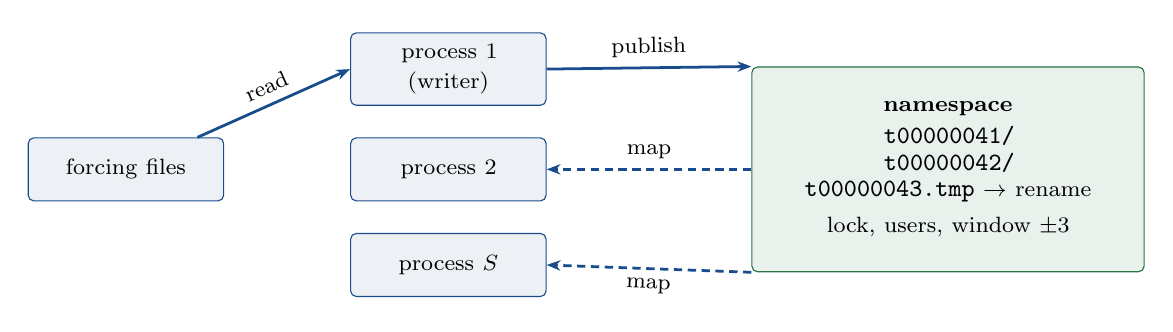
\begin{tikzpicture}[node distance=4mm and 8mm]
  \node[flowbox,text width=22mm] (p1) {\footnotesize process 1\\(writer)};
  \node[flowbox,text width=22mm,below=of p1] (p2) {\footnotesize process 2};
  \node[flowbox,text width=22mm,below=of p2] (p3) {\footnotesize process $S$};
  \node[flowbox,fill=laggreen!10,draw=laggreen,text width=47mm,right=26mm of p2,minimum height=26mm] (store)
    {\footnotesize\textbf{namespace}\\[2pt] \code{t00000041/}\\ \code{t00000042/}\\ \code{t00000043.tmp} $\to$ rename\\[2pt] lock, users, window $\pm3$};
  \node[flowbox,text width=22mm,left=16mm of p2] (data) {\footnotesize forcing files};
  \draw[flowarrow] (data)--(p1.west) node[midway,above,font=\footnotesize,sloped]{read};
  \draw[flowarrow] (p1.east)--(store.north west) node[midway,above,font=\footnotesize,sloped]{publish};
  \draw[flowarrow,densely dashed] (store.west)--(p2.east) node[midway,above,font=\footnotesize]{map};
  \draw[flowarrow,densely dashed] (store.south west)--(p3.east) node[midway,below,font=\footnotesize,sloped]{map};
\end{tikzpicture}
\caption{The node-shared snapshot cache. The process that wins the lock reads a snapshot from the forcing
files, writes it under a temporary name and renames it into place; the other processes map the published
arrays read-only. The namespace is derived from the configuration, the input files, the engine version and
the job, so no other run reuses it.}
\label{fig:shared-cache}
\end{figure}

\codeanchor{\fn{SharedFieldCache} in \srcfile{core/shared\_fields.py}; the namespace is
\fn{\_shared\_fields\_tag} with \fn{\_path\_fingerprint} and \fn{\_shared\_fields\_generation}
(\srcfile{tracking.py}).}

\chapter{Trajectory Output and Restart}\label{ch:output}

The product of a run is a set of trajectories: the recorded position, and any sampled properties, of every
particle through time. This chapter describes the two output backends and how to choose between them, the
variables written and their arrangement (output format~2, the format of release 1.0), the record time, the
provenance recorded with the trajectories, the checkpoint mechanism that allows a long run to be resumed and
continued in a chain of jobs, and the merging of a release split across processes. The authoritative
variable-by-variable description is \code{docs/io\_and\_time.md}, section~5.

\section{Two backends}\label{sec:out-backends}

The output format is chosen by the file extension of the output path. A \code{.zarr} path selects a chunked
Zarr store; any other selects a compressed NetCDF4 file (an unlimited record dimension, compression level 4).
The distinction is operationally significant for long runs. A NetCDF4 file is held under an exclusive write
lock for as long as it is open, so it cannot be inspected while the run proceeds; the key
\conf{output\_flush\_every} (command line \code{--flush-every}) mitigates this by buffering that many records
and then opening, appending, and closing the file, so that completed records become readable between flushes
and the file stays byte-identical. A Zarr store, by contrast, is lock-free and can be read while the run is
still writing. It buffers records in memory and writes one chunk of records at a time, so readers see it grow
in chunk-sized increments and a killed run loses at most one chunk of records; a checkpoint and the end of the
run flush the buffer. For multi-hour runs that one may wish to monitor, Zarr is the more convenient choice.

\paragraph{The Zarr layout.} Each variable is chunked in blocks of $n_t$ particles by $n_o$ records,
\begin{equation}\label{eq:out-chunks}
  n_t=\min(P,\ \num{500000}),\qquad
  n_o=\max\Bigl(1,\ \min\bigl(256,\ \bigl\lfloor 4\cdot10^{6}/(8\,n_t)\bigr\rfloor\bigr)\Bigr),
\end{equation}
so a chunk holds about \SI{4}{MB}. Up to half a million particles the particle axis is one block and a chunk
is one or more complete time columns; above that, a subset of particles reads only the blocks it touches.
Outputs written before this layout (August 2026) keep a single particle block.

\section{What is written}\label{sec:out-schema}

The output follows the CF conventions (the Climate and Forecast metadata conventions) for trajectories and
carries the global attribute \code{kelp\_output\_format} with the value~2; a file without it was written by an
earlier engine (\cref{sec:out-format1}). It is organized as a set of two-dimensional arrays indexed by
particle and by record, the \emph{trajectory} and \emph{time} dimensions (\cref{fig:output}), and both
dimensions have a coordinate variable of the same name. Every run writes the position --- longitude,
latitude and depth (positive down) --- the particle status as a coded flag (1 alive, 2 beached, 3 outside,
4 not released), the record time, a trajectory identifier, and, once per particle, the release position and
release time. The identifier is the particle's index in the whole release, so a shard of a sharded release
(\cref{sec:out-merge}) numbers its particles from its first global index. Several further variables are
written when they are present: the velocity as \code{vel\_u}, \code{vel\_v} and, in three dimensions only,
\code{vel\_w} (described below), the failure reason (\cref{sec:life-reason}), and one array per
sampled scalar field (\cref{ch:sampling}). Positions, release positions and horizontal velocities are always
written in geographic coordinates, un-rotated from any computational frame (\cref{ch:frame}). Where nothing
applies the arrays hold a fill value: a missing value (NaN) for positions, velocities, sampled fields and
release variables, and zero (no failure) for the failure reason; the rows of particles not yet released are
missing values. Positions carry the CF names and units (\code{longitude}, \code{latitude}, and
\code{depth} with \code{positive = "down"}), the status, failure reason and sampled fields name the
positions as their coordinates, and both backends write the same attributes. The one known departure from
CF is the order of the dimensions: CF wants the unlimited record dimension to be the outer one, while here
it is the inner one, so that the track of one particle is contiguous on disk.

A record is written after every step $g$ for which $g+1$ is a multiple of \conf{output\_freq}, counting steps
from the start of the run across any restarts. The release positions are therefore not part of the records ---
a particle first appears at the end of a step, at least one step after its release --- and are kept in the
separate release variables instead. The size of the output is proportional to
the number of particles times the number of records; for a large pulsed release this product, not the number
of live particles, sets the size, because the frozen particles occupy rows in the pre-allocated arrays. A run
with several realizations writes one file per realization, with the suffix \code{\_r}$N$.

\paragraph{The record time.} The time is stored in seconds since the first record of the forcing time axis
as it appears in the file, and the attributes of the time variable name that record's date as the epoch and
the forcing's calendar (for example \code{noleap} or \code{360\_day}), so that a reader such as xarray
decodes the values to dates. The record written after global step $g$ holds
\begin{equation}\label{eq:out-time}
  \tau_g=\tau_{\text{run}}+(g+1)\,\dt\,\tdir,
\end{equation}
the time at the \emph{end} of the step, in both time modes, where $\tau_{\text{run}}$ is the time at which
global step zero started. Let $g_{\text{s}}$ be the global index of the first step of the current call (zero for
a run that starts afresh). In the interpolated mode $\tau_{\text{run}}=t_{\text{first}}-g_{\text{s}}\,\dt\,\tdir$, with
$t_{\text{first}}$ the time at which the call's first step starts (the requested start date, or the time of the
start snapshot); in the discrete mode $\tau_{\text{run}}$ is the time of the snapshot $g_{\text{s}}$ records before
the call's start snapshot, the one the run started from. Under time-averaged forcing these
are the shifted midpoints (\cref{sec:input-timeavg}), so the dates are window centres, while the epoch stays
the first unshifted record. Because $\tau_g$ depends only on the global step and the start of the whole run,
the segments of a resumed chain carry exactly the labels of an uninterrupted run. In the discrete mode the
label advances by $\dt$ per step; the time-step check of \cref{sec:temp-modes} admits a small difference
between $\dt$ and the record spacing, by which the label may drift from the stored stamps. When the forcing is
cycled the time does not wrap: past the first period the dates lie beyond the end of the forcing, and an
attribute records the period. A forcing without a calendar epoch --- a bare unit, or an index axis with a
declared spacing --- gives plain seconds from its first record, with an attribute saying so.

\paragraph{Release positions and times.} For every particle the output holds its release longitude, latitude
and depth --- the seed position, after the fold into a periodic window when one is set --- and its release
time,
\begin{equation}\label{eq:out-release}
  \tau^{\text{rel}}=\tau_{\text{run}}+\max(k_{\text{rel}},0)\,\dt\,\tdir,
\end{equation}
the start of the step in which the particle is activated, with $k_{\text{rel}}$ the rounded release step of
\cref{eq:life-release} (zero without a delayed release). A particle never activated within the run still
gets its scheduled time, which then lies after the last record. The release positions travel with the
particle state and are stored in every checkpoint (\cref{sec:out-restart}), so each segment of a resumed chain
writes the same values; they are missing only for a run resumed from a checkpoint of an earlier engine.

\paragraph{Velocities.} The velocity of a record is the one the integrator evaluated for
the step that ends at the record, at the step's start position and time (for RK45, at its end); it therefore
names no coordinates. \code{vel\_w} is the rate of depth change, positive down, and on a sigma mesh the
dia-sigma flux (\cref{ch:vertical}). All components are flow velocities, with the same sign in forward and
backward runs (the integrators carry $\tdir$ times the velocity; the record removes the factor). A velocity is
written only where the particle was alive through the whole step --- alive after the release activation and
before the step, and alive after the step and the beaching hook. The record in which a particle dies or
strands, every later record of a beached or outside particle, a particle not yet released and a particle
resuspended during the step hold missing values. A two-dimensional run writes no \code{vel\_w}.

\begin{figure}[t]
\centering
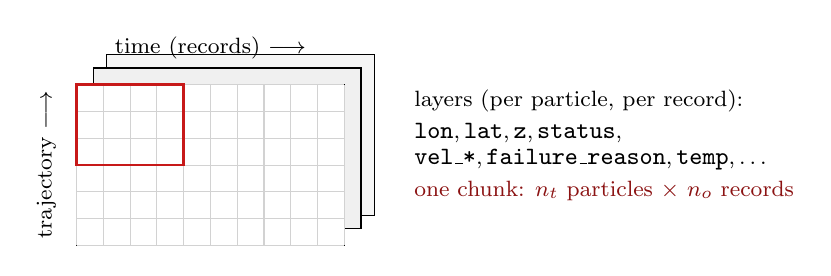
\begin{tikzpicture}[scale=0.85]
  \draw[fill=gray!8]  (0.45,0.45) rectangle (4.45,2.85);
  \draw[fill=gray!12] (0.25,0.25) rectangle (4.25,2.65);
  \draw[fill=white] (0,0) rectangle (4,2.4);
  \draw[step=0.4,gray!35,line width=0.4pt] (0,0) grid (4,2.4);
  \draw[kelp,line width=1pt] (0,1.2) rectangle (1.6,2.4);
  \node[font=\footnotesize,kelp!70!black,anchor=south west] at (0,2.4) {};
  \node[font=\footnotesize] at (2,2.95) {time (records) $\longrightarrow$};
  \node[font=\footnotesize,rotate=90] at (-0.45,1.2) {trajectory $\longrightarrow$};
  \node[font=\footnotesize,anchor=west,align=left] at (4.9,1.5)
    {layers (per particle, per record):\\[2pt]
     \code{lon},\,\code{lat},\,\code{z},\,\code{status},\\
     \code{vel\_*},\,\code{failure\_reason},\,\code{temp},\,\dots\\[2pt]
     \textcolor{kelp!70!black}{one chunk: $n_t$ particles $\times$ $n_o$ records}};
\end{tikzpicture}
\caption{The output data model: two-dimensional arrays indexed by particle (trajectory) and by record (time),
one such array per stored variable, with the time and the trajectory identifier as one-dimensional coordinate
variables and the release position and time as one-dimensional arrays over the particles. The position and
status are always present, and so are the velocities of a tracking run (NaN where none was evaluated);
failure reasons and sampled scalars are added when available. In a
Zarr store each array is split into chunks of \cref{eq:out-chunks}.}
\label{fig:output}
\end{figure}

\paragraph{Provenance.} Every output carries global attributes that record how it was produced: the
integrator, the step, the mesh type, the direction, the start index and step count, whether the run is
three-dimensional and time-interpolated, the temporal reconstruction and time averaging, the engine version,
the exact-anchor flag and the resolved grid-hash cell with the rule that chose it (\cref{sec:loc-cell}); in
three dimensions the vertical-velocity combine and sign convention. Options that are off by default add their
parameters only when they are on --- pulses, diffusion, beaching, the adaptive scheme's tolerance, periodic
windows, sampling, a non-default horizontal scheme or element search, single-precision fields, read-ahead and
the rotation angles --- so that an output written with the defaults carries none of them. A run is repeated
from these attributes; the recorded grid-hash cell, for instance, can be pinned to reproduce the anchors of
an earlier run.

\section{Checkpoints and restart}\label{sec:out-restart}

When \conf{checkpoint\_freq} is set, the engine writes a checkpoint after every step $g$ for which $g+1$ is a
multiple of it, overwriting the previous one, and a final checkpoint at the end, stamped with the last step
actually executed. The checkpoint lives in the output file itself as arrays named \code{restart\_*}: the
positions, statuses and nearest nodes, the release positions, the step and forcing indices, and --- when the
run uses them --- the failure reasons, release steps, carried elements, the counts of re-wetted steps and the
frame angles. Positions and release positions are stored in the computational frame. The arrays are created
by the first checkpoint, so an output written without checkpoints holds none of them. A flag,
\code{restart\_valid}, is created before any other checkpoint array and written as zero, cleared again before
every later checkpoint, and set only after all arrays are written; a checkpoint interrupted mid-write, the
first one included, is therefore detected rather than trusted. Checkpoints are off by default: a run killed
at a wall limit without them leaves nothing to resume from.

Resuming is done by the calling program rather than by a configuration key. It loads the checkpoint
(\fn{load\_restart}), checks its frame against the mesh, and continues with the next step index, the saved
counts of re-wetted steps and the forcing position; in the interpolated mode it also supplies the simulation
time, which the checkpoint does not store. For the record times of the continuation to equal those of the
uninterrupted run (\cref{eq:out-time}), the program passes the same forcing times as the first call ---
under time-averaged forcing the shifted midpoints --- and, when a cycled forcing is read in the discrete
mode, the start index counted on without wrapping (in the discrete mode the forcing index stored in the
checkpoint is that unwrapped index, so the index after it continues the run).
The release positions need no step of their own: they come back with the particle state. A program that
splits a resumed state into parts slices it with \fn{ParticleState.subset}, which slices every per-particle
array, the release positions included. With the exact-anchor guard the nearest nodes of the resumed state
are recomputed once.

\paragraph{Resumable chains.} A run longer than one allocation of a batch system is split into a chain of
jobs. Each job resumes from the newest standalone restart file --- written with \fn{write\_restart\_file}, which
writes the same arrays to a separate NetCDF file under a temporary name and moves it into place only after a
clean close, so a failed write keeps the previous restart --- writes its records into its own output segment,
and drops a numbered restart at every checkpoint (\cref{fig:out-chain}). At the end the segments are
concatenated along time. The concatenated chain equals one uninterrupted run bit for bit, because everything
that depends on time --- the random draws of diffusion and beaching, the release activation, the record and
checkpoint cadence --- is keyed to the global step index, never to the step within a job. The library supplies
these pieces; the driver that submits the chain belongs to the experiment.

\begin{figure}[t]
\centering
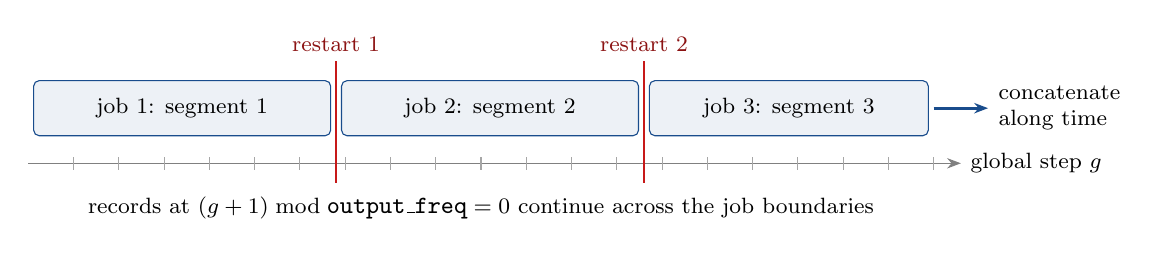
\begin{tikzpicture}[x=1.15cm,y=1cm]
  \draw[-{Stealth[length=5pt]},gray] (0,0)--(10.3,0) node[right,font=\footnotesize,black]{global step $g$};
  \foreach \j/\a/\b in {1/0/3.4,2/3.4/6.8,3/6.8/10.0}{
    \draw[flowbox,fill=lagblue!8] (\a+0.06,0.35) rectangle (\b-0.06,1.05);
    \node[font=\footnotesize] at ({(\a+\b)/2},0.7) {job \j: segment \j};
  }
  \foreach \x in {0.5,1.0,...,10.0} \draw[gray!70] (\x,-0.08)--(\x,0.08);
  \foreach \x/\lbl in {3.4/restart 1,6.8/restart 2}{
    \draw[kelp,line width=1pt] (\x,-0.25)--(\x,1.3);
    \node[font=\footnotesize,kelp!70!black,anchor=south] at (\x,1.3) {\lbl};
  }
  \node[font=\footnotesize,anchor=north,align=center] at (5,-0.3) {records at $(g+1)\bmod \text{\conf{output\_freq}}=0$ continue across the job boundaries};
  \draw[flowarrow] (10.0,0.7)--(10.6,0.7) node[right,font=\footnotesize,align=left]{concatenate\\along time};
\end{tikzpicture}
\caption{A resumable chain. Each job resumes from the newest numbered restart, writes its own segment and
drops restarts as it goes; the segments are concatenated at the end. Because every cadence and every random
draw is keyed to the global step, the result equals one uninterrupted run.}
\label{fig:out-chain}
\end{figure}

\section{Merging a sharded release}\label{sec:out-merge}

A large release split into contiguous blocks of seeds and run as parallel processes (\cref{sec:perf-shard})
produces one Zarr output per shard. The merge tool concatenates them along the trajectory axis in shard
order, after checking that the shards share their time axis, their variables and every attribute that
defines the run. A run with a single release merges into an output identical in its data to the unsharded run, stochastic
diffusion and beaching included, because each shard keys its random draws by the particle's index in the
full release; the merge refuses shards passed out of that order whenever the run draws random numbers (and
warns for a deterministic run). A pulsed release is refused. Shards that are independent by design --- a
pulsed run split through its restart, one seed per shard --- merge on an explicit option that lifts the offset
order, the pulsed refusal and the seed equality, refuses shards that share any seed of a random feature they
use over the same particle indices, and records each shard's particle count, offset and seeds in the merged store. Checkpoint
arrays are not merged. The merge keeps the time attributes and the release variables, and refuses shards that
differ in the output format, in the name of the record dimension, or in the units or calendar of the time;
shards of the earlier format merge as before.

\section{Outputs of earlier engines}\label{sec:out-format1}

Outputs written before release 1.0 are in output format~1. Such a file has no
\code{kelp\_output\_format} attribute, and its record dimension is called \code{obs}. In format~1 the record time has
no epoch: in the discrete mode it is the index of the snapshot the step started from, one step behind the
position it labels, and in the interpolated mode the seconds from the first record. Format~1 has no release
variables; a two-dimensional run writes a vertical velocity of zeros; a particle's velocity is written in the
record in which it dies or strands and is zero afterwards; the discrete mode samples scalar fields at the
start of the step; and the checkpoint arrays exist in every file, holding fill values when no checkpoint was
written. These files remain readable by \fn{load\_trajectories}, \fn{load\_restart}, the merge tool and the
visualization helpers; there is no converter.

% (plan Task 5 interfaces) on the final code.
\codeanchor{The writer \fn{TrajectoryWriter} and its NetCDF and Zarr backends, the embedded checkpoint,
\fn{write\_restart\_file}, \fn{load\_restart} and \fn{load\_trajectories} are in \srcfile{writers.py}; the record
cadence and checkpoint scheduling are in the time loop of \srcfile{tracking.py}, the record time and the release
variables in \fn{\_record\_clock\_origin} and \fn{\_release\_arrays} there; the epoch and calendar of the time
come from \fn{time\_axis\_epoch} (\srcfile{readers/\_\_init\_\_.py}); the velocity mask is
\fn{mask\_inactive\_velocity} (\srcfile{core/release.py}); the frame check on resume is
\fn{\_validate\_restart\_frame} (\srcfile{tracking.py}); sharding and merging are
\code{utils/sort\_seeds.py}, \code{utils/split\_seeds.py} and \code{utils/concat\_trajectories.py}.}

\chapter{Verification and Validation}\label{ch:validation}

The numerical methods of the preceding chapters are exercised by an automated test suite of about
\num{2450} tests, plus \num{18} slow ones that need external data and run separately. The large majority guard low-level invariants --- array shapes, configuration parsing,
byte-for-byte reproducibility --- and are not individually informative. This chapter does not enumerate
them. Instead it describes the tests that verify the numerical \emph{physics} against independent
references, organized by the kind of evidence they provide, and names each so that a reader may locate it.
The goal of these tests, and of this chapter, is to characterize whether the engine computes what it is
specified to compute, not to assess the physical realism of any simulation. Validation suites with pinned
tolerances are themselves tested: the code or the data is perturbed on purpose in a number of ways, and each
pin must fail; where a result has a natural ordering --- a finer resolution closer to the reference --- the
ordering is pinned as well.

\section{Closed-form analytic flows}\label{sec:val-analytic}

The most direct evidence comes from flows whose trajectories are known in closed form, for which the
computed path can be compared against the exact solution. The suite includes uniform flow, helical rotation
(with a test that the orbital radius is conserved), a Burgers vortex, inertial oscillations, an Ekman spiral,
and incompressible linear strain, whose exponential trajectory is matched to $2\cdot10^{-6}$ degrees
horizontally and \SI{8}{mm} vertically. Linear strain, solid-body rotation and downwelling are repeated on
quadrilateral meshes. In each case
the particle is integrated through the analytic field and its position checked against the formula, to
tolerances far below the grid scale. The edge least-squares scheme is checked to be exact for linear fields
inside triangles and quadrilaterals, to carry a flow parallel to a wall exactly under free slip, and to give
the same result on either side of the dateline. The adaptive scheme's coefficients are checked against the
Dormand--Prince order conditions, and its accuracy on a vortex against the tolerance and against RK4.

\section{Conservation and statistics}\label{sec:val-conservation}

A second class of tests checks conserved quantities and statistical laws that the numerics must respect.
For the three-dimensional vertical advection, the key tests exploit continuity: in a steady, divergence-free
flow a streamfunction exists and must be conserved along trajectories. Integrated through an analytic
downwelling cell, particles keep the streamfunction to 0.15\,\%; through an Ekman-pumping cell, to 3\,\% over
200 steps with the default vertical combine and 5\,\% over 100 steps with every combine. These are what verify
that the vertical-velocity interpolation neither creates nor destroys volume.

For the stochastic schemes, the ensemble variance is checked to grow as $\sigma^2=2K_h t$
(\cref{ch:diffusion}). On the sphere, the Monte-Carlo mean change of $\sin\latx$ under the horizontal kicks is
checked against the generator of the spherical random walk, $-2K_y\,h\sin\latx/R_M^2$ --- the walk on the
longitude--latitude chart gives half of it --- and particles are checked to cross a pole cleanly. In the
vertical, a uniform column in a diffusivity that varies tenfold must stay uniform: after \num{5000} steps each
of eight depth bins stays within 20\,\% of its share, forward and backward; without the drift term the density
would follow $1/A_z$ instead.

\section{Contracts with model data}\label{sec:val-data}

Some properties can only be checked against real model output; these tests run when the data are available
and are skipped otherwise. The sign of the vertical velocity (\cref{sec:vert-wsign}) is tested end to end ---
a file value of $+10^{-4}$\,m/s positive upward lifts a particle \SI{8.64}{\metre} in one Euler day --- and
against physics: in the equatorial Pacific at \SI{50}{\metre} the mean vertical velocity read from native
FESOM2 output, and from its HEALPix remap, must be upward. The HEALPix remaps are validated against the native
model: the same seeds run for thirty daily RK2 steps on the native mesh and on three HEALPix resolutions, and
the tests pin the ratio of median displacements, the median separation of paired trajectories, the mean
drift, the survivors, the ordering --- the finest remap closest to the native run --- and the equality of the
time axes, which catches a uniform one-day offset that the statistics alone would miss.

The sigma step of \cref{sec:vert-sigma-step} has exact solutions: with a tide, a sloping bottom, a horizontal
flow and a uniform dia-sigma velocity, the fraction of the column is linear in time, and Euler, RK2 and RK4
reproduce it to a relative $10^{-9}$, forward and backward, with uniform and stretched sigma levels; with a
dia-sigma velocity linear in the fraction the three schemes converge at orders one, two and four.

\begin{figure}[t]
\centering
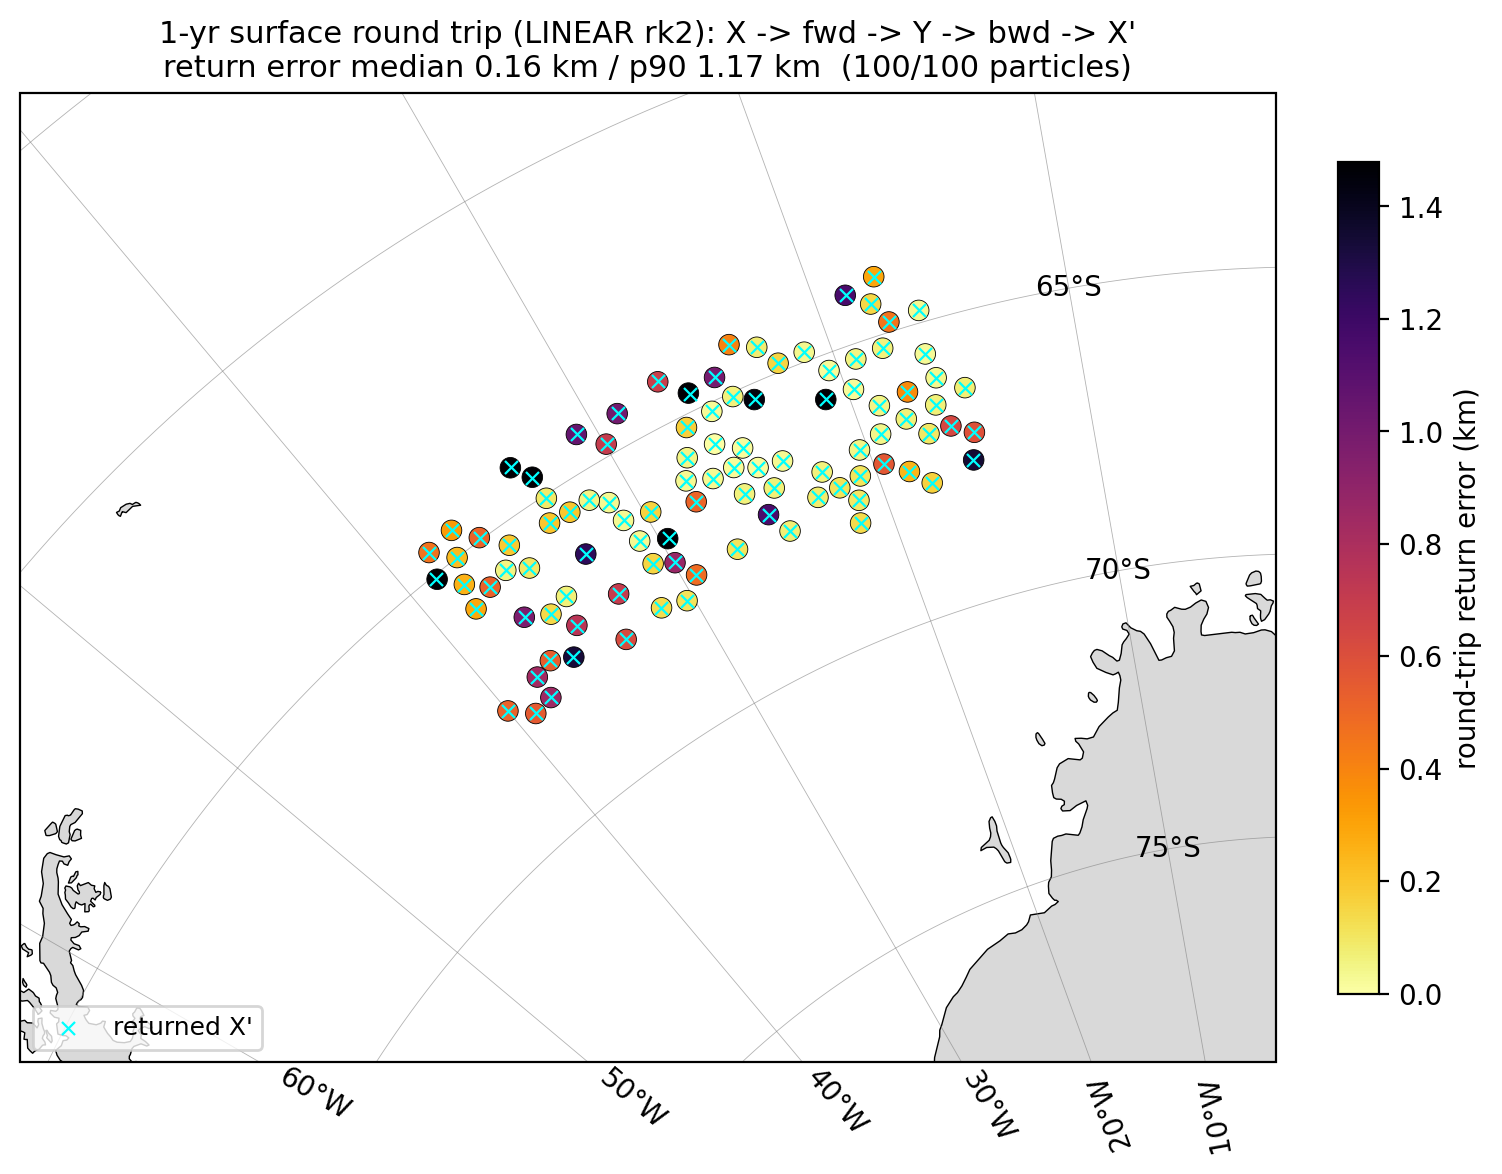
\includegraphics[width=0.72\linewidth]{revtest_roundtrip.png}
\caption{A controlled reversibility check on the \emph{core2} mesh, measured in June 2026: one hundred
particles are integrated forward for one year and then backward for one year with the same scheme (RK2,
linear reconstruction in time), and the return error between the start and end positions is mapped. The
median return error is \SI{0.16}{\kilo\metre} (ninetieth percentile \SI{1.17}{\kilo\metre}), far below the
local grid scale of tens of kilometres (a three-dimensional run at \SI{5}{\metre} depth in the Weddell Sea,
engine of June 2026; the vertical motion was negligible). Larger separations over long windows reflect Lagrangian chaos and
boundary clamping rather than a defect of the scheme.}
\label{fig:roundtrip}
\end{figure}

\section{Reversibility and determinism}\label{sec:val-reversibility}

A further class checks structural properties of the implementation. Because the deterministic integration
direction enters only as a sign on the velocity (\cref{sec:arch-direction}), a forward run followed by a
backward run should return a particle to its origin; the suite verifies this on analytic fields, including
under the monotone-cubic reconstruction, to $10^{-6}$ degrees in longitude, $10^{-9}$ in latitude and
\SI{1}{\micro\metre} in depth. The same property holds empirically on the \emph{core2} mesh: a clean one-year
surface round trip returns one hundred particles to a median of \SI{0.16}{\kilo\metre} (\cref{fig:roundtrip}).
With diffusion the backward run is the adjoint process, not the reversal of the forward one
(\cref{sec:diff-model}), and the tests check that the backward drift is kept.

Determinism is checked separately, as bit-for-bit identity. The fused and unfused kernels must agree for every
fused family, including the three-dimensional barycentric RK2 kernel and the monotone-cubic kernels
(\cref{ch:fused}); the exact nearest-node search must match a brute-force search on random geometries, and the
nearest-node kernels must match frozen copies of their earlier versions, ties included; element tracking must
give the same verdicts as the ring search. A resumed run must reproduce the uninterrupted one --- with
beaching, vertical diffusion, element tracking and sampling --- and must record the same steps; a checkpoint
interrupted mid-write must never load; a sharded release merged back must equal the unsharded run in its
data; and a run with the shared snapshot cache must equal one without it. The counter-based random numbers (\cref{sec:diff-rng}) are
independent of the thread count by construction: each draw depends only on its key.

\section{Time-dependent benchmark flows}\label{sec:val-benchmarks}

A constant zonal flow, a time-dependent moving eddy and a decaying eddy are integrated and compared with
their closed forms. A step-refinement test confirms the second-order ceiling
that linear-in-time reconstruction imposes on the whole scheme: halving the step cuts the RK4 error by a factor
between 3.5 and 5, not sixteen --- the $O(\Delta t^2)$ cap of \cref{ch:temporal} that the monotone-cubic
reconstruction lifts. Two diffusion benchmarks check the moments of Brownian motion and the skewness that a
spatially varying diffusivity must produce. These suites are marked slow and run outside the default test
run.

The engine adopts a metre-per-degree constant that differs from that of the original Fortran code, which
intentionally breaks bit-parity with it; the Fortran comparison is therefore not part of the suite, and the
Fortran prototype and its reference trajectories are not part of this repository.

\codeanchor{The physics-validation tests live in \srcfile{tests/}: the analytic-flow and streamfunction
families (\fn{test\_analytical\_3d\_benchmarks.py}, \fn{test\_downwelling\_psi.py}, \fn{test\_3d\_analytical.py},
\fn{test\_quad\_mesh\_benchmarks.py}); the random walks (\fn{test\_spherical\_random\_walk.py},
\fn{test\_az\_diffusion.py}); the data contracts (\fn{test\_w\_sign\_contract.py},
\fn{test\_healpix\_native\_twin.py}, \fn{test\_fesomc\_w\_contract.py}); the bit-identity pins
(\fn{test\_fused\_3d\_bary.py}, \fn{test\_exact\_nearest.py}, \fn{test\_node\_xyz.py}, \fn{test\_edge\_walk.py},
\fn{test\_checkpoint\_integrity.py}, \fn{test\_sharding.py}); and the reconstruction-order tests
(\fn{test\_temporal\_reconstruction.py}); the benchmark flows and diffusion benchmarks are the suites marked
slow.}

\chapter{Computational Cost and Performance}\label{ch:performance}

The cost of a run is governed by a small number of terms, and knowing them is what lets a study be
sized and configured sensibly. This chapter sets out the per-step budget, the per-particle cost of
the schemes and of the nearest-node search, how the work spreads over threads, processes and nodes,
what bounds memory, and how the cost is measured. Unless stated, the timings were taken on compute nodes
with two 64-core AMD EPYC 7763 processors (128 cores, \SI{256}{GB}), with the engine's own benchmark
scripts and verbose timing, and are collected in \srcfile{docs/performance.md}; the nearest-node rows
(the node coordinate table and \cref{tab:perf-guard}) were measured on a login node and are kept in
\srcfile{benchmarks/nearest\_scan\_table.md}. Absolute
values depend on the hardware and the mesh; the structure of the budget does not.

\section{The per-step budget}\label{sec:perf-model}

A step consists of four phases, and \code{kelp run --verbose} prints each of them for every step
(\code{io=}, \code{step=}, \code{beach=} when beaching is enabled, \code{rec=}) together with their
means at the end of the run:
\begin{equation}\label{eq:perf-model}
  t_{\text{step}} \approx t_{\text{read}} + t_{\text{blend}} + N\,c_{\text{kernel}} + t_{\text{record}},
\end{equation}
with $N$ the number of live particles. The \emph{read} term loads the snapshots the step needs; it
is set by the size of the field and by how often a new snapshot is needed, and it is independent of
the particle count and of where the particles are. The \emph{blend} term forms the velocity at the
step's time from the bracketing snapshots (\cref{ch:temporal}); it is paid only for the fields a
consumer actually reads, because the payload of a step blends a field on its first access and not
before. The \emph{kernel} term is the tracking itself --- locate, interpolate, advance --- and grows
with the number of live particles; dead and not-yet-released particles cost nothing. The
\emph{record} term writes a trajectory record every \conf{output\_freq} steps. The phases inside the
kernel are not separable in the fused kernels (\cref{ch:fused}); the verbose split is the finest
the engine reports.

Two consequences follow. A step that reads no snapshot and writes no record measures the kernel
alone; the \emph{steady step} of a run is therefore defined as the median, over the steps after
the first that read no snapshot, of the tracking phase --- and, for a run split over processes, of
the slowest process, which sets the completion time. And because the kernel cost of a step does not
depend on the time step, the cost of a model day grows linearly with the number of sub-steps per
snapshot interval: halving \conf{dt} doubles the run.

\begin{figure}[t]
\centering
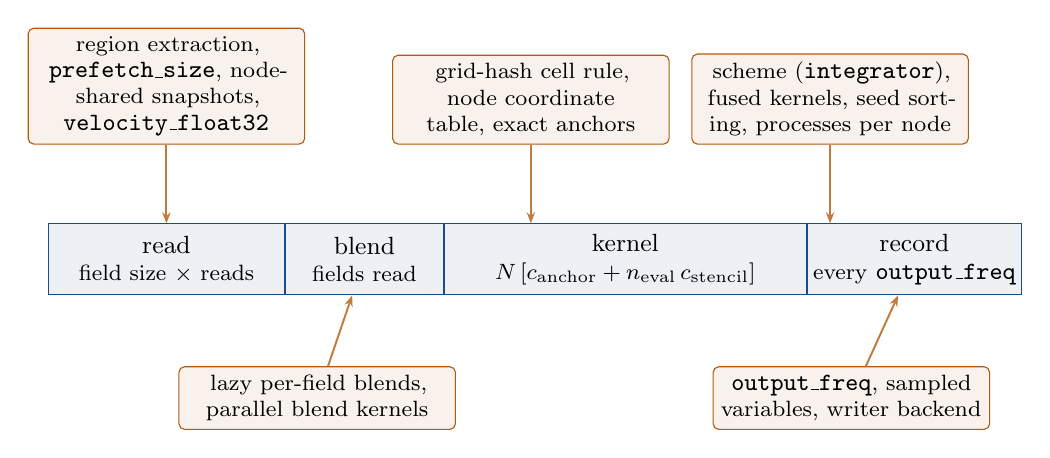
\begin{tikzpicture}[
  term/.style={rectangle,draw=lagblue,fill=lagblue!8,minimum height=9mm,align=center,font=\small,inner sep=2pt},
  lever/.style={rectangle,rounded corners=2pt,draw=lagelem,fill=lagelem!8,align=center,
                font=\footnotesize,text width=33mm,inner sep=3pt},
  lk/.style={-{Stealth[length=4pt]},line width=0.7pt,draw=lagelem!80}]
  \node[term,minimum width=30mm] (rd) at (0,0) {read\\[-1pt]\footnotesize field size $\times$ reads};
  \node[term,minimum width=20mm,right=0mm of rd] (bl) {blend\\[-1pt]\footnotesize fields read};
  \node[term,minimum width=46mm,right=0mm of bl] (kn) {kernel\\[-1pt]\footnotesize $N\,[c_{\text{anchor}} + n_{\text{eval}}\,c_{\text{stencil}}]$};
  \node[term,minimum width=22mm,right=0mm of kn] (rc) {record\\[-1pt]\footnotesize every \conf{output\_freq}};
  \node[lever,above=10mm of rd] (l1) {region extraction, \conf{prefetch\_size}, node-shared snapshots, \conf{velocity\_float32}};
  \node[lever,above=10mm of kn,xshift=-12mm] (l2) {grid-hash cell rule, node coordinate table, exact anchors};
  \node[lever,above=10mm of kn,xshift=26mm] (l3) {scheme (\conf{integrator}), fused kernels, seed sorting, processes per node};
  \node[lever,below=9mm of bl,xshift=-6mm] (l4) {lazy per-field blends, parallel blend kernels};
  \node[lever,below=9mm of rc,xshift=-8mm] (l5) {\conf{output\_freq}, sampled variables, writer backend};
  \draw[lk] (l1) -- (rd); \draw[lk] (l2) -- (kn.north -| l2); \draw[lk] (l3) -- (kn.north -| l3);
  \draw[lk] (l4) -- (bl); \draw[lk] (l5) -- (rc);
\end{tikzpicture}
\caption{The per-step budget of \cref{eq:perf-model} and the lever that acts on each term. The
kernel term splits into the nearest-node anchor ($c_{\text{anchor}}$, \cref{sec:perf-anchor}) and
the stencil work, repeated once per velocity evaluation of the scheme ($n_{\text{eval}}$).}
\label{fig:perf-budget}
\end{figure}

\section{The per-particle kernel cost}\label{sec:perf-schemes}

\paragraph{Schemes.} The kernel cost grows with the number of velocity evaluations per step. In two
dimensions, per particle and step at sixteen threads, forward Euler costs about \SI{1.1}{\micro s},
the midpoint method about \SI{6.6}{\micro s} and RK4 about \SI{22}{\micro s} (a June 2026
measurement, before the exact-anchor guard and the node coordinate table of
\cref{sec:perf-anchor}; the ladder, not the absolute values, is the point). The monotone-cubic
temporal reconstruction is blended inside the two-dimensional least-squares kernels and adds only a small fixed
offset, so the midpoint method with PCHIP is the cost-effective way to buy temporal accuracy
(\cref{ch:temporal}).

\paragraph{Three dimensions.} The fused three-dimensional midpoint kernel for node-layout
barycentric velocities on z-level meshes (\cref{ch:fused}) evaluates the whole step, including the
four-snapshot PCHIP blend, per particle; on steady steps its cost per particle does not depend on the
mesh (\cref{sec:perf-mesh}). The unfused three-dimensional paths --- among them RK4, sigma meshes, and
\conf{w\_interp} other than nearest or barycentric --- blend whole fields per stage. Those blends
run in a parallel kernel over contiguous double-precision fields, and RK4 reconstructs its repeated
midpoint stage once: a four-snapshot PCHIP blend of a global field of \num{47} layers by
\num{244000} elements (an element velocity field of the \emph{core2} mesh) takes \SI{46}{ms} at eight threads instead of \SI{953}{ms} serially, and a full
RK4 stage set (u, v, w, surface) about \SI{275}{ms} at eight threads and \SI{136}{ms} at 32. The
whole-field reconstruction is therefore no longer a multi-second floor of three-dimensional PCHIP
runs.

\codeanchor{Parallel blends: \fn{\_pchip\_blend4\_flat} in
\srcfile{numerics/temporal\_reconstruct.py} and \fn{\_blend} in \srcfile{core/io.py}; the lazy
payload is \fn{LazyLerpField} in \srcfile{core/io.py}; the stage dedup is in
\fn{make\_stage\_vels\_recon}.}

\codenote{The parallel linear blend requires double-precision inputs: with
\conf{velocity\_float32} the linear time interpolation falls back to a serial blend (about
\SI{0.25}{s} instead of \SI{0.05}{s} per global-size field), and the fused three-dimensional step
pays 15--20\,\% for the conversion on gather. The PCHIP blend converts first and keeps its parallel
path. Single precision is a memory lever, not a speed lever.}

\paragraph{The depth-linear rule.} Reading the horizontal velocity linearly in depth
(\cref{sec:vert-uvdepth}) costs two data points per stencil member instead of one, a search of the member's
column for the bracket and a test of the member against its bed. \Cref{tab:perf-depth-linear} gives what
this adds to one three-dimensional step, timed with the same arrays read in layer and in linear mode on
the compute node above (128 threads, \num{100000} particles at random positions, a synthetic HEALPix dual
mesh of \num{49152} nodes or its triangulated twin of \num{98300} elements, 21 layers down to
\SI{4000}{\metre} with varied bathymetry, a six-hour step; the median of fifteen interleaved steps per mode,
measured in October 2026). With a linear blend in time the rule adds about 10\,\% to the fused node-layout
RK2 step, 6\,\% to the fused element-layout Euler step and 3\,\% to the unfused element-layout RK2 step; with
the four-snapshot PCHIP blend the difference lies within the run-to-run spread, presumably because the
time blend then dominates the work per member. On a sigma mesh, where every step is unfused, the rule in the sigma
fraction costs between nothing measurable and 4\,\%. In the element workload about 16\,\% of the particles had
a dry element in their least-squares ring and about 4\,\% fewer than three wet ones, so the walls and the
area-mean fallback were exercised. Reading the records and the once-per-record check are not included.

\begin{table}[t]
\centering\footnotesize\setlength{\tabcolsep}{4pt}
\begin{tabular}{@{}llrrr@{}}
\toprule
step & time blend & layer [ms] & linear [ms] & ratio \\
\midrule
node layout, barycentric, fused RK2 & linear & 9.59 & 10.52 & 1.10 \\
 & PCHIP & 12.51 & 12.45 & 1.00 \\
element layout, least squares, fused Euler & linear & 7.30 & 7.75 & 1.06 \\
element layout, least squares, unfused RK2 & linear & 24.18 & 24.79 & 1.03 \\
 & PCHIP & 37.21 & 36.18 & 0.97 \\
sigma, element least squares, unfused RK2 & linear & 32.54 & 31.92 & 0.98 \\
 & PCHIP & 36.57 & 37.69 & 1.03 \\
sigma, node barycentric, unfused RK2 & linear & 36.51 & 37.51 & 1.03 \\
 & PCHIP & 34.49 & 35.71 & 1.04 \\
\bottomrule
\end{tabular}
\caption{Cost of the depth-linear rule per three-dimensional step: median milliseconds per step in layer
and in linear mode and their ratio, with the walls at depth of \cref{sec:vert-uvdepth}; \num{100000}
particles, 128 threads, two AMD EPYC 7763 processors. The Euler step reads its start field only and has no
PCHIP row.}
\label{tab:perf-depth-linear}
\end{table}

\codeanchor{\raggedright \srcfile{benchmarks/single\_node/depth\_linear\_cost.py} and its rows in
\srcfile{benchmarks/single\_node/depth\_linear\_cost.md}; the kernels compared are
\fn{\_fused\_rk2\_step\_3d\_bary\_tinterp} and \fn{\_fused\_rk2\_step\_3d\_bary\_pchip} against their
\code{\_dl} twins, \fn{\_fused\_euler\_step\_3d} against \fn{\_fused\_euler\_step\_3d\_dl}, and
\fn{\_rk2\_step\_unfused} with the layer and the depth-linear interpolation cores.}

\section{The nearest-node anchor}\label{sec:perf-anchor}

Every evaluation site starts from the nearest mesh node (\cref{sec:loc-nearest}), found by scanning
the nodes of a $3\times3$ window of grid-hash cells. The scan is linear in the number of nodes in the
window, so its cost depends on how many nodes a cell holds, and under the exact-anchor guard
(\conf{mesh.exact\_nearest}, the default) on how often the window must be widened before the
nearest node is proven. Three measures keep this term small.

\paragraph{The cell is chosen by measurement.} The automatic cell of the reader is
$2\sqrt{A/N}$, with $A$ the bounding-box area of the mesh in square degrees, and at least \ang{0.05}. On a mesh whose resolution varies by orders of magnitude, a cell
sized for the coarse part holds thousands of nodes in the refined part. Since September 2026 every
run chooses the cell itself (\conf{mesh.grid\_hash\_cell\_rule: occupancy}): it samples up to
\num{200000} element centres, finds each one's exact nearest node once, and, for candidate cells
$\ell_{\text{legacy}}/\sqrt{2}^{\,k}$, evaluates a per-query cost estimate --- the nodes of the window
plus nine cells plus one certificate for a provable hit, the nodes and cells of the widened
rectangle and one certificate per widening otherwise. It leaves the reader's cell only when the best
eligible candidate (at most 20\,\% widened queries, at most \SI{128}{MB} of hash offsets) promises at
least a 2.75-fold gain. Quasi-uniform meshes keep the reader's cell (the predicted gain is about two,
which buys nothing measurable on a step); structure-resolving meshes take a smaller one: a coastal
FESOM-C mesh goes from \ang{0.058} to \ang{0.014} (search 1.7 times faster) and an 11.5-million-node
global mesh from \ang{0.145} to \ang{0.051} (1.7--2.6 times). An explicit
\conf{mesh.grid\_hash\_cell\_size} always wins; the chosen cell and the rule are written to the
output metadata.

\paragraph{The node coordinate table.} The scans read unit-sphere coordinates of the nodes from a
table filled once when the hash is built, instead of evaluating trigonometric functions per
candidate. The pure scan is 6.3 times faster (\SI{3.2}{\micro s} to \SI{0.5}{\micro s} per query on one
thread), a two-dimensional midpoint step phase about twice as fast, at 24 bytes per node and process;
the trajectories are bit-for-bit unchanged.

\paragraph{The cost of exact anchors.} \Cref{tab:perf-guard} gives the cost of the guard for
\num{400000} particles at eight threads. It is a few per cent on HEALPix meshes and on the fused
three-dimensional kernel, about 40\,\% on a structured mid-latitude mesh even with every anchor provable,
and grows where many windows must widen --- at high latitude, where a degree of longitude shrinks, and with
a cell well below the node spacing. In every case the fused kernel with exact anchors stays faster
than the unfused path.

\begin{table}[t]
\centering\small
\caption{Cost of exact nearest-node anchors: one fused step, \num{400000} particles, eight threads,
milliseconds, with the node coordinate table. ``Off'' is the approximate in-window anchor; ``unfused''
is the unfused path under the guard.}
\label{tab:perf-guard}
\begin{tabular}{@{}lrrr@{}}
\toprule
Configuration & off & on & unfused \\
\midrule
structured mid-latitude mesh, automatic cell, RK4 & 115 & 157 & 230 \\
structured mesh at \ang{80}--\ang{88}\,N, automatic cell, RK4 & 102 & 201 & 278 \\
same, cell three times below the node spacing & 81 & 371 & 455 \\
HEALPix, polar band \ang{89}--\ang{89.9}\,N, RK4 barycentric & 531 & 855 & 961 \\
HEALPix, global uniform seeds, RK4 barycentric & 554 & 541 & 1019 \\
HEALPix at \ang{80}--\ang{88}\,N, fused 3-D midpoint barycentric & 398 & 385 & 406 \\
\bottomrule
\end{tabular}
\end{table}

\codeanchor{Cell rule: \fn{choose\_grid\_hash\_cell}, \fn{apply\_grid\_hash\_cell\_rule} and the
estimate \fn{\_gh\_sample\_stats}; table: \fn{\_node\_xyz\_fill}; exact search:
\fn{\_grid\_hash\_nearest\_exact}; all in \srcfile{core/mesh.py}. Benchmarks:
\srcfile{benchmarks/exact\_nearest\_cost.py}, \srcfile{benchmarks/nearest\_scan\_table.md},
\srcfile{benchmarks/grid\_hash\_cell\_rule\_table.md}.}

\section{Threads and processes on one node}\label{sec:perf-threads}

The kernels parallelize over particles. Two-dimensional fused kernels with single-precision
velocities scale steeply, about 38-fold for the midpoint method from one to 128 threads on a global
mesh. The fused three-dimensional midpoint kernel is not memory-bound: it gains 6.2-fold from 16 to
128 threads. The unfused three-dimensional paths are bound by memory bandwidth and saturate at 16 to
32 threads. The thread count must always be set explicitly (\code{NUMBA\_NUM\_THREADS}); left
unset, the kernel library occupies every logical core and small kernels slow down markedly.

A node can also be split into several processes, each tracking a contiguous share of the
particles and pinned to its own NUMA domain. \Cref{tab:perf-layouts} shows the effect for six million
particles in three dimensions on a zoom-9 HEALPix mesh with node-shared snapshots: the same 128 cores
take a 22\,\% shorter step as sixteen processes of eight threads than as one process of 128 (29\,\% more
particle-steps per second).

\begin{table}[t]
\centering\small
\caption{Process layouts on one node: 6.0 million particles, fused three-dimensional midpoint
barycentric kernel, zoom-9 HEALPix mesh (2.2 million wet surface nodes), 128 threads in total,
node-shared snapshots. Steady tracking step of the slowest process.}
\label{tab:perf-layouts}
\begin{tabular}{@{}lccccc@{}}
\toprule
Processes $\times$ threads & $1\times128$ & $2\times64$ & $4\times32$ & $8\times16$ & $16\times8$ \\
\midrule
Tracking step (s) & 0.576 & 0.540 & 0.489 & 0.478 & 0.447 \\
Throughput ($10^6$ particle-steps/s) & 10.4 & 11.1 & 12.3 & 12.6 & 13.4 \\
\bottomrule
\end{tabular}
\end{table}

\section{Mesh size and particle count}\label{sec:perf-mesh}

The kernel does not see the size of the mesh: a particle's work is a constant-size stencil around
its position. \Cref{tab:perf-mesh} confirms this for the fused three-dimensional step over a
3765-fold range of HEALPix meshes with the same six million particles --- the step varies by at most
1.45 times, and not monotonically; the search window holds a median of 57--65 nodes on all seven
meshes, so the variation is not the nearest-node search. The step grows slightly less than linearly
with the number of particles (\cref{fig:perf-particles}): from \SI{0.144}{\micro s} per particle-step at
three million to \SI{0.106}{\micro s} at 24 million on 128 threads, a log--log slope of 0.88.

\begin{table}[t]
\centering\small
\caption{Mesh size: 6.0 million particles, one 128-thread process, fused three-dimensional midpoint
barycentric kernel, HEALPix meshes of zoom 5 to 11.}
\label{tab:perf-mesh}
\begin{tabular}{@{}lrrrrrrr@{}}
\toprule
Zoom & 5 & 6 & 7 & 8 & 9 & 10 & 11 \\
\midrule
Wet surface nodes ($10^6$) & 0.009 & 0.036 & 0.14 & 0.57 & 2.2 & 8.9 & 35.5 \\
Tracking step (s) & 0.742 & 0.814 & 0.628 & 0.803 & 0.638 & 0.635 & 0.908 \\
\bottomrule
\end{tabular}
\end{table}

\begin{figure}[t]
\centering
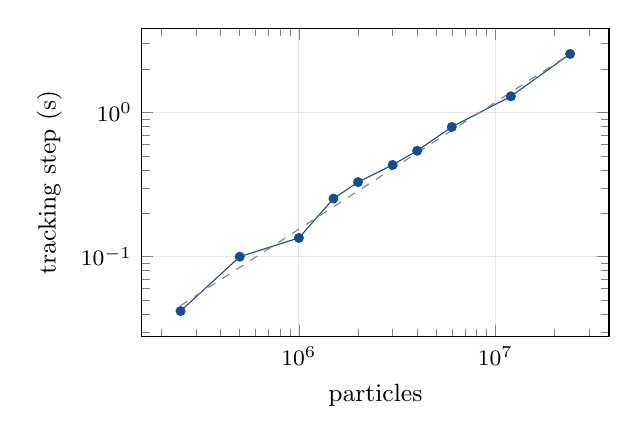
\begin{tikzpicture}
\begin{loglogaxis}[width=0.62\linewidth,height=55mm,xlabel={particles},ylabel={tracking step (s)},
  grid=major,grid style={gray!20},tick label style={font=\footnotesize},label style={font=\small}]
\addplot[mark=*,color=lagblue,mark size=1.6pt] coordinates {
  (0.25e6,0.042) (0.5e6,0.100) (1.0e6,0.135) (1.5e6,0.253) (2.0e6,0.329) (3.0e6,0.433)
  (4.0e6,0.543) (6.0e6,0.794) (12e6,1.295) (24e6,2.546)};
\addplot[dashed,color=gray,domain=0.25e6:24e6,samples=2] {0.106e-6*x*(24e6/x)^(0.12)};
\end{loglogaxis}
\end{tikzpicture}
\caption{Particle count: steady tracking step against the number of particles, zoom-10 HEALPix mesh
(8.9 million wet surface nodes), one 128-thread process, fused three-dimensional midpoint kernel.
Dashed: the fitted power law with slope 0.88.}
\label{fig:perf-particles}
\end{figure}

\section{Many nodes}\label{sec:perf-nodes}

Particles are independent, so a release splits over nodes as contiguous shares, one or several
processes per node, each reading its own snapshots or sharing them within the node
(\cref{sec:perf-io}). \Cref{fig:perf-nodes} shows weak and strong scaling on the zoom-11 HEALPix mesh
(35.5 million wet surface nodes, 69 layers), one 128-thread process per node --- a zoom-11 process
needs about \SI{146}{GiB}, so one fits a \SI{256}{GB} node. With six million particles per node the
step stays within 90\,\% of the one-node value up to sixteen nodes (96 million particles in
\SI{0.85}{s}, $113\times10^{6}$ particle-steps per second). A fixed release of 24 million particles
runs 12.6 times faster on sixteen nodes; on the zoom-9 mesh, split as eight processes per node, six
million particles run 9.7 times faster on sixteen nodes, where each process holds only
\num{47000} particles.

Very large releases keep the same throughput. Tracked for a few steps without any output, $10^{9}$
particles on sixteen nodes step in \SI{7.6}{s} and $10^{10}$ particles on sixteen \SI{512}{GB} nodes in
\SI{73}{s} --- both about $1.3\times10^{8}$ particle-steps per second.

\begin{figure}[t]
\centering
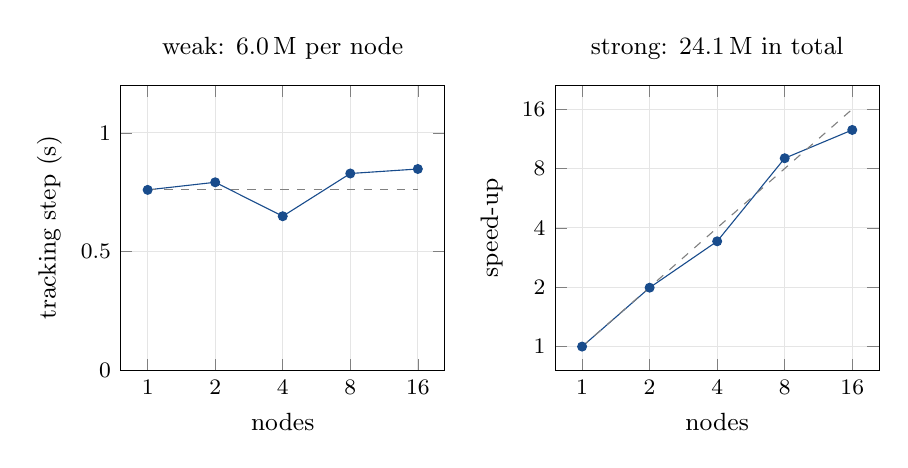
\begin{tikzpicture}
\begin{axis}[name=weak,width=0.47\linewidth,height=52mm,xmode=log,log basis x=2,
  xtick={1,2,4,8,16},xticklabels={1,2,4,8,16},xlabel={nodes},ylabel={tracking step (s)},
  ymin=0,ymax=1.2,grid=major,grid style={gray!20},title={weak: 6.0\,M per node},
  title style={font=\small},tick label style={font=\footnotesize},label style={font=\small}]
\addplot[mark=*,color=lagblue,mark size=1.6pt] coordinates {(1,0.760) (2,0.792) (4,0.649) (8,0.829) (16,0.848)};
\addplot[dashed,color=gray,domain=1:16,samples=2] {0.760};
\end{axis}
\begin{axis}[at={(weak.east)},anchor=west,xshift=14mm,width=0.47\linewidth,height=52mm,
  xmode=log,ymode=log,log basis x=2,log basis y=2,xtick={1,2,4,8,16},xticklabels={1,2,4,8,16},
  ytick={1,2,4,8,16},yticklabels={1,2,4,8,16},xlabel={nodes},ylabel={speed-up},
  grid=major,grid style={gray!20},title={strong: 24.1\,M in total},title style={font=\small},
  tick label style={font=\footnotesize},label style={font=\small}]
\addplot[mark=*,color=lagblue,mark size=1.6pt] coordinates {(1,1.00) (2,1.99) (4,3.42) (8,9.02) (16,12.55)};
\addplot[dashed,color=gray,domain=1:16,samples=2] {x};
\end{axis}
\end{tikzpicture}
\caption{Scaling over nodes on the zoom-11 HEALPix mesh, one 128-thread process per node, fused
three-dimensional midpoint kernel. Left: weak scaling (dashed, the one-node step). Right: strong
scaling of 24.1 million particles (dashed, ideal). The strong curve is not smooth because the cost of
a process depends on which particles its contiguous share holds.}
\label{fig:perf-nodes}
\end{figure}

\section{Memory}\label{sec:perf-memory}

A process holds the mesh, the node coordinate table (24 bytes per node), the hash offsets (at most
\SI{128}{MB} under the cell rule), the snapshots of the read window, and the particle state. For
releases large enough that the particles dominate, the peak resident memory of a
three-dimensional midpoint process without output was measured as
\begin{equation}\label{eq:perf-memory}
  M_{\text{peak}} \approx \SI{61}{GiB} + \SI{181}{B} \times N_{\text{process}}
  \qquad\text{(zoom-11 mesh, fused 3-D midpoint, no output)},
\end{equation}
fitted through one-node releases of $10^{9}$ (\SI{230}{GiB}) and $4\times10^{9}$ particles
(\SI{735}{GiB}); it predicted \SI{166.7}{GiB} for 625 million particles per process where
\SI{166.2}{GiB} was measured. Below about $4\times10^{8}$ particles per process the snapshot read,
not the particles, sets the peak (122--146 GiB on this mesh). A small probe therefore measures the
read, not the cost per particle; a new configuration is sized from two releases large enough for the
particles to dominate.

\section{Input and output}\label{sec:perf-io}

\paragraph{The read term dominates runs that write.} For a full model year of six million
three-dimensional particles on a zoom-9 mesh with daily snapshots and six-hour steps, one 128-thread
process took 2 hours 12 minutes: of the mean step of \SI{5.33}{s}, reading took \SI{2.94}{s},
tracking \SI{0.62}{s} and writing \SI{1.78}{s} (\SI{7.1}{s} per record, every fourth step). Input and
output make up 88\,\% of the step. On the zoom-11 mesh one daily snapshot costs about \SI{146}{s} per
process --- as much as some 190 tracking steps of six million particles.

\paragraph{Levers on the read term.} Confining a study to part of the ocean does not by itself
reduce the read on a global mesh; extracting the region into a smaller mesh and forcing once, before
the run, reduces the input volume by about two orders of magnitude and improves the thread scaling,
because the smaller field fits in cache. The read-ahead (\cref{sec:temp-prefetch}) amortizes the
per-read overhead; it is forced to one snapshot when snapshots are shared between processes or when
the forcing is cycled. Several processes on one node can share one copy of each processed snapshot
(\conf{numerics.shared\_fields\_dir}): one process, elected by a file lock, publishes each snapshot
with an atomic rename and the others map it read-only. Every measurement placed the cache on the
parallel file system: shared within one node it was nearly free and removed the per-process replication
(\SI{16}{GB} to \SI{10}{GB} per process in one layout); shared by several nodes it slowed every step,
because remote nodes fault pages in while stepping. Node-local memory has not been measured. The outputs are bit-for-bit identical with and without the shared
cache, and any failure of the shared layer falls back to local reads.

\paragraph{Output.} The volume grows with the number of particles and records: at most about \SI{66}{B} per
particle and record uncompressed (positions, status, velocity diagnostics and two sampled fields, the
velocity diagnostics some 40\,\%), and about \SI{37}{B} on disk in the one measured compressed store
(six million particles, one year); \conf{output\_freq} is the
lever, and sampled variables add their own columns. A pulsed release stores the whole pre-allocated
array at every record, released or not.

\codeanchor{Read window and shared snapshots: \fn{\_VelCache} in \srcfile{tracking.py},
\fn{SharedFieldCache} in \srcfile{core/shared\_fields.py}; region extraction:
\srcfile{utils/extract\_fesom\_region.py} and \srcfile{utils/extract\_healpix\_region.py}; sharding:
\srcfile{utils/sort\_seeds.py}, \srcfile{utils/split\_seeds.py}, \srcfile{utils/concat\_trajectories.py}.}

\section{Sharding a release}\label{sec:perf-shard}

A release is sharded in three steps: the seeds are sorted spatially (by HEALPix cell, then depth),
so that consecutive particles share cached velocity data --- worth 17\,\% on the fused
three-dimensional step at a million particles; the sorted file is split into contiguous shares, one
per process; and the per-process outputs are merged in shard order afterwards. A deterministic run
with a single release, sharded and merged, is data-identical to the unsharded run, stochastic features
included: the splitting tool writes each shard's position in the full release into the shard file, and
the engine keys every random draw by the particle's index in the full release (\cref{sec:diff-rng}).
All shards therefore use the same seeds.

\section{Measuring the cost}\label{sec:perf-measure}

Three measurements cover most questions. The verbose per-step phase split of
\cref{sec:perf-model} tells which term dominates a run; the steady step --- the median tracking
phase over read-free steps after the first, of the slowest process --- is the number to compare
between runs and configurations, never a mean that mixes steps that read snapshots with steps that
do not. The portable single-node benchmark (\srcfile{benchmarks/single\_node/run\_bench.py}) builds a
synthetic HEALPix store and reports the machine-independent \emph{thread-microseconds per
particle}, its steady step (the mean of its last five steps) times the thread count divided by the
particles: on the compute node
above 15.7--19.9 thread-\si{\micro s} from 16 to 128 threads, on a laptop's five performance cores
5.5. Comparisons are valid only between rows of the same benchmark.

\codeanchor{Phase timing: the verbose branch of \fn{run\_single\_realization} in
\srcfile{tracking.py}; benchmark: \srcfile{benchmarks/single\_node/run\_bench.py} and its
\srcfile{README.md}; the diagnosis path for a run slower than these numbers is the
\code{kelp-diagnose} skill (\cref{ch:skills}).}


\part{Working with KELP}
\chapter{Agent Skills: the Operating Layer}\label{ch:skills}

The preceding chapters describe what the engine computes. This chapter describes the layer
through which the engine is most often \emph{operated}: a set of \emph{agent skills}, plain
Markdown instruction files that an AI coding agent loads when a request matches them, and that
turn a described task --- ``release particles near a point, backward, in three dimensions'',
``show where the decades differ'', ``why is this run slow'' --- into the concrete artefacts the
engine consumes: seeds, a configuration, job scripts, an analysis script, a figure script. The
skills contain no numerics of their own. They encode the order of operations and the checks that
past campaigns showed to be necessary, and they point to the documentation of
\cref{ch:arch,ch:input,ch:output,ch:performance} for everything else.

\section{What a skill is}\label{sec:skills-what}

A skill is a directory under \srcfile{.claude/skills/} whose entry point is a file
\srcfile{SKILL.md}. The file opens with a two-field header: a \emph{name} and a
\emph{description}. The description states only \emph{when} the skill applies --- the requests,
symptoms and boundary cases that should trigger it --- and deliberately does not summarise the
procedure, because an agent that finds the procedure in the description tends to act on the
summary and skip the body. The body is the procedure: an ordered workflow, the decisions that need
judgement with the condition that selects each option, and the checks that must hold. Longer
material --- templates, complete code recipes, measured tables, the history behind a rule --- lives
in files under \srcfile{references/} next to the skill, one level deep, and is read only when the
step that needs it names it. Two checks are shipped as runnable programs under \srcfile{scripts/}
(\cref{sec:skills-scripts}). An agent therefore reads a short entry file for every task and the
detail only for the task at hand.

\codeanchor{The seven skills are \srcfile{.claude/skills/kelp-run/}, \srcfile{kelp-config/},
\srcfile{kelp-experiment/}, \srcfile{kelp-analysis/}, \srcfile{kelp-visualize/},
\srcfile{kelp-diagnose/} and \srcfile{kelp-bench/}, each with a \srcfile{SKILL.md}; reference files in
their \srcfile{references/} subdirectories; the two check scripts in
\srcfile{kelp-run/scripts/}. The figure helpers the visualisation skill relies on are in
\srcfile{gallery/figure\_helpers.py}.}

\section{The seven skills}\label{sec:skills-seven}

\Cref{tab:skills} lists the skills with the request that triggers each and what it hands back.
They divide the work along the life of a study: setting up one run, writing its configuration,
organising a campaign of many jobs, reading the output, drawing it, diagnosing performance, and
benchmarking a machine.

\begin{table}[t]
\centering\footnotesize\setlength{\tabcolsep}{4pt}
\caption{The KELP agent skills. ``Hands back'' names the artefacts a skill produces; every skill
that prepares a computation stops before launching it (\cref{sec:skills-gate}).}
\label{tab:skills}
\begin{tabularx}{\linewidth}{@{}>{\raggedright\arraybackslash}p{29mm}>{\raggedright\arraybackslash}X>{\raggedright\arraybackslash}X@{}}
\toprule
Skill & Use it when & Hands back \\
\midrule
\code{kelp-run} & a tracking experiment is described (release location, direction, 2-D or 3-D,
diffusion, beaching, sampling, time window), or a dataset is used for the first time &
seed generator, configuration, verification commands and the run command; for a new dataset the
vertical-velocity sign and record-0 checks \\
\code{kelp-config} & a YAML configuration is written, edited, reviewed or debugged, or the engine
opened the wrong file, ignored a key or failed at startup & the configuration, a validation script
for generated or campaign configurations, a decision summary \\
\code{kelp-experiment} & an experiment is big (millions of particles, several processes or nodes),
long (beyond one job's wall clock), on a large mesh that may need cropping, or a speed and memory
showcase & a campaign folder with its rules file, report skeleton, ledger, config generator and
config check, job scripts, the resumable chain driver \\
\code{kelp-analysis} & anything is read or computed from trajectory output (maps, cohort fractions,
section crossings, run comparisons, reversibility, time-step ladders, costs from logs) & an
analysis script with the reading pattern, masks and denominators, and a plan whose numbers are
placeholders until the script prints them \\
\code{kelp-visualize} & a figure, animation or video is made from trajectory output or its caches,
or colours, palettes, labels or render speed need changing & a render script (extract, cache,
render), its commands, a caption file for each figure \\
\code{kelp-diagnose} & a run is slower than documented, silent, scales oddly with mesh size, costs
milliseconds per particle, or a proposed speed fix needs vetting & a diagnosis along a decision tree
and the measurement legs that decide it \\
\code{kelp-bench} & a machine is benchmarked or compared with the reference rows & one table row
from the self-contained single-node benchmark \\
\bottomrule
\end{tabularx}
\end{table}

The skills cross-reference one another rather than repeating each other
(\cref{fig:skills-routing}). \code{kelp-run} is the entry point for a single run and defers the
YAML mechanics to \code{kelp-config}; \code{kelp-experiment} sits above both and owns the
campaign order of operations; \code{kelp-analysis} owns the reading of trajectory output, which
\code{kelp-visualize} uses for its caches; \code{kelp-diagnose} is entered from the phase timings
that a verbose run prints and compares them with the measured rows of \srcfile{docs/performance.md}, and
\code{kelp-bench} produces one machine's row of the portable benchmark (\srcfile{benchmarks/single\_node/}).

\begin{figure}[t]
\centering
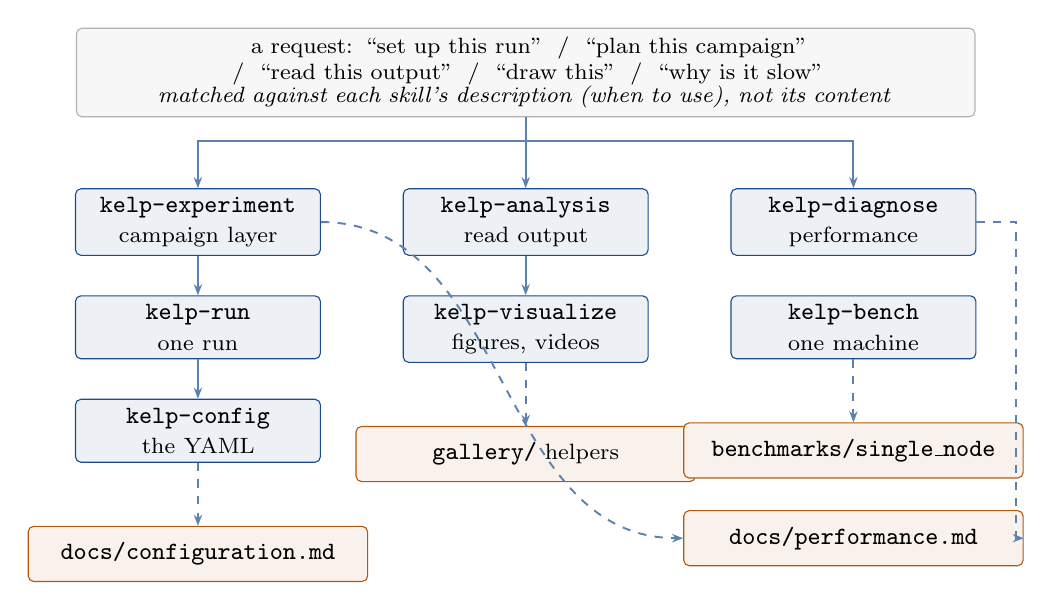
\begin{tikzpicture}[node distance=5mm and 7mm,
  sk/.style={rectangle,rounded corners=2pt,draw=lagblue,fill=lagblue!8,align=center,
             inner sep=3pt,minimum height=8mm,text width=29mm,font=\small},
  doc/.style={rectangle,rounded corners=2pt,draw=lagelem,fill=lagelem!8,align=center,
             inner sep=3pt,minimum height=7mm,text width=41mm,font=\footnotesize},
  req/.style={rectangle,rounded corners=2pt,draw=gray!60,fill=gray!6,align=center,
             inner sep=3pt,text width=112mm,font=\footnotesize},
  lk/.style={-{Stealth[length=4pt]},line width=0.7pt,draw=lagblue!70}]
  \node[req] (req) {a request: ``set up this run'' \;/\; ``plan this campaign'' \;/\; ``read this output''
    \;/\; ``draw this'' \;/\; ``why is it slow''\\[-1pt]
    \textit{matched against each skill's description (when to use), not its content}};
  \node[sk, below left=9mm and 26mm of req.south] (exp) {\code{kelp-experiment}\\\footnotesize campaign layer};
  \node[sk, below=of exp] (run) {\code{kelp-run}\\\footnotesize one run};
  \node[sk, below=of run] (cfg) {\code{kelp-config}\\\footnotesize the YAML};
  \node[sk, below=9mm of req.south] (ana) {\code{kelp-analysis}\\\footnotesize read output};
  \node[sk, below=of ana] (viz) {\code{kelp-visualize}\\\footnotesize figures, videos};
  \node[sk, below right=9mm and 26mm of req.south] (dia) {\code{kelp-diagnose}\\\footnotesize performance};
  \node[sk, below=of dia] (ben) {\code{kelp-bench}\\\footnotesize one machine};
  \node[doc, below=8mm of cfg] (d1) {\srcfile{docs/configuration.md}};
  \node[doc, below=8mm of viz] (d2) {\srcfile{gallery/} helpers};
  \node[doc, below=8mm of ben] (d4) {\srcfile{benchmarks/single\_node}};
  \node[doc, below=4mm of d4] (d3) {\srcfile{docs/performance.md}};
  \draw[lk] (req.south) -- ++(0,-3mm) -| (exp.north);
  \draw[lk] (req.south) -- (ana.north);
  \draw[lk] (req.south) -- ++(0,-3mm) -| (dia.north);
  \draw[lk] (exp) -- (run);  \draw[lk] (run) -- (cfg);
  \draw[lk] (ana) -- (viz);
  \draw[lk,dashed] (cfg) -- (d1); \draw[lk,dashed] (viz) -- (d2); \draw[lk,dashed] (ben) -- (d4);
  \draw[lk,dashed] (dia.east) -- ++(5mm,0) |- (d3.east);
  \draw[lk,dashed] (exp.east) to[out=0,in=180] (d3.west);
\end{tikzpicture}
\caption{How requests reach the skills. A request is matched against the skills' descriptions; the
selected \srcfile{SKILL.md} then points to the neighbouring skill it builds on (solid) and to the
documentation it defers to (dashed). Reference files under each skill's \srcfile{references/} are
opened only from the step that names them.}
\label{fig:skills-routing}
\end{figure}

\section{How the skill text is written}\label{sec:skills-design}

The skills are read by agents of different strength, and the way a rule is phrased decides whether
it is followed. The text therefore follows a small set of conventions.

\paragraph{Defaults and checks.} Each skill that produces a product opens with a short paragraph
that separates two kinds of guidance. \emph{Defaults} are the choices that worked in past work ---
a palette, a background, a layout, which tables to write, how an event is counted, which
uncertainty to quote. They are written as ``by default \dots; if the owner asks for something else,
do that'', because a default stated as a mandate makes a careful agent refuse what the owner
explicitly asked for. \emph{Checks} protect correctness whatever the style: the colour map's ends
agree with the label (an assertion in the script), dead particles are masked by status, lead times
are measured from each particle's own release, every number carries its denominator, cohorts the run
does not cover are dropped or censored, and a claim about a whole run is guarded by an assertion that
its last record is the run's end. Each check states its scope in the same sentence, so that
relaxing a default cannot silently relax the check. A handback ends with a section that lists every
default not used (with the owner's choice) and every check skipped (with the condition that did not
hold).

\paragraph{The launch gate.}\label{sec:skills-gate} The skills that prepare a run or a batch job (\code{kelp-run}, \code{kelp-config},
\code{kelp-experiment}) stop before starting it; the benchmark skill asks before running on a cluster
node. The prepared command is shown, and the agent asks for an explicit
confirmation of that command; a request that merely describes the run (``run it on 128 cores'') is
not a confirmation. The last line of their handback states that nothing was run.

\paragraph{Checks keyed to their condition.} A pre-launch check applies where its stated condition
holds: the vertical-velocity sign check for a three-dimensional run on a velocity not used before,
the record-0 check for a dataset not used before, the grid-hash cell check for a release in a
refined region of a non-uniform mesh. A check whose condition does not hold is skipped, with one
line saying why; the launch gate holds for every run.

\paragraph{Runnable code, no example numbers as answers.} Code blocks in the skills are complete
enough to run and were run before they were written down. Measured constants --- memory per particle and
throughput --- live in \srcfile{docs/performance.md} (a few per-event costs and the output sizing rule in
the skills' reference files, labelled as single measurements); a skill states the recipe that
derives the number for the task at hand and labels any quoted value as the measurement it came from.
A number from a worked example is never a substitute for the reader's own measurement.

\paragraph{Short entry files, reference files on demand.} Each \srcfile{SKILL.md} holds the routing,
the ordered workflow, the decision predicates and the checks; long templates and recipes live in
\srcfile{references/}. Two rules keep the split safe: the call line of every helper stays in the entry
file (a reader that never opens the reference still calls the helper correctly), and a reference that
depends on another links to it.

\section{The check scripts}\label{sec:skills-scripts}

Two pre-launch checks recur for every new dataset and are shipped as scripts, run from the clone
with the absolute path of the configuration.

\paragraph{Vertical-velocity sign.} \srcfile{w\_sign.py} loads the mesh and the dataset through the
configured reader with \conf{mode.w\_positive} forced to \code{up}, so that the negated internal
velocity is the file's own value (\cref{sec:vert-wsign}); it averages the file's vertical velocity
from \ang{2}\,S to \ang{2}\,N and from \ang{150}\,W to \ang{100}\,W, at the level nearest \SI{50}{m}, over records 1--30, and prints the mean with the sign
it implies. Equatorial upwelling makes the sign unambiguous there: a positive mean means the file
stores upward velocity. A store that does not cover this box stops with a request for another region
of known up- or downwelling. The configuration keeps \conf{w\_positive: auto} until the printed value
is written in, and the run script refuses \code{auto} for such a run.

\paragraph{Record 0.} \srcfile{record0.py} prints the fraction of exactly zero surface elevation at
the first, middle and last record. A model archive whose first record is the initial state of a cold
start shows a fraction near one there; the run then starts after the spin-up, which a periodic
forcing signal needs hours of records to develop --- skipping one record is not a spin-up.

\codeanchor{\srcfile{.claude/skills/kelp-run/scripts/w\_sign.py} and \srcfile{record0.py}; both use
\fn{load\_config}, \fn{get\_reader} and the reader's \fn{load\_mesh}, \fn{open\_dataset} and
\fn{read\_velocities}; \code{w\_sign.py} also uses \fn{unrotate\_lonlat} for a rotated mesh.}

\section{Skills and the documentation}\label{sec:skills-docs}

The skills are procedure; the documentation is reference. Option semantics, defaults and validation
rules are authoritative in \srcfile{docs/configuration.md}; the pipeline in
\srcfile{docs/architecture.md}; costs and sizing in \srcfile{docs/performance.md}; the restart
mechanics in \srcfile{docs/io\_and\_time.md}. A skill cites these rather than restating them, so that
a change in the engine is documented once. Where a skill and the documentation disagree, the
documentation and --- behind it --- the source take precedence, as throughout this manual.

\section{Maintaining a skill}\label{sec:skills-maintain}

A skill changes when a campaign shows that a step was missing, a rule was wrong, or a phrase led a
reader astray. Four practices keep the text reliable. Every code block in an edited skill is run
before it is committed. A changed rule is exercised by having a separate agent carry out a
representative task with the edited skill, and the artefact it produces --- not its summary --- is
reviewed, including a task in which the owner departs from a default on purpose, so that a new rule
does not override the owner. The review of an edit lists the errors the edit itself introduced, which
is where most new defects come from. Finally, the skills ship with the public engine: they carry
engineering practice and generic rules, and no study results.


\appendix
\chapter{Configuration Key Reference}\label{app:config}

This appendix lists the configuration keys consumed by the engine, grouped by their YAML
section. It is a reference companion to the chapters: each key is described in context in
the relevant chapter, and here we collect them with their types and defaults. The keys and
defaults follow the engine's configuration module.

\paragraph{Load rules.} A configuration must contain all five top-level sections
(\conf{mode}, \conf{numerics}, \conf{mesh}, \conf{data}, \conf{time}); a section that is
present but empty must be written as \code{\{\}}. Keys that are misspelled or of the wrong
case are silently ignored and the default is used --- there is no typographic protection ---
so a key that appears to have no effect should be checked against this table. Relative paths of the mesh,
data, seed and output files are resolved against the directory of the configuration file;
\conf{numerics.shared\_fields\_dir} is taken as written. Many values are validated when the file is
loaded --- the integrator, the interpolation methods \conf{uv\_interp}, \conf{w\_interp} and
\conf{sample\_interp}, the diffusion, beaching (when enabled), periodic, adaptive-scheme, grid-hash, rotation
and HEALPix keys, \conf{w\_positive}, \conf{uv\_vertical}, \conf{input\_rotation} and the stamp keys of
\conf{data} --- and an invalid value there raises an error immediately; others, such as
\conf{max\_levels}, \conf{time\_averaging} and the \conf{time} values, are checked when the run starts or
when first used. Unknown keys inside the diffusion and
beaching blocks are ignored like any other.

\setlength{\tabcolsep}{4pt}

\section*{\texttt{mode} --- tracking mode and variable names}
\begin{longtable}{@{}>{\ttfamily\footnotesize}p{0.295\linewidth} >{\footnotesize}p{0.075\linewidth} >{\footnotesize}p{0.095\linewidth} >{\footnotesize}p{0.37\linewidth}@{}}
\toprule
\normalfont Key & Type & Default & Description \\
\midrule \endhead
Fdrift2D & bool & \code{true} & Kept for older configurations; not read by the engine. \\
Fdrift3D & bool & \code{false} & Three-dimensional tracking with vertical velocity; alone decides between 2-D and 3-D. \\
time\_dir & float & \code{1.0} & Integration direction: \code{1.0} forward, \code{-1.0} backward; any other value is refused. \\
Vpuls & bool & \code{false} & FESOM-C 2-D only: add the pulsation velocity to the mean flow. \\
var\_u, var\_v & str & auto & Names of the horizontal velocity variables; set to \code{unod}/\code{vnod} for node-layout FESOM2 velocities (requires \conf{uv\_interp: barycentric}). \\
var\_w & str & auto & Name of the vertical velocity (3-D). FESOM2: if unresolved, the run proceeds in 2-D silently; FESOM-C refuses \code{w\_cart}. \\
w\_positive & str & \code{auto} & Sign convention of the vertical velocity in the file: \code{auto}, \code{up} or \code{down} (\cref{sec:vert-wsign}). \\
var\_eta & str & auto & Name of the sea-surface height. \\
uv\_vertical & str & \code{layer} & Horizontal velocity in depth: \code{layer} (constant within each layer) or \code{linear} (linear between the layer centres; a stencil member whose bed lies above the particle is a wall; \cref{sec:vert-uvdepth}). \code{linear} needs 3-D tracking (refused at load otherwise), a z-level or sigma mesh, \code{euler}, \code{rk2} or \code{rk4}, and \conf{uv\_interp} \code{barycentric} for node layout or \code{leastsq}, \code{edge\_leastsq} or \code{barycentric} for element layout; FESOM2 element data need the element bottoms and no ice-shelf cavities (\cref{sec:mesh-elem-bottoms}). Refused for \code{fesom14}, whose velocities on the levels are always linear in depth. Recorded as the output attribute \code{uv\_vertical = "linear"}; a resume must keep it (\cref{sec:out-restart}). \\
sigma\_layer & int & surface & 2-D layered input: which vertical layer to track (\code{fesom14}: a 0-based kept level). \\
sigma\_mean & bool & \code{false} & FESOM-C and \code{fesom14} 2-D: thickness-weighted vertical mean instead of one layer. \\
max\_levels & int & all & Keep the first $N$ vertical interfaces from the surface; must be $\ge 2$ in 3-D. \\
sample\_vars & list & \code{[]} & Node-based scalar fields to sample along trajectories (e.g.\ \code{temp}, \code{salt}). \\
track\_failure\_reason & bool & \code{false} & Record why each particle died (\cref{sec:life-reason}). \\
\bottomrule
\end{longtable}

\section*{\texttt{numerics} --- step, integrator, interpolation}
\begin{longtable}{@{}>{\ttfamily\footnotesize}p{0.295\linewidth} >{\footnotesize}p{0.075\linewidth} >{\footnotesize}p{0.095\linewidth} >{\footnotesize}p{0.37\linewidth}@{}}
\toprule
\normalfont Key & Type & Default & Description \\
\midrule \endhead
dt & float (s) & auto & Integration step. Defaults to the snapshot interval. In the discrete mode it must equal the record spacing, and irregular record times (calendar months) are refused --- use \conf{temporal\_interp}, where it may be smaller. \\
file\_dt & float (s) & auto & Time between stored snapshots; auto-detected from the time coordinate. When the axis cannot be decoded it defines $t_i=i\,\Delta t$ (\cref{sec:input-axis}). \\
integrator & str & \code{euler} & \code{euler} / \code{rk2} / \code{rk4} / \code{rk45} (\cref{ch:integration}). \\
rk45\_tol\_m & float (m) & \code{1.0} & Adaptive scheme: error tolerance per substep, $>0$ (\cref{sec:int-rk45}). \\
rk45\_h\_min & float (s) & $10^{-4}\dt$ & Adaptive scheme: smallest substep, $>0$. \\
output\_freq & int & \code{1} & Record positions every $N$ steps, counted from the start of the run. \\
temporal\_interp & bool & \code{false} & Reconstruct velocity in time between snapshots; permits sub-stepping (\cref{ch:temporal}). \\
temporal\_reconstruction & str & \code{linear} & \code{linear} or \code{pchip} (monotone cubic); active only with \conf{temporal\_interp}. \\
velocity\_float32 & bool & \code{false} & Hold velocity in single precision; halves snapshot memory. \\
prefetch\_size & int & \code{1} & Snapshots read per bulk read-ahead; forced to 1 under cyclic forcing and with the shared cache. \\
shared\_fields\_dir & str & \code{null} & Directory of the node-shared snapshot cache (\cref{sec:input-shared}). \\
shared\_fields\_generation & str & \code{null} & Namespace generation of the cache; else \code{KELP\_SHARED\_FIELDS\_GENERATION}, else the batch job. \\
checkpoint\_freq & int & \code{0} & Write a restart checkpoint every $N$ steps (\code{0} = off); needs an output path. \\
output\_flush\_every & int & \code{0} & NetCDF only: flush every $N$ records so the file is readable mid-run. \\
uv\_interp & str & \code{leastsq} & \code{leastsq} (element centres), \code{edge\_leastsq} (containing element and edge neighbours) or \code{barycentric} (vertex blend; required for node velocities) (\cref{ch:hvel}). \\
edge\_leastsq\_bc & str & \code{freeslip} & Wall ghost of \code{edge\_leastsq}: \code{freeslip} or \code{noslip}. \\
elem\_search & str & \code{local} & Containing element: \code{local} (search each step) or \code{walk} (track across edges; \cref{sec:loc-walk}). \\
w\_interp & str & \code{leastsq} & 3-D vertical-velocity horizontal combine: \code{nearest}/\code{leastsq}/\code{barycentric}/\code{idw}. \\
sample\_interp & str & \code{leastsq} & Horizontal method for sampled scalars (same options). \\
Dmin & float (m) & \code{0.5} & Minimum water-column thickness (sigma meshes only; \cref{sec:vert-clamp}). \\
z0b\_min & float (m) & \code{0.1} & Bottom clamp offset (sigma meshes only). \\
Dch & float & \code{1.0} & Reserved; currently unused. \\
periodic\_lon, periodic\_lat & [lo, hi] & \code{null} & Periodic windows for channel domains (\cref{sec:life-periodic}). \\
diffusion & map & off & Stochastic-diffusion sub-configuration (below). \\
beaching & map & off & Beaching sub-configuration (below). \\
\bottomrule
\end{longtable}

\section*{\texttt{numerics.diffusion}}
\begin{longtable}{@{}>{\ttfamily\footnotesize}p{0.295\linewidth} >{\footnotesize}p{0.075\linewidth} >{\footnotesize}p{0.095\linewidth} >{\footnotesize}p{0.37\linewidth}@{}}
\toprule
\normalfont Key & Type & Default & Description \\
\midrule \endhead
enabled & bool & \code{false} & Master switch; when off, byte-identical to no diffusion. \\
scheme & str & \code{uniform} & \code{uniform} / \code{em} (Euler--Maruyama) / \code{m1} (Milstein). Only \code{uniform} for the horizontal kick in 3-D. \\
kh\_zonal, kh\_meridional & float & \code{0.0} & Constant diffusivities (\code{uniform} only), m$^2$/s. \\
var\_kh\_zonal, var\_kh\_meridional & str & auto & Dataset diffusivity variable names (\code{em}/\code{m1}). \\
dres\_m & float (m) & auto & Central-difference offset for the diffusivity gradient. \\
seed & int & \code{0} & Counter-based RNG seed (\cref{sec:diff-rng}); restart-safe. \\
composition & str & \code{split} & How the kick composes with the step: \code{split}/\code{combined}/\code{split\_rk}. \\
kh\_eval\_position & str & \code{end} & \code{split\_rk} only: sample diffusivity at \code{start} or \code{end} of step. \\
az\_enabled & bool & \code{false} & Vertical random walk (\cref{sec:diff-vertical}); needs \conf{enabled} and the \code{uniform} scheme. \\
az\_const & float & \code{0.0} & Constant vertical diffusivity, m$^2$/s, $\ge 0$. \\
var\_az & str & \code{null} & Vertical diffusivity variable on the interfaces (FESOM2 z-level). \\
\bottomrule
\end{longtable}

\section*{\texttt{numerics.beaching}}
\begin{longtable}{@{}>{\ttfamily\footnotesize}p{0.295\linewidth} >{\footnotesize}p{0.075\linewidth} >{\footnotesize}p{0.095\linewidth} >{\footnotesize}p{0.37\linewidth}@{}}
\toprule
\normalfont Key & Type & Default & Description \\
\midrule \endhead
enabled & bool & \code{false} & Master switch (\cref{sec:life-beach}). \\
criteria & list & \code{[depth]} & Any of \code{depth}, \code{coastal\_element}, \code{on\_failure}, \code{stochastic}; combined inclusively. \\
depth\_min & float (m) & \code{0.3} & Strand when the column height falls below this. \\
use\_eta & bool & \code{false} & Include sea level in the column height (needs an ssh field). \\
dry\_mask\_var & str & none & Node variable marking dry cells ($>0.5$); strands (with the \code{depth} criterion) and blocks resuspension. \\
zone\_depth & float (m) & auto & Near-shore zone for stochastic stranding; defaults to twice \conf{depth\_min}. \\
t\_beach & float (s) & \code{86400} & Stochastic stranding timescale: $P=1-\exp(-|\dt|/t_{\text{beach}})$ per step. \\
resuspension & str & \code{never} & One of \code{never}, \code{auto}, \code{stochastic}, or \code{auto\_or\_stochastic}. \\
rewet\_hysteresis & float (m) & \code{0.1} & Margin above \conf{depth\_min} to count as re-wetted. \\
min\_wet\_steps & int & \code{1} & Consecutive wet steps before automatic release. \\
t\_resuspend & float (s) & none & Stochastic-release timescale (required for stochastic resuspension). \\
seed & int & none & Beaching RNG seed; defaults to the diffusion seed. \\
\bottomrule
\end{longtable}

\section*{\texttt{mesh} --- mesh source}
\begin{longtable}{@{}>{\ttfamily\footnotesize}p{0.295\linewidth} >{\footnotesize}p{0.075\linewidth} >{\footnotesize}p{0.095\linewidth} >{\footnotesize}p{0.37\linewidth}@{}}
\toprule
\normalfont Key & Type & Default & Description \\
\midrule \endhead
type & str & \code{fesomc} & \code{fesom2} / \code{fesom14} / \code{fesomc} / \code{nemo} / \code{healpix}; selects the reader, conventions, and vertical coordinate. \code{fesom14} needs \conf{uv\_interp: barycentric} (\cref{sec:mesh-fesom14}). \\
meshpath & str & required & Path to the mesh file or directory (\cref{ch:mesh}). \code{fesom14}: an ASCII mesh directory (it holds \code{nod3d.out}), or level-wise data with cell polygons --- a file, or a directory whose first \code{*.nc} file holding \conf{mode.var\_u} is used. \\
input\_rotation & [3 floats] & \code{null} & \code{fesom14} only (refused at load for every other type): the Euler angles in degrees, from the run's namelist, of the rotated frame an ASCII mesh is stored in; rotated back to geographic on load. Refused for a mesh from cell polygons; independent of \conf{rotation}. \\
r\_earth & float (m) & family & Earth radius for mesh-derived areas; defaults per model. \\
rotation & varies & \code{null} & FESOM2, FESOM~1.4 and HEALPix: \code{null} (geographic), \code{fesom2}, or an explicit list of Euler angles (\cref{ch:frame}). \\
exact\_nearest & bool & \code{true} & Prove every nearest-node anchor (\cref{sec:loc-exact}). \\
grid\_hash\_cell\_rule & str & \code{occu-} \code{pancy} & Choose the hash cell by measurement (\code{occupancy}), or keep the reader's (\code{legacy}) (\cref{sec:loc-cell}). \\
grid\_hash\_cell\_size & float (deg) & \code{null} & Explicit hash cell; overrides the rule. \\
healpix\_zoom & int & \code{null} & HEALPix: zoom level when the store carries no grid attributes. \\
healpix\_geometry & str & \code{dual} & HEALPix: \code{dual} (nodes at pixel centres) or \code{pixel} (elements are pixels; 2-D). \\
crop\_bbox & [W, E, S, N] & \code{null} & HEALPix: crop to a box; $W>E$ crosses the dateline. \\
levels & path or list & \code{null} & HEALPix: interface depths, a level-table path or an inline list; needed in 3-D, and in 2-D it sets the node depths when the store has no bathymetry variable. \\
\bottomrule
\end{longtable}

\section*{\texttt{data} --- input and output}
\begin{longtable}{@{}>{\ttfamily\footnotesize}p{0.295\linewidth} >{\footnotesize}p{0.075\linewidth} >{\footnotesize}p{0.095\linewidth} >{\footnotesize}p{0.37\linewidth}@{}}
\toprule
\normalfont Key & Type & Default & Description \\
\midrule \endhead
ncinput & str & required & Velocity input: a file, a Zarr store, or (FESOM2) a directory of per-variable files; \code{fesom14}: a file, a directory or a glob, the files grouped by the variables they hold (\cref{sec:input-reader}). \\
ncinput\_v & str & \code{""} & Separate $v$-velocity file, if not in \conf{ncinput} (NEMO: overrides grid-V; HEALPix: refused). \\
ncinput\_w & str & \code{""} & Separate vertical-velocity file (3-D), if applicable (HEALPix: refused). \\
ncinput\_eta & str & \code{""} & HEALPix: separate sea-surface-height store. \\
inicloud & str & required & Release positions: rows of \code{lon lat [depth] [release\_sec]}, geographic (\cref{sec:life-release}). \\
particle\_offset & int & \code{null} & Global index of the file's first particle in a sharded release (\cref{sec:perf-shard}); \code{null} = the file's \code{\# kelp particle\_offset N} header, else 0. Keys every random draw. \\
output\_path & str & memory & Output; \code{.zarr} selects Zarr, otherwise NetCDF4 (\cref{ch:output}). \\
time\_averaging & str & guess & \code{mean} (shift timestamps to window midpoints) or \code{instant}; set explicitly (guess: \code{mean} for FESOM2 and HEALPix). \code{fesom14}: leave unset --- the reader resolves the record times itself and a set value is refused; the output records \code{"resolved\_by\_reader"} (\cref{sec:input-timeavg}). \\
time\_stamp & str & \code{null} & \code{fesom14} only (the three stamp keys are refused for every other type): where a stamp sits in its window, \code{start}, \code{centre} or \code{end}, or \code{instant} for snapshots. Given together with \conf{time\_window} or not at all; overrides the files' time bounds or output schedule with a warning. \\
time\_window & str & \code{null} & \code{fesom14} only: the averaging window (with \code{instant}, the snapshot cadence): \code{calendar\_month}, \code{calendar\_year}, \code{calendar\_day} or a duration \code{"<number> <s|min|h|d>"}, computed in the files' calendar. \\
time\_offset & str & \code{null} & \code{fesom14} only: a shift \code{"<$\pm$number> <s|min|h|d>"} added to the stamps, bounds and epoch of every file first, for raw output of a job that started after midnight; allowed alone. \\
\bottomrule
\end{longtable}

\section*{\texttt{time} --- window and realizations}
\begin{longtable}{@{}>{\ttfamily\footnotesize}p{0.295\linewidth} >{\footnotesize}p{0.075\linewidth} >{\footnotesize}p{0.095\linewidth} >{\footnotesize}p{0.37\linewidth}@{}}
\toprule
\normalfont Key & Type & Default & Description \\
\midrule \endhead
start\_time\_idx & int & \code{0} & First snapshot index to read. \\
n\_steps & int & --- & Number of integration steps (preferred way to set the length). \\
end\_time\_idx & int & --- & Legacy alternative to \conf{n\_steps}. \\
start\_date & str & --- & Start as an ISO date in the axis calendar; between snapshots only with \conf{temporal\_interp} (\cref{sec:input-window}). \\
duration\_days & float & --- & With \conf{start\_date}: run length in days, $\lfloor\text{days}\cdot86400/\dt\rfloor$ steps. \\
on\_exhausted & str & \code{stop} & At the end of the forcing: \code{stop} or \code{cycle} (wrap). \\
num\_runs & int & \code{1} & Independent realizations (ensemble; \cref{ch:diffusion}). \\
run\_interval & int & \code{0} & Snapshot-index offset between successive realizations. \\
n\_pulses & int & \code{1} & Re-release the seed set this many times (\cref{sec:life-release}). \\
pulse\_interval & float (s) & \code{0.0} & Interval between pulses (required when \conf{n\_pulses} $>1$). \\
\bottomrule
\end{longtable}

\section*{Command line}
The command \code{kelp run config.yaml} runs a configuration, \code{kelp info config.yaml} prints the mesh and
the time range without tracking, and \code{kelp --version} prints the engine version. The options of \code{kelp run} override the corresponding keys:

\begin{longtable}{@{}>{\ttfamily\footnotesize}p{0.295\linewidth} >{\footnotesize}p{0.58\linewidth}@{}}
\toprule
\normalfont Option & Effect \\
\midrule \endhead
-o, --output & Output path; overrides \conf{data.output\_path}. \\
--checkpoint-freq N & Overrides \conf{numerics.checkpoint\_freq}. \\
--temporal-interp & Switches the interpolated mode on; without the option the configuration decides. \\
--seed N & Overrides \conf{numerics.diffusion.seed}. \\
--flush-every N & Overrides \conf{numerics.output\_flush\_every}. \\
-v, --verbose & Per-step timing with the phase split of \cref{sec:perf-measure}. \\
\bottomrule
\end{longtable}

\chapter{Notation and Symbols}\label{app:notation}

This appendix collects the principal symbols used in the manual. The sign and unit
conventions they obey are stated in the front-matter section ``Notation and conventions''.

\begin{longtable}{@{}l p{0.72\linewidth}@{}}
\toprule
Symbol & Meaning \\
\midrule \endhead
$\pos=(\lonx,\latx,\depx)$ & Particle position: longitude, latitude (degrees), depth (m, positive down). \\
$\velvec=(u,v,\Wvel)$ & Velocity: horizontal components (m\,s$^{-1}$) and vertical velocity $\Wvel$ (m\,s$^{-1}$, positive down). \\
$t,\ \dt$ & Time and the (positive) integration step. \\
$\tdir$ & Integration-direction factor, $+1$ forward or $-1$ backward (the key \conf{time\_dir}). \\
$\Mlat$ & Metres per degree of latitude, $\SI{111120}{\metre\per\degree}$. \\
$\zzero$ & Metres per degree of longitude, $\max(\cos\latx\,\Mlat,1)$. \\
$\bwt{i}$ & Barycentric / Wachspress interpolation weight at vertex $i$. \\
$\interpfrac$ & Interpolation fraction, in time (\cref{eq:temp-linear}) or in depth (\cref{eq:vert-alpha}). \\
$N,\ E,\ K$ & Number of mesh nodes, elements, and vertical interfaces ($K-1$ layers). \\
$z_k$ & Depth of the $k$-th vertical interface. \\
$\sigma_k$ & Sigma value of the $k$-th interface (FESOM-C); $\sigma=1$ surface, $\sigma=0$ floor. \\
$H$ & Sigma-mesh water-column thickness, $\max(d+\eta,D_{\min})$. \\
$d,\ \eta$ & Still-water depth and sea-surface height. \\
$D_{\min},\ z_{0b}$ & Minimum column thickness and bottom clamp offset (sigma; keys \conf{Dmin}, \conf{z0b\_min}). \\
$K_h$ & Horizontal eddy diffusivity (m$^2$\,s$^{-1}$); $\sigma^2=2K_h t$. \\
$R$ & Earth radius of the mesh (\conf{mesh.r\_earth}), used in the local tangent-plane projection. \\
$R_M$ & Metric radius of the displacement, $\Mlat\cdot180/\pi$, used by the great-circle kicks (\cref{sec:diff-sphere}). \\
$\xi,\ \xi_1,\ \xi_2$ & Standard normal variates of the stochastic kicks (\cref{ch:diffusion}). \\
$A_z$ & Vertical eddy diffusivity (m$^2$\,s$^{-1}$), \cref{sec:diff-vertical}. \\
$c_k$ & Fraction of the step at which Runge--Kutta stage $k$ samples the flow. \\
$p_k,\ M$ & Data points of a depth-linear horizontal velocity (layer centres or levels; on a sigma mesh layer centres in $s$) and their number (\cref{sec:vert-uvdepth}). \\
$\ell_c,\ d_c,\ D_c$ & Last usable data point, bed depth and reader-declared data prefix of column $c$ (a node or an element), \cref{eq:vert-uv-last}. \\
$s$ & Sigma fraction $z/H_p$ of the particle's column, clipped to $[0,1]$ (\cref{eq:vert-uv-sigma}). \\
$\bwt{i}^{+}$ & Barycentric weight counted as zero when negative, in the wall rule (\cref{eq:vert-uv-bary}). \\
$\alpha_0,\ \alpha_k$ & Bracket fraction of a lazy blend and stage fraction of a stage blend (\cref{ch:temporal}). \\
$A_k,\ C_k$ & Doubled fan- and corner-triangle areas in the Wachspress weights (\cref{eq:wachspress}). \\
\bottomrule
\end{longtable}

\chapter{Source-Code Map}\label{app:codemap}

This appendix maps each subsystem of the engine to the source files that implement it and to the chapter that
describes it, so that a reader starting from the code can find the corresponding text and vice versa. Paths are
relative to the package source root, \code{src/kelp/}, unless they begin with the repository directory
\code{utils/} or \code{.claude/}.

\begin{longtable}{@{}>{\footnotesize}p{0.34\linewidth} >{\ttfamily\footnotesize\raggedright\arraybackslash}p{0.40\linewidth} >{\footnotesize}l@{}}
\toprule
\normalfont Subsystem & \normalfont Principal source & \normalfont Manual \\
\midrule \endhead
Run orchestration & tracking.py & \cref{ch:arch} \\
Command line & cli/main.py & \cref{app:config} \\
Mesh structure, contract \& derived tables & core/mesh.py & \cref{ch:mesh} \\
FESOM2 and FESOM-C meshes & readers/fesom2.py, readers/fesomc.py & \cref{ch:mesh} \\
HEALPix meshes and reader & readers/healpix.py & \cref{ch:mesh,ch:input} \\
Structured grids and NEMO & readers/structured.py, readers/nemo.py & \cref{ch:mesh,ch:input} \\
Nearest node: grid hash, cell rule, exact search & core/mesh.py, utils/check\_grid\_hash\_cell.py & \cref{ch:localization} \\
Containment and element tracking & core/mesh.py, numerics/integrators.py & \cref{sec:loc-contain,sec:loc-walk} \\
Horizontal velocity interpolation & numerics/interpolate.py & \cref{ch:hvel} \\
Polygon weights (triangle / Wachspress) & core/mesh.py & \cref{sec:hvel-quad} \\
Vertical geometry \& $\Wvel$ (z-level) & numerics/vertical.py & \cref{ch:vertical} \\
Vertical geometry \& $\Wvel$ (sigma) & numerics/vertical\_sigma.py & \cref{ch:vertical} \\
Vertical-velocity sign & readers/\_\_init\_\_.py & \cref{sec:vert-wsign} \\
Offline vertical-velocity reconstruction & w\_reconstruct.py, utils/reconstruct\_w.py & \cref{sec:vert-wsign} \\
Scalar sampling & numerics/sampling.py & \cref{ch:sampling} \\
Coordinate frame / rotation & core/rotation.py, readers/fesom2.py, readers/healpix.py, tracking.py & \cref{ch:frame} \\
Time integration & numerics/integrators.py & \cref{ch:integration} \\
Fused kernels & numerics/integrators.py, numerics/interpolate.py & \cref{ch:fused} \\
Temporal reconstruction & numerics/temporal\_reconstruct.py, core/io.py & \cref{ch:temporal} \\
Stochastic diffusion & numerics/diffusion.py & \cref{ch:diffusion} \\
Particle state \& lifecycle & core/particles.py, core/release.py & \cref{ch:lifecycle} \\
Seeding helpers & core/particles\_gen.py & \cref{ch:lifecycle} \\
Beaching & numerics/beaching.py, tracking.py & \cref{sec:life-beach} \\
Periodic windows & tracking.py & \cref{sec:life-periodic} \\
Forcing readers \& time axis & readers/, tracking.py & \cref{ch:input} \\
Step payload \& snapshot cache & core/io.py, tracking.py & \cref{sec:input-payload} \\
Node-shared snapshot cache & core/shared\_fields.py & \cref{sec:input-shared} \\
Trajectory output \& restart & writers.py & \cref{ch:output} \\
Sharding and merging & utils/sort\_seeds.py, utils/split\_seeds.py, utils/concat\_trajectories.py & \cref{sec:out-merge,sec:perf-shard} \\
Plotting and statistics & visualization/ (plots, animation, presence statistics) & --- (module README) \\
Region extraction & utils/extract\_fesom\_region.py, utils/extract\_healpix\_region.py & \cref{sec:perf-io} \\
Configuration & core/config.py & \cref{app:config} \\
Spherical metric / constants & core/geometry.py & \cref{sec:int-metric} \\
Agent skills & .claude/skills/ & \cref{ch:skills} \\
\bottomrule
\end{longtable}

\noindent The package installs with \code{pip install -e .} from the repository root and provides the
\code{kelp} command. Every output records the engine version --- the package version and the commit ---
in its attributes, so a result can be traced to the source that produced it. The documentation tree carries a
machine-readable map from each subsystem to the source symbols and the revision at which its documentation was
last verified (\code{docs/doc\_map.yaml}), and a script that reports which documents have fallen behind their
code (\code{docs/check\_doc\_sync.py}).

\chapter{Glossary}\label{app:glossary}

\begin{description}[style=nextline,leftmargin=0pt,font=\normalfont\bfseries]
\item[FESOM family] The unstructured-mesh ocean models the engine principally targets:
  FESOM2 and FESOM-C. Used here as a collective term; statements specific to one model name it.
\item[FESOM2] A global ocean model on a purely triangular mesh with a fixed depth-level
  (z-level) vertical coordinate. The running example uses a FESOM2 mesh.
\item[FESOM-C] A coastal ocean model on a mixed mesh --- elements may be triangles or
  quadrilaterals --- with a terrain-following (sigma) vertical coordinate.
\item[Node] A vertex of the mesh. Node-layout fields (e.g.\ \code{unod}/\code{vnod},
  scalars, sea-surface height) are defined at nodes.
\item[Element] A mesh face: a triangle (FESOM2) or a triangle or quadrilateral (FESOM-C, HEALPix,
  NEMO). Element-layout velocities are defined at element centroids.
\item[Interface, layer] The vertical level boundaries (interfaces) and the volumes between
  them (layers); $K$ interfaces bound $K-1$ layers. The vertical velocity lives at
  interfaces, the three-dimensional horizontal velocity and scalars at mid-layers.
\item[One-ring] The set of elements that share a given node; the stencil used by the
  localization search and several interpolators.
\item[Barycentric coordinates] The area-ratio weights of a point within a triangle, used to
  blend the three vertex values; the triangular interpolation stencil.
\item[Wachspress coordinates] The generalization of barycentric coordinates to a convex
  polygon, used to interpolate over a quadrilateral element; computed in a division-free product form
  that is exact on edges, which is why quadrilaterals must be convex.
\item[z-level coordinate] A vertical coordinate with fixed interface depths, the same
  everywhere (FESOM2).
\item[Sigma coordinate] A terrain-following vertical coordinate whose interface depths are
  fractions of the local column thickness $H=\max(d+\eta,D_{\min})$ (FESOM-C).
\item[Node-layout / element-layout] Whether a velocity field is stored at nodes or at
  element centroids; node layout admits only the barycentric scheme, element layout all three.
\item[Fused / unfused kernel] The two interchangeable implementations of a step: a single
  compiled loop over the particles, or separate parallel passes; they agree bit-for-bit where both exist.
\item[PCHIP] Monotone piecewise-cubic Hermite reconstruction of the velocity in time, using
  four snapshots; raises the realized temporal order above the linear reconstruction's cap.
\item[Counter-based RNG] A stateless random-number generator in which each draw is a hash of
  an integer key, giving results independent of thread count and reproducible across restarts.
\item[Beaching] The optional stranding of particles in shallow or coastal water, with an
  optional resuspension; the only reversible non-alive status.
\item[\code{time\_dir}] The integration-direction factor ($+1$ forward, $-1$ backward),
  folded into the interpolated velocity so the step size stays positive.
\item[Drifter / particle] A passive Lagrangian tracer advected by the flow; ``drifter'' is
  used in the schematics for the point being interpolated to.
\item[HEALPix] A hierarchical equal-area grid of the sphere on which some ocean products are stored; the
  engine builds a mesh from its pixel centres (dual mesh) or from its pixels (pixel mesh).
\item[Grid hash] The uniform lattice of cells over which mesh nodes are bucketed for the nearest-node
  search; its cell is chosen by measurement for each run.
\item[Exact anchor] A nearest node proven to be the nearest by the cap certificate of the search, the
  default since September 2026.
\item[Edge walk] Tracking the containing element from step to step by crossing element edges, instead of
  searching around the nearest node every time.
\item[Edge least squares] The velocity interpolation that fits a plane to the containing element and its
  edge neighbours, with mirrored ghost values at the coast.
\item[Adjoint process] The backward-in-time counterpart of an advection--diffusion process: the advection
  reversed, the diffusive drift and noise unchanged.
\item[Resumable chain] A long run split into consecutive batch jobs, each resuming from the previous one's
  restart; the concatenated result equals one uninterrupted run.
\item[Shard] One contiguous block of a large release, run as a separate process and merged back afterwards.
\item[Agent skill] A packaged set of instructions, reference files and check scripts that a coding agent
  loads to carry out one kind of task on the engine (\cref{ch:skills}).
\end{description}


\backmatter
\bibliographystyle{plainnat}
\bibliography{refs}
\printindex
\end{document}
